%%==================================================
%% diss.tex for SJTU Bachelor Thesis
%% based on CASthesis
%% version: 0.3a
%% Encoding: UTF-8
%%==================================================

% 字号选项: c5size 五号(默认) cs4size 小四
% 双面打印(注意字号设置)
%\documentclass[cs4size, a4paper, twoside]{sjtuthesis} 
% 单面打印(注意字号设置)
\documentclass[cs4size, a4paer, oneside, openany]{sjtuthesis} 


% \usepackage[sectionbib]{chapterbib}%每章都用参考文献
\usepackage{setspace}
\newboolean{DOIT}
\setboolean{DOIT}{false}%编译某些只想自己看的内容,编译true,否则false

%% 行距缩放因子(x倍字号)
\renewcommand{\baselinestretch}{1.3}

% 设置图形文件的搜索路径
\graphicspath{{figure/}{figures/}{logo/}{logos/}{graph/}{graphs}}

%%========================================
%% 在sjtuthesis.cls中定义的有用命令
%%========================================
% \cndash 中文破折号
% 数学常量
% \me 对数常数e
% \mi 虚数单位i
% \mj 虚数单位j
% \dif 直立的微分算符d为直立体。
% 可伸长的数学箭头、等号
% \myRightarrow{}{}
% \myLeftarrow{}{}
% \myBioarrow{}{}
% \myLongEqual{}{}
% 参考文献
% \upcite{} 上标引用
%%========================================


\begin{document}

%%%%%%%%%%%%%%%%%%%%%%%%%%%%%% 
%% 封面
%%%%%%%%%%%%%%%%%%%%%%%%%%%%%% 

% 中文封面内容(关注内容而不是形式)
\title{多功能模块化移动机器人的控制系统设计}
\author{崔运凯}
\advisor{费燕琼教授}
\degree{学士}
\defenddate{2010年6月4日}
\school{上海交通大学}
\institute{机械与动力工程学院}
\studentnumber{5090209365}
\major{机械电子}

% 英文封面内容(关注内容而不是表现形式)
\englishtitle{Design of a Multifunctional Mobile Modular Robot System}
\englishauthor{\textsc{Yunkai Cui}}
\englishadvisor{Prof. \textsc{Feiyan Qiong}}
\englishschool{Shanghai Jiao Tong University}
\englishinstitute{\textsc{Department of Mechanical Engineering and Automation, School of Mechanical Engineering} \\
  \textsc{Shanghai Jiao Tong University} \\
  \textsc{Shanghai, P.R.China}}
\englishdegree{Bachelor}
\englishmajor{Mechanical Engineering}
\englishdate{Jun. 4th, 2010}

% 封面
\maketitle

% 英文封面
\makeenglishtitle

% 论文原创性声明和使用授权
\makeDeclareOriginal
\makeDeclareAuthorization

%%%%%%%%%%%%%%%%%%%%%%%%%%%%%% 
%% 前言
%%%%%%%%%%%%%%%%%%%%%%%%%%%%%% 
\frontmatter

% 摘要
%%==================================================
%% abstract.tex for SJTU Bachelor Thesis
%% version: 0.5.2
%% Encoding: UTF-8
%%==================================================

\begin{abstract}

  上海交通大学是我国历史最悠久的高等学府之一,是教育部直属、教育部与上海市共建的全国重点大学,是国家 “七五”、“八五”重点建设和“211工程”、“985工程”的首批建设高校。经过115年的不懈努力,上海交通大学已经成为一所“综合性、研究型、国际化”的国内一流、国际知名大学,并正在向世界一流大学稳步迈进。 

 十九世纪末,甲午战败,民族危难。中国近代著名实业家、教育家盛宣怀和一批有识之士秉持“自强首在储才,储才必先兴学”的信念,于1896年在上海创办了交通大学的前身——南洋公学。建校伊始,学校即坚持“求实学,务实业”的宗旨,以培养“第一等人才”为教育目标,精勤进取,笃行不倦,在二十世纪二三十年代已成为国内著名的高等学府,被誉为“东方MIT”。抗战时期,广大师生历尽艰难,移转租界,内迁重庆,坚持办学,不少学生投笔从戎,浴血沙场。解放前夕,广大师生积极投身民主革命,学校被誉为“民主堡垒”。

 新中国成立初期,为配合国家经济建设的需要,学校调整出相当一部分优势专业、师资设备,支持国内兄弟院校的发展。五十年代中期,学校又响应国家建设大西北的号召,根据国务院决定,部分迁往西安,分为交通大学上海部分和西安部分。1959年3月两部分同时被列为全国重点大学,7月经国务院批准分别独立建制,交通大学上海部分启用“上海交通大学”校名。历经西迁、两地办学、独立办学等变迁,为构建新中国的高等教育体系,促进社会主义建设做出了重要贡献。六七十年代,学校先后归属国防科工委和六机部领导,积极投身国防人才培养和国防科研,为“两弹一星”和国防现代化做出了巨大贡献。

   改革开放以来,学校以“敢为天下先”的精神,大胆推进改革:率先组成教授代表团访问美国,率先实行校内管理体制改革,率先接受海外友人巨资捐赠等,有力地推动了学校的教学科研改革。1984年,邓小平同志亲切接见了学校领导和师生代表,对学校的各项改革给予了充分肯定。在国家和上海市的大力支持下,学校以“上水平、创一流”为目标,以学科建设为龙头,先后恢复和兴建了理科、管理学科、生命学科、法学和人文学科等。1999年,上海农学院并入;2005年,与上海第二医科大学强强合并。至此,学校完成了综合性大学的学科布局。近年来,通过国家“985工程”和“211工程”的建设,学校高层次人才日渐汇聚,科研实力快速提升,实现了向研究型大学的转变。与此同时,学校通过与美国密西根大学等世界一流大学的合作办学,实施国际化战略取得重要突破。1985年开始闵行校区建设,历经20多年,已基本建设成设施完善,环境优美的现代化大学校园,并已完成了办学重心向闵行校区的转移。学校现有徐汇、闵行、法华、七宝和重庆南路(卢湾)5个校区,总占地面积4840亩。通过一系列的改革和建设,学校的各项办学指标大幅度上升,实现了跨越式发展,整体实力显著增强,为建设世界一流大学奠定了坚实的基础。

  交通大学始终把人才培养作为办学的根本任务。一百多年来,学校为国家和社会培养了20余万各类优秀人才,包括一批杰出的政治家、科学家、社会活动家、实业家、工程技术专家和医学专家,如江泽民、陆定一、丁关根、汪道涵、钱学森、吴文俊、徐光宪、张光斗、黄炎培、邵力子、李叔同、蔡锷、邹韬奋、陈敏章、王振义、陈竺等。在中国科学院、中国工程院院士中,有200余位交大校友;在国家23位“两弹一星”功臣中,有6位交大校友;在18位国家最高科学技术奖获得者中,有3位来自交大。交大创造了中国近现代发展史上的诸多“第一”:中国最早的内燃机、最早的电机、最早的中文打字机等;新中国第一艘万吨轮、第一艘核潜艇、第一艘气垫船、第一艘水翼艇、自主设计的第一代战斗机、第一枚运载火箭、第一颗人造卫星、第一例心脏二尖瓣分离术、第一例成功移植同种原位肝手术、第一例成功抢救大面积烧伤病人手术等,都凝聚着交大师生和校友的心血智慧。改革开放以来,一批年轻的校友已在世界各地、各行各业崭露头角。

 截至2011年12月31日,学校共有24个学院/直属系(另有继续教育学院、技术学院和国际教育学院),19个直属单位,12家附属医院,全日制本科生16802人、研究生24495人(其中博士研究生5059人);有专任教师2979名,其中教授835名;中国科学院院士15名,中国工程院院士20名,中组部“千人计划”49名,“长江学者”95名,国家杰出青年基金获得者80名,国家重点基础研究发展计划(973计划)首席科学家24名,国家重大科学研究计划首席科学家9名,国家基金委创新研究群体6个,教育部创新团队17个。

  学校现有本科专业68个,涵盖经济学、法学、文学、理学、工学、农学、医学、管理学和艺术等九个学科门类;拥有国家级教学及人才培养基地7个,国家级校外实践教育基地5个,国家级实验教学示范中心5个,上海市实验教学示范中心4个;有国家级教学团队8个,上海市教学团队15个;有国家级教学名师7人,上海市教学名师35人;有国家级精品课程46门,上海市精品课程117门;有国家级双语示范课程7门;2001、2005和2009年,作为第一完成单位,共获得国家级教学成果37项、上海市教学成果157项。

  \keywords{上海交大,饮水思源,爱国荣校}
\end{abstract}

\begin{englishabstract}

An imperial edict issued in 1896 by Emperor Guangxu, established Nanyang Public School in Shanghai. The normal school, school of foreign studies, middle school and a high school were established. Sheng Xuanhuai, the person responsible for proposing the idea to the emperor, became the first president and is regarded as the founder of the university.

During the 1930s, the university gained a reputation of nurturing top engineers. After the foundation of People's Republic, some faculties were transferred to other universities. A significant amount of its faculty were sent in 1956, by the national government, to Xi'an to help build up Xi'an Jiao Tong University in western China. Afterwards, the school was officially renamed Shanghai Jiao Tong University.

Since the reform and opening up policy in China, SJTU has taken the lead in management reform of institutions for higher education, regaining its vigor and vitality with an unprecedented momentum of growth. SJTU includes five beautiful campuses, Xuhui, Minhang, Luwan Qibao, and Fahua, taking up an area of about 3,225,833 m2. A number of disciplines have been advancing towards the top echelon internationally, and a batch of burgeoning branches of learning have taken an important position domestically.

Today SJTU has 31 schools (departments), 63 undergraduate programs, 250 masters-degree programs, 203 Ph.D. programs, 28 post-doctorate programs, and 11 state key laboratories and national engineering research centers.

SJTU boasts a large number of famous scientists and professors, including 35 academics of the Academy of Sciences and Academy of Engineering, 95 accredited professors and chair professors of the "Cheung Kong Scholars Program" and more than 2,000 professors and associate professors.

Its total enrollment of students amounts to 35,929, of which 1,564 are international students. There are 16,802 undergraduates, and 17,563 masters and Ph.D. candidates. After more than a century of operation, Jiao Tong University has inherited the old tradition of "high starting points, solid foundation, strict requirements and extensive practice." Students from SJTU have won top prizes in various competitions, including ACM International Collegiate Programming Contest, International Mathematical Contest in Modeling and Electronics Design Contests. Famous alumni include Jiang Zemin, Lu Dingyi, Ding Guangen, Wang Daohan, Qian Xuesen, Wu Wenjun, Zou Taofen, Mao Yisheng, Cai Er, Huang Yanpei, Shao Lizi, Wang An and many more. More than 200 of the academics of the Chinese Academy of Sciences and Chinese Academy of Engineering are alumni of Jiao Tong University.

  \englishkeywords{\large SJTU, master thesis, XeTeX/LaTeX template}
\end{englishabstract}


% 目录
\tableofcontents
% 表格索引
\listoftables
% 插图索引
\listoffigures

% \addcontentsline{toc}{chapter}{\listfigurename} %将表格索引加入全文目录
% \addcontentsline{toc}{chapter}{\listtablename}  %将图索引加入全文目录

% 主要符号、缩略词对照表
% %%==================================================
%% symbol.tex for SJTU Bachelor Thesis
%% version: 0.5.2
%% Encoding: UTF-8
%%==================================================

\chapter{主要符号对照表}
\label{chap:symb}
\begin{tabular}{ll}

 \hspace{2em}$\epsilon$       & \hspace{5em}介电常数 \\
 \hspace{2em}$\mu$ \qquad     & \hspace{5em}磁导率 \\
  \hspace{2em}$\epsilon$       & \hspace{5em}介电常数 \\
 \hspace{2em}$\mu$ \qquad     & \hspace{5em}磁导率 \\
 \hspace{2em}$\epsilon$       & \hspace{5em}介电常数 \\
 \hspace{2em}$\mu$ \qquad     & \hspace{5em}磁导率 \\
 \hspace{2em}$\epsilon$       & \hspace{5em}介电常数 \\
 \hspace{2em}$\mu$ \qquad     & \hspace{5em}磁导率 \\


\end{tabular}


%%%%%%%%%%%%%%%%%%%%%%%%%%%%%% 
%% 正文
%%%%%%%%%%%%%%%%%%%%%%%%%%%%%% 
\mainmatter


%% 各章正文内容
%%==========================
%% chapter1.tex for SJTU Bachelor Thesis
%% content: introduction
%% version: 0.0.1
%% Encoding: UTF-8
%%==================================================

%\bibliographystyle{sjtu2} %[此处用于每章都生产参考文献]
\chapter{绪论}
\label{chap:introduction}

\section{模块化机器人的研究背景}

随着控制理论,传感器,计算机科学和人工智能等技术的发展,机器人的研究越来越受到关注。从上世纪90年代至今,机器人技术得到了空前的发展,由单一化,大型化和功能固定化转向小型化,廉价化和模块化。与此同时,机器人技术正在被应用在越来越多的领域,从工业生产,到未知环境探测,从航天工程,到服务餐饮。而在绝大多数的应用中,多或多或少的对机器人的移动性有要求,如生产线中的搬运机器人,应用在航天探测中的火星车月球车,应用在军事领域的拆弹机器人等等。所以机器人的移动性一直是机器人研究领域的热点。

而在这个快速变化的世界里,如果人们可以对机器人进行简单的升级,就像升级软件一样,这将是具有革命意义的。模块化则正是一个很好的解决方案。模块化是根据功能将机器人进行拆分,并通过用户对于具体功能的需求进行组合的过程。用户不再为自己不需要的功能而付出任何金钱上的代价,正相反,每一个模块化机器人都像是面向用户定制的产品,而这一产品对于用户永远是最优的。同时,一个具有移动能力的机器人也会比一个只能固定在单一工作区间的机器人有更多的应用价值和节省更多的成本。这就我的研究所要关注的方向,如何将功能进行拆分,和如何对众多模块进行控制,和如何使其移动。 \\

在这一领域,已经有了一些相关研究。但是对于模块化的机器人,目前的研究主要集中在自组装,应用在特殊领域的机器人上。CMU和Standford都有很多这一研究领域的专家。而对于移动化智能机器人的研究,目光主要集中在本身的移动系统上。这些机器人往往会根据需要而去选择传感器,却不会根据传感器限制,去使用有限的感知条件去适应和感知未知环境。机器人只有对于不同场合选用不同的传感手段,这样才能做到最优化,避免了不必要的资源浪费。但现在的智能移动机器人为了兼容尽可能多的环境,而装备了多种传感器,应用了多种传感手段,这对于日常应用,是一种不必要的浪费。而模块化正可以解决这一问题。我的研究将主要集中在如何拆分多种传感手段,如何是传感信息和主控制系统沟通,如何集成多种其他功能上。而这套系统模型的建立,传输机制和协议的制定,将会提供一整套嵌入式模块的解决方案。


\section{避障式移动机器人及路径规划研究现状}



\section{课题的研究内容和意义}




%%==================================================
%% chapter02.tex for SJTU Bachelor Thesis
%% version: 0.5.2
%% Encoding: UTF-8
%%==================================================

\chapter{模块化结构的设计与改良}
\label{chap:mechanicalSystem}
对于控制系统的设计,往往也会涉及到机械结构的配套设计。一个控制系统对于机器人控制的实现,是要通过执行器来实现的,因此控制器往往会对执行器的外观有一定的要求;同时控制器决策的确定,是需要传感器辅助来实现的,因此传感器对于所在的机器人本体也会有一定的要求。综上所述,机械结构的设计是控制系统设计的前提。在本章中,会给出和控制系统相关的机械结构的设计细节,以期起到对于后面的控制系统设计的辅助说明。

\section{先前设计方案的回顾}
本文所设计的控制系统是以所在实验室先前设计的太阳能驱动模块化机器人作为控制对象原形来进行设计的。原模块化机器人拼接成的太阳能机器人的3D模型和实物图如图\ref{fig.OriginalModel} 所示。 \\
\begin{figure}
  \centering
  \subfigure[3D模型图]{
    \label{fig:corereal:a} %% label for first subfigure
    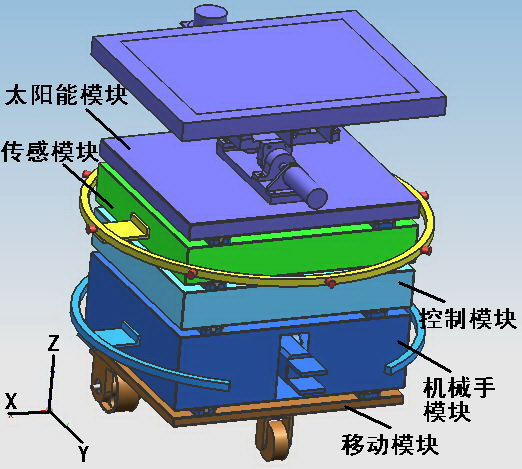
\includegraphics[width=0.35\textwidth]{chap2/Original3DModel.png}}
  \hspace{1in}
  \subfigure[实物图]{
    \label{fig:corereal:b} %% label for second subfigure
    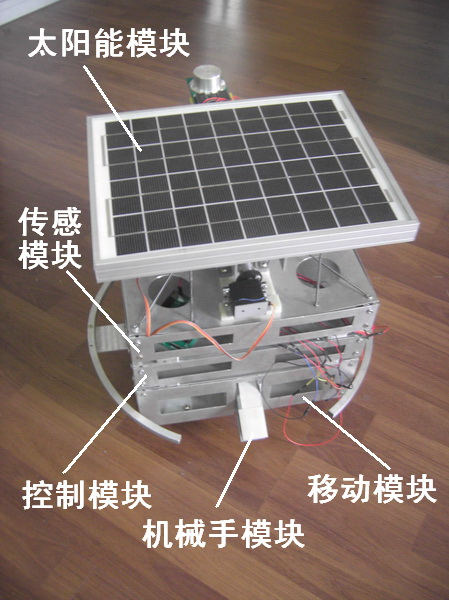
\includegraphics[width=0.35\textwidth]{chap2/OriginalRealModel.PNG}}
  \bicaption[fig.OriginalModel]{原设计方案模型}{原设计方案模型}{Fig}{The Model of the Original Design}
\end{figure}
原机器人的坐标系规定如下:

原点O取为移动模块两驱动轮中心连线的中点,Z轴垂直机器人底面向上,Y轴沿机器人前进方向,X轴由右手定则确定。太阳能驱动模块化机器人结构与坐标方向示意如图\ref{fig:corereal:a} 所示。
\subsection{传感器模块结构}
传感模块主体为立方壳体,模块上、下表面分别安装上、下接口。两侧分别固定一个支架,再在支架上固定一个圆环,在圆环的前、后、左、右及左前、右前、左后、右后的八等分圆处分别安装一个超声波传感器。主要用于实现对八个方位的障碍物探测与测距功能。如图\ref{fig.SensorSupport} 所示。
\begin{figure}[!htp]
  \centering
  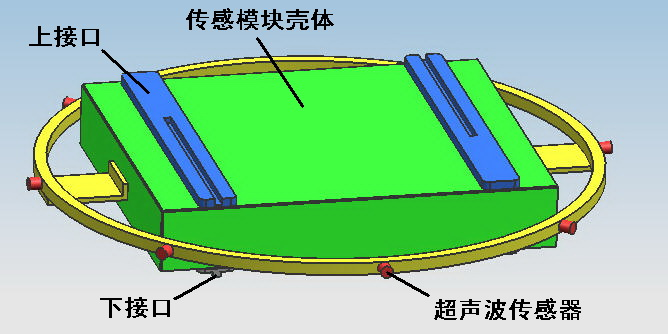
\includegraphics[width=0.8\textwidth]{chap2/OriginalSensorSupport.PNG}
  \bicaption[fig.SensorSupport]{原设计方案传感器支架}{原设计方案传感器支架}{Fig}{The Sensor Stand of Original Design}
\end{figure}
\subsection{控制模块结构}
控制模块主体也为立方壳体,模块上、下表面也分别安装上、下接口。其内安装主控制系统电路板和双轴陀螺仪、电子罗盘等,实现机器人自身的倾角和方位测量等功能,接收传感模块输入的障碍物探测信息,并输出对移动模块和机械手模块的控制信号。如图\ref{fig.CentralUnit} 所示。
\begin{figure}[!htp]
  \centering
  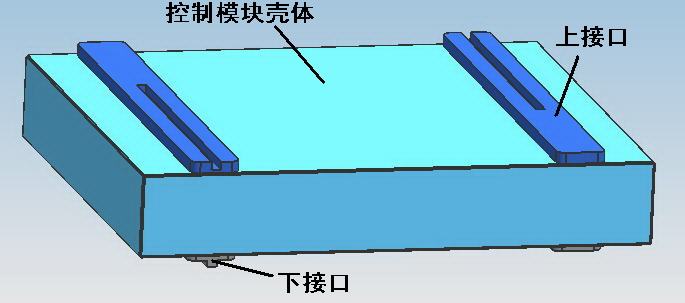
\includegraphics[width=0.8\textwidth]{chap2/OriginalCentralUnit.PNG}
  \bicaption[fig.CentralUnit]{原设计方案控制模块}{原设计方案控制模块}{Fig}{The Control Module of Original Design}
\end{figure}
\subsection{移动模块结构}
移动模块主体为较薄的立方壳体,模块上表面安装上接口,下表面安装两个驱动轮和一个从动脚轮。两个驱动轮分别由一个直流电机带动,利用两驱动轮差速运动实现转向运动;从动脚轮具有两个自由度,在摩擦作用下可以自动适应转动方向;磁珠装于轮轴上,通过安装于底盘上的霍尔传感器输出转速信息给控制模块。如图\ref{fig.ChesisOld} 所示。
\begin{figure}[!htp]
  \centering
  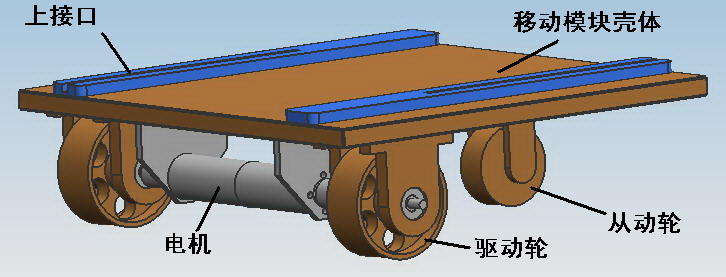
\includegraphics[width=0.8\textwidth]{chap2/OriginalChesis.PNG}
  \bicaption[fig.ChesisOld]{原设计方案移动模块}{原设计方案移动模块}{Fig}{The Mobile Module of Original Design}
\end{figure}
\subsection{标准化机电接口}
原方案设计的接口如图\ref{fig.OriginalPort} 所示。
\begin{figure}
  \centering
  \subfigure[下接口]{
    \label{fig:port:a} %% label for first subfigure
    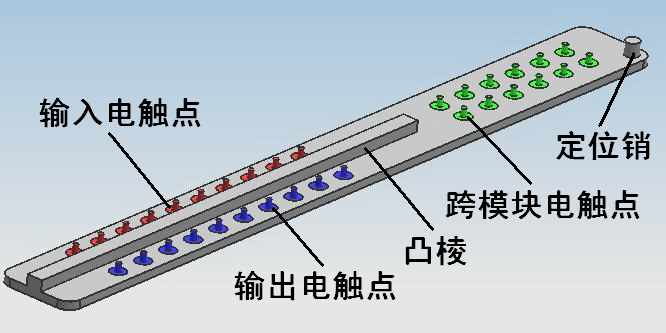
\includegraphics[width=0.4\textwidth]{chap2/OriginalPortUp.png}}
  %\hspace{1in}
  \subfigure[上接口]{
    \label{fig:port:b} %% label for second subfigure
    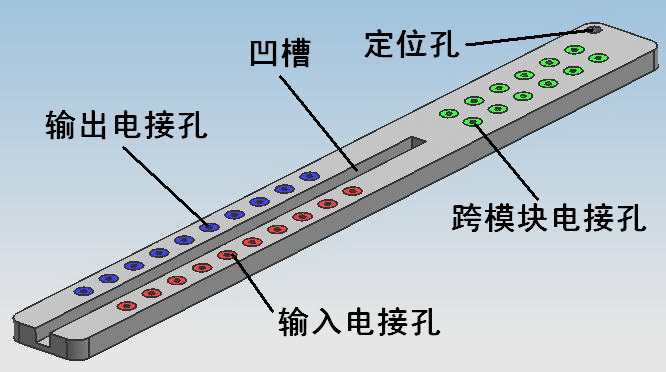
\includegraphics[width=0.4\textwidth]{chap2/OriginalPortDown.PNG}}
  \bicaption[fig.OriginalPort]{原设计方案标准化接口}{原设计方案标准化接口}{Fig}{The Communication Port Original Design}
\end{figure}
对接时,下接口面上的凸棱与上接口面上的凹槽配合,可限制对接的模块在X方向上的滑动自由度,再加上定位销与定位孔的配合,可限制模块沿着凹槽在Y方向上的滑动自由度,而上接口与下接口面配合,可限制垂直模块底面的Z方向上的平移自由度。如此,可方便地进行模块的机械对接。

\section{通用可扩展模块的补充设计}
在新的机器人系统中,将不再采用以前机器人的控制结构。在上面的介绍中,可以获知以前机器人拥有单一控制模块,所有其他模块都由这一单一的模块进行控制。这就要求控制系统在新加入模块时要对总控制模块再编程。而且对于这种设计,为了实现其他模块的功能,不得不将大量的控制接口引出,集成在机械结构上,如上一节标准化机电接口设计所述。这种做法存在众多缺点。首先,接出来的众多接口提高了模块系统的复杂性,这些结构必须以有一定的形式存在于整合机器人个体的各个模块上,但是提供接口的模块却未必会用到接口功能,这就产生了设计资源与加工资源的浪费;其次这种设计缺少灵活性,在新加入功能模块或是主控芯片变动时,需要对接口进行再设计与加工,不利于机器人模块的升级使用;第三机械触点式接口易于磨损,长期使用的可靠性极差。综上所述,本设计提供了一种新的思路去解决上面所述的种种问题。

将对于模块的控制电路集成在各个模块上,即抛弃主控模块的概念,而在各个模块上设置控制电路,是每个模块可以脱离主体进行单独工作。这样只需要一种协调各模块的机制就可以了。现存的多种基于嵌入式系统的通讯机制可以满足这一要求。不过在众多系统中CAN总线系统及协议,是相对最好的解决方案,也是本设计所采用的方案。其有如下优点,第一,CAN总线接线简单,总线中只有CANH和CANL两条线;第二,协议成熟,这一协议的2.0版本是由博世公司于1996年提出的。至今经过了10余年的使用足以证明这个协议的可靠性;三,可靠性高,因为依赖的连线比较少,所以容错率会比SCI,SPI,$I^2C$等其他协议要高;四,可适用于大规模集群网络,就是指可以使众多模块在系统中协同工作。

根据这一思路,对系统进行了设计。关于电路硬件部分的详细说明请见下一章相应部分内容。在本节和下一节将给出根据此思想所设计的通用机械模块和模块间通讯接口的机械设计。

新的模块设计三维立体图如图\ref{fig.NewModuleBody} 所示,用于连接上下两个模块的槽型和凸起机构如图\ref{fig.SlotAndHeave} 所示。其中模块结构包括上下两个交叉的加强筋和一个电路板固定区,以及可以扩展的侧方空间。
\begin{figure}[!htp]
  \centering
  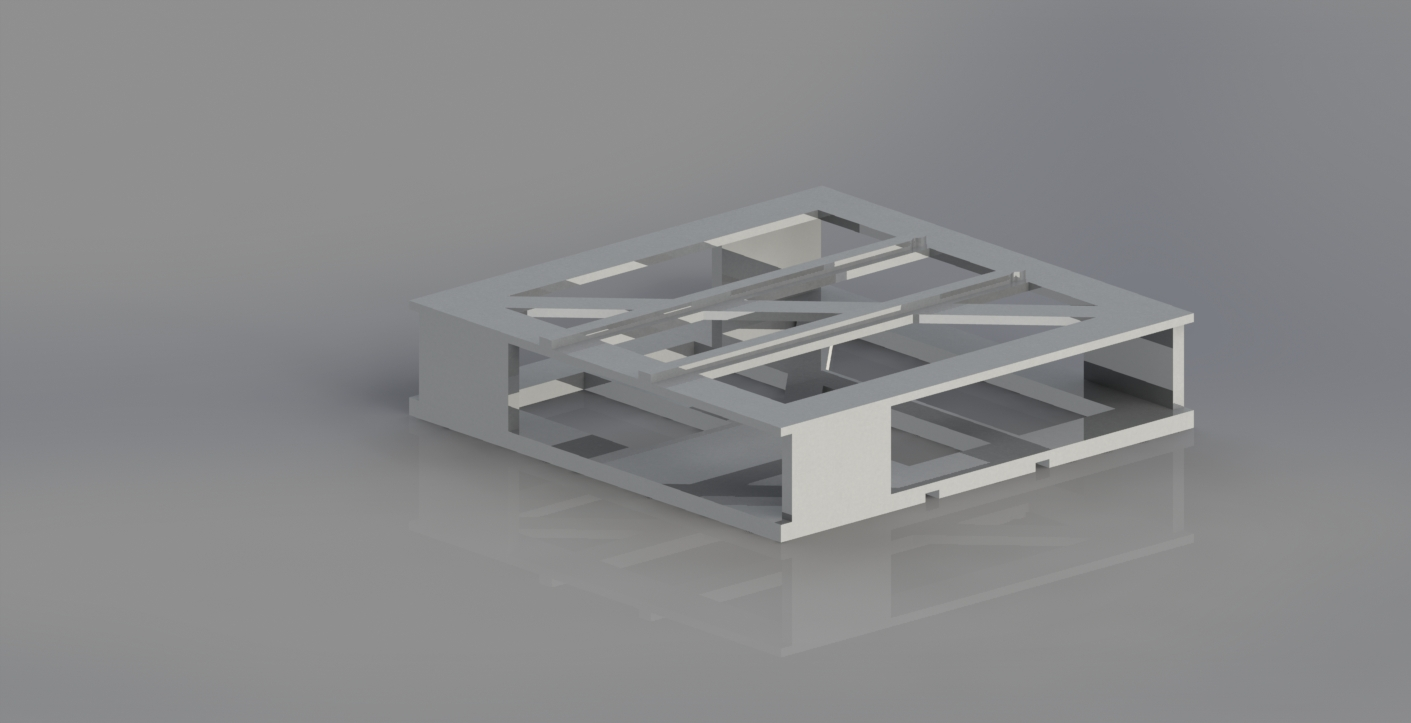
\includegraphics[width=0.8\textwidth]{chap2/NewModel.JPG}
  \bicaption[fig.NewModuleBody]{新设计的通用模块三维立体图}{新设计的通用模块三维立体图}{Fig}{The General Module of New Design}
\end{figure}
\begin{figure}
  \centering
  \subfigure[处于模块上端面的凸起]{
    \label{fig:cnt:a} %% label for first subfigure
    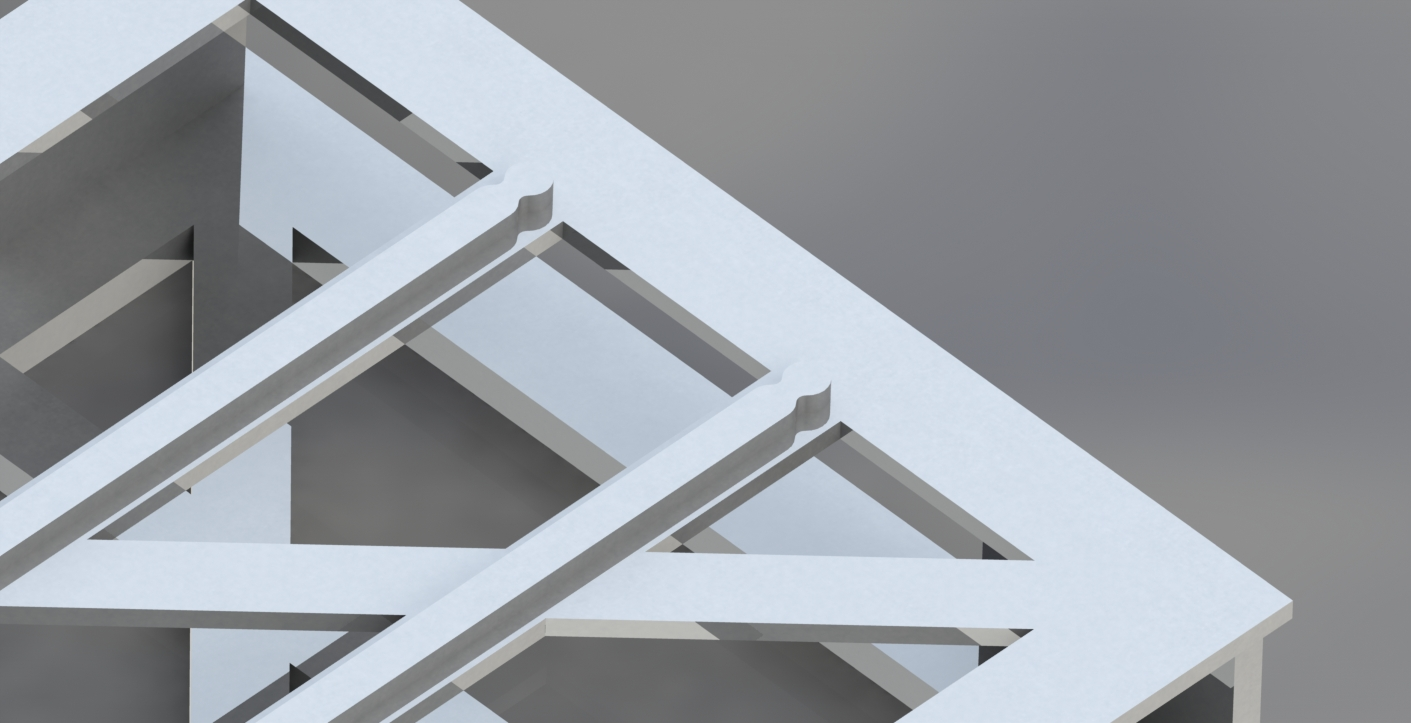
\includegraphics[width=0.4\textwidth]{chap2/LockHead.JPG}}
  %\hspace{1in}
  \subfigure[处于模块下端面的凹槽]{
    \label{fig:cnt:b} %% label for second subfigure
    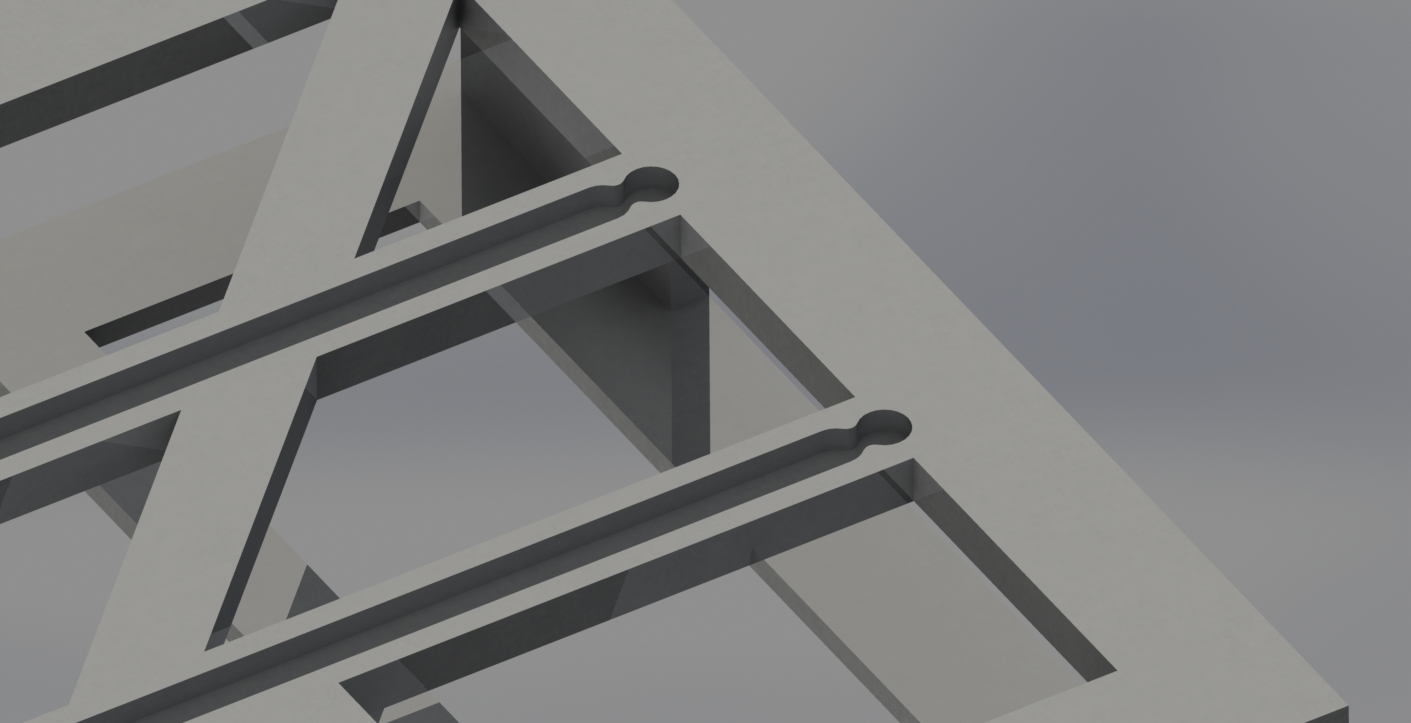
\includegraphics[width=0.4\textwidth]{chap2/LockSlot.JPG}}
  \bicaption[fig.SlotAndHeave]{新设计的通用模块的连接机构}{新设计的通用模块的连接机构}{Fig}{The Connection Structure of the New Design}
\end{figure}
\section{模块间通用接口的设计}
模块间通用接口既是固定在通用模块体上的,实现模块间通讯的接口电路板的机械固定装置。正如前文说明的那样,为了提高稳定性和简化模块结构,本设计决定使用CAN总线作为传输途径。但是又如前文分析的那样,如果采用接触式方案,将极易磨损而使传输变得不可靠。所以这里采用了光学手段,将总线中的高低电平变成红外LED的亮灭,而另一模块则通过一个光敏三极管接收传过来的光信号,并变回电信号传回另一模块的总线中去。因为光敏三极管是一个极其敏感的元件,为了避免不同光源之间的相互干扰,需要使对应的红外LED和光敏三极管处于同一个密封环境,这就需要在设计机械结构上得以实现。关于转换电路的内容会在第三章相应部分进行详细介绍。而接口的机械接口如图\ref{fig.ComuPort}所示,其位于槽和凸起的末端。
\begin{figure}
  \centering
  \subfigure[处于凸起上的接口]{
    \label{fig:Newport:a} %% label for first subfigure
    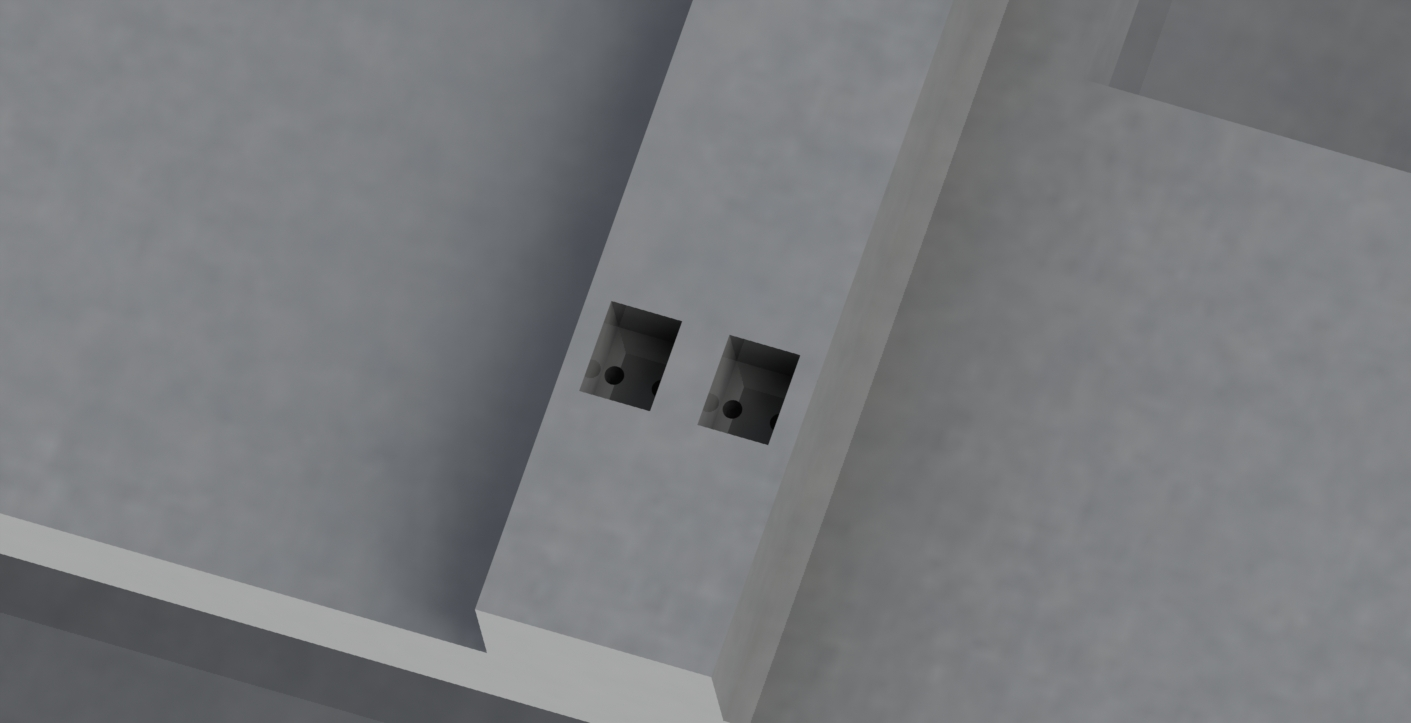
\includegraphics[width=0.4\textwidth]{chap2/PortOnHeave.JPG}}
  %\hspace{1in}
  \subfigure[处于凹槽上的接口]{
    \label{fig:Newport:b} %% label for second subfigure
    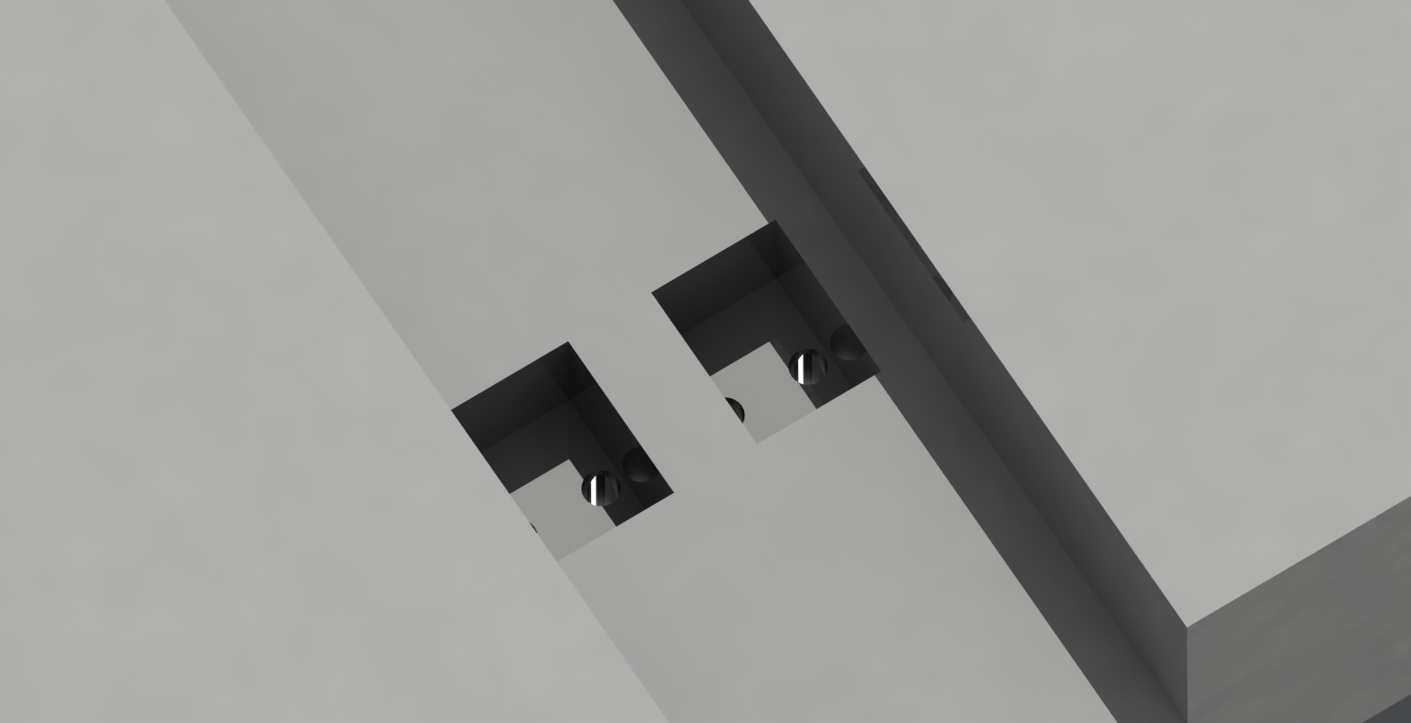
\includegraphics[width=0.4\textwidth]{chap2/PortOnSlot.JPG}}
  \bicaption[fig.ComuPort]{新设计的CAN总线接口}{新设计的CAN总线接口}{Fig}{The Communication Port of the New Design}
\end{figure}
\section{超声波传感器支架的设计}
因为定位的原因,本设计对传感器支架进行了重新设计。虽然圆形的传感器排布可以实现对环境的较好的检测,但是对于计算车体相对于障碍物的相对位置却变得非常复杂。为了解决这一问题,本设计重新对传感器的位置进行了安排。先前的设计文献中只把传感器作为圆柱处理,这显然是不现实的,在这里本设计对传感器尺寸进行了仔细测量,并按实际尺寸画出了传感器对于传感器支架的安装位置。其设计图如图所\ref{fig.NewSensorSupport}示。图中为传感器模块一侧传感器支架的样子,在模块的是个边上各有一个支架,每个支架上有三个超声波传感器。
\begin{figure}[!htp]
  \centering
  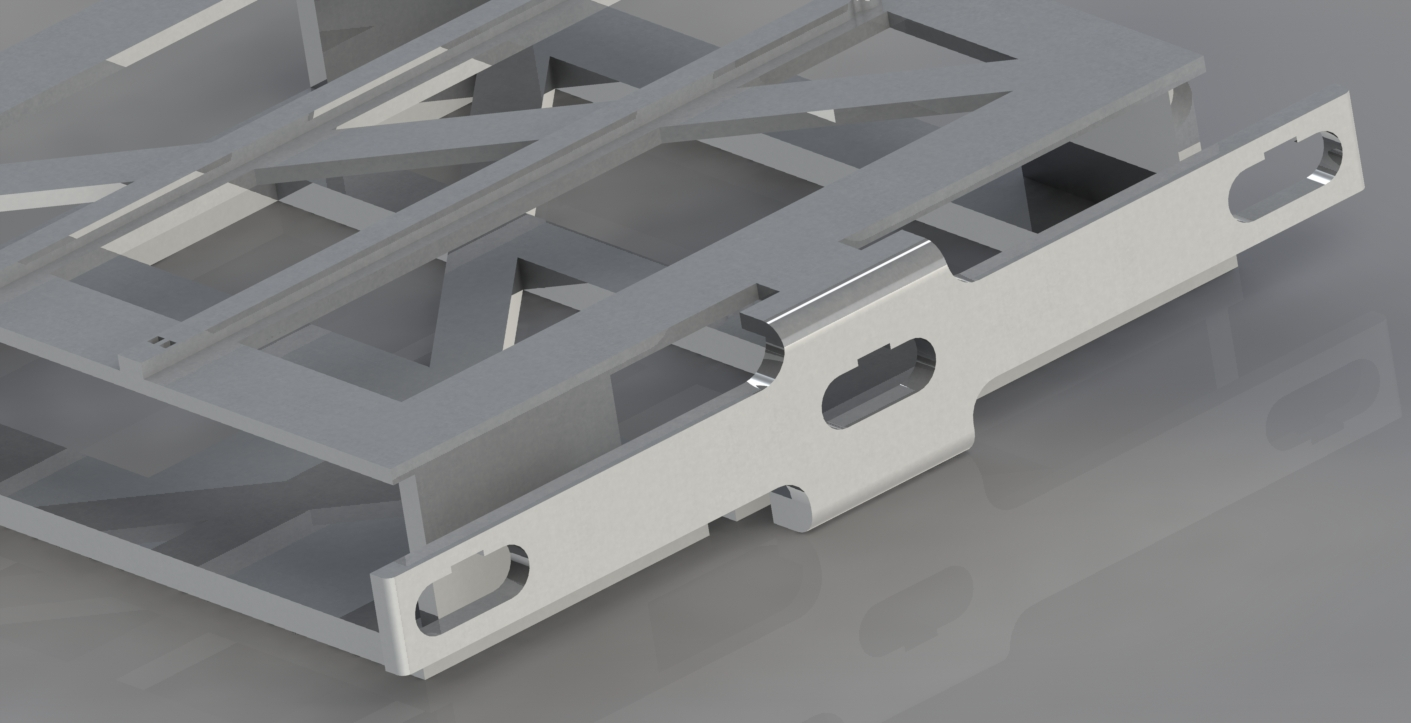
\includegraphics[width=0.8\textwidth]{chap2/SensorSupport.JPG}
  \bicaption[fig.NewSensorSupport]{新设计的传感器支架三维立体图}{新设计的传感器支架三维立体图}{Fig}{The General Module of Sensor Stand}
\end{figure}
\section{底盘编码轮的设计}
最直观的的对于二维坐标的测量莫过于直接测量车体在二维坐标中的的位移。在传统的方法中,我们一般会在电机驱动轴上加装编码器,这样通过测量轮子转过的圈数,在已知轮直径的基础上可以算出每一个轮子走过的路程,再通过车体尺寸等其他参数,可以计算出车体的轨迹,从而得到车体的定位信息。但实际上,这种方法存在着一些问题。首先驱动轮是非常容易打滑的,所以将编码器装到驱动轮上,经过积分后,计算值与实际值之间的误差会发散,得不到准确的坐标值;其次,编码器放在轮子处在好多时候都会增加对于车体轨迹的计算的复杂性。综上所述,如果想使用这种直接的方法对车体进行定位,必须要克服上述诸多的问题。

在本设计中,将编码器独立出来,放置到可以自由安放在底盘某一部位上的从动轮机构上,以实现编码器与主动轮的脱离。因为编码轮可以放置在机器人底盘的任意位置上,所以可以很容易解决计算复杂性的问题。接下来需要解决的就是打滑问题。对于主动轮,打滑的原因是因为电机输出扭矩与地面提供摩擦力不匹配造成的。而因为从动轮没有扭矩输出,所以只需要使地面提供用于克服转轴处摩擦转矩的力就可以了。对摩擦力的要求相对较小。而为了提供足够的摩擦力,只需要施加适当的正压力就可以了。所以这一独立的轮式编码单元必须是弹性结构,可以适应高低欺负的地形,同时可以提供对地面足够的正压力。想要做到这点,就一定要使用弹簧和连杆机构。基于这一准则,本文设计了一个基于四连杆机构的弹性轮式独立编码系统,如图所示。其中蓝色的轮子为万向轮,用来减少对于车体控制的影响。因为难以绘制,所以在这里以普通轮子表示。一段比较长的轮轴上固定光学编码器,因为关于编码器固定的设计比较常见,所以在这里没有画出。
\begin{figure}[!htp]
  \centering
  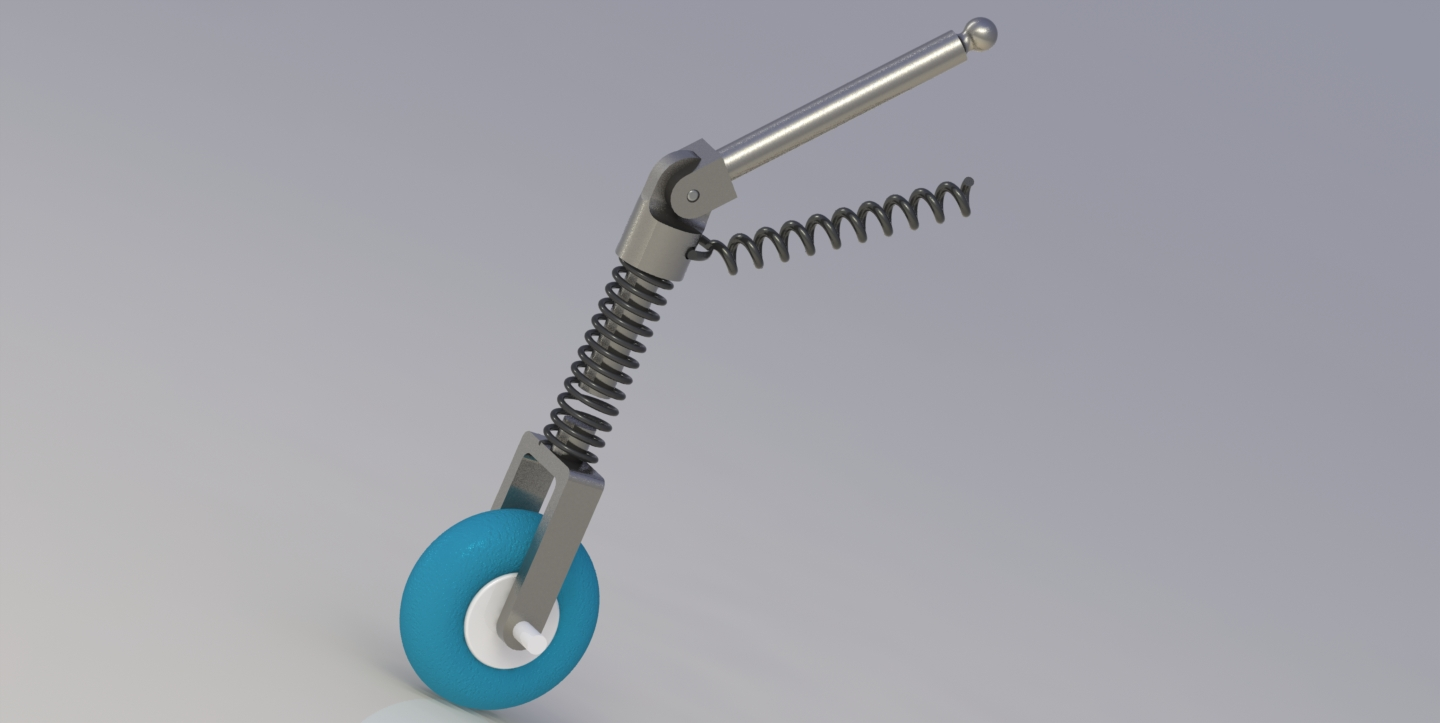
\includegraphics[width=0.8\textwidth]{chap2/EncoderWheel.JPG}
  \bicaption[fig.NewSensorSupport]{新设计的底盘编码轮三维立体图}{新设计的底盘编码轮三维立体图}{Fig}{The General Module of Independent Passive Wheel Encoder}
\end{figure}
\section{本章小结}
本章由已有的机器人设计出发,分析了以前设计的特点,并对设计中的不妥提出了疑问。再根据这些疑问出发,着手改进原来的设计方案。在本章中,详细的介绍了对于通用模块,传感器支架,模块连接机构,模块间传输单元机构和独立轮式编码单元的新的设计方案。通过新旧方案的对比,可以较为容易的 发现,新的设计方案在根本上克服了以前设计方案所存在的问题。

%%==================================================
%% chapter03.tex for SJTU Bachelor Thesis
%% version: 0.5.2
%% Encoding: UTF-8
%%==================================================

% \bibliographystyle{sjtu2} %[此处用于每章都生产参考文献]

\chapter{通用控制电路设计}
\label{chap:electricalSystem}
模块化机器人的各个模块都是可以独立工作的个体。从上一章的设计可知,每个模块都有一个核心板载系统来对本模块的基本功能进行控制。这一设计思路在其它模块化机器人上也有所体现。例如美国加州大学戴维斯分校的Graham G. Ryland等人\upcite{ryland2010design}设计的模块化机器人系统,每个模块是包含四个自由度的可以独立控制并运动的个体。而个体之间通过通信和协议来完成作为组合的总体所实现的功能。在本设计中,因为每个模块都有不同的功能,进行拼装后的实体的机器人通过协同来实现全部功能。为了使设计的硬件能在最大程度上实行公用,本设计将机器人电路进行拆分,并对电路实现了模块化。

每个机器人模块都将实现作为一个模块的基本功能,如实现与其他模块的通信;单独的程序上传与下载、与在线调试;对于自身模块的电源管理;与外部其他系统的通讯;简单的片上调试按钮和指示用数码管和LED。据此本方案设计了每个模块都要使用的通用模块控制电路。而对于不同模块的不同功能需求,本方案设计了大量的外设电路,每一个模块将会在功能性外设及接口设计部分进行讨论与说明。这样的好处是是每一个模块都拥有其工作所用的资源而不会有资源的浪费。例如,用于定位的IMU模块只有地盘模块需要使用。而上层实现其他功能的模块,如机械手并不需要使用,这里没有把其集成在通用板上,是极大的避免了资源的浪费。为了能够使用这些外设电路,本设计已经将片上所有资源系数引出。这样做同时还可供未来通用板的扩展。

一下各小结、节将对整个机器人系统的电路系统进行详细阐述。

\section{通用模块控制电路}
通用电路板本着简单,稳定,可以快速开发和方便部署的原则进行了设计。控制芯片选用了引脚众多,功能强大和文档完善的Freescale公司的MC9S12XS128单片机。本设计使用的是拥有112个引脚的版本。这款芯片的特点是低功耗、高集成、易于扩展,自带看门狗计数器、PWM输出、增强型捕捉定时器\upcite{xn2012baseon}。在本设计中,将通用控制电路板分为两个部分,一个部分是包含BWM程序烧写在线调试器,复位按键和单片机芯片的最小系统;另一部分是提供通用电路功能的接口板。这样设计而不是直接将单片机焊接在接口板上的原因是,一旦单片机烧毁,可以同过更换最小系统来是电路板恢复使用,而不用丢弃整个电路板,基板上昂贵芯片。

下面的部分将对这两个模块进行详细的介绍。

\subsection{最小系统}
最小系统的电路图如图\ref{fig.CoreSch} 所示。最小系统实物图如图\ref{fig.CorePhoto} 所示。 \\
\begin{figure}[!htp]\label{fig.CorePhoto}
  \centering
  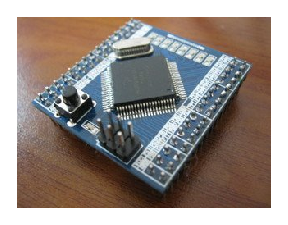
\includegraphics{chap3/coreminsys.eps}
  \bicaption{最小系统实物图}{最小系统实物图}{Fig}{the Minimal Core System}
\end{figure}
\begin{figure}[!htp]\label{fig.CoreSch}
  \centering
  \bicaption{最小系统电路图}{最小系统电路图}{Fig}{Schematic of the Minimal Core System}
  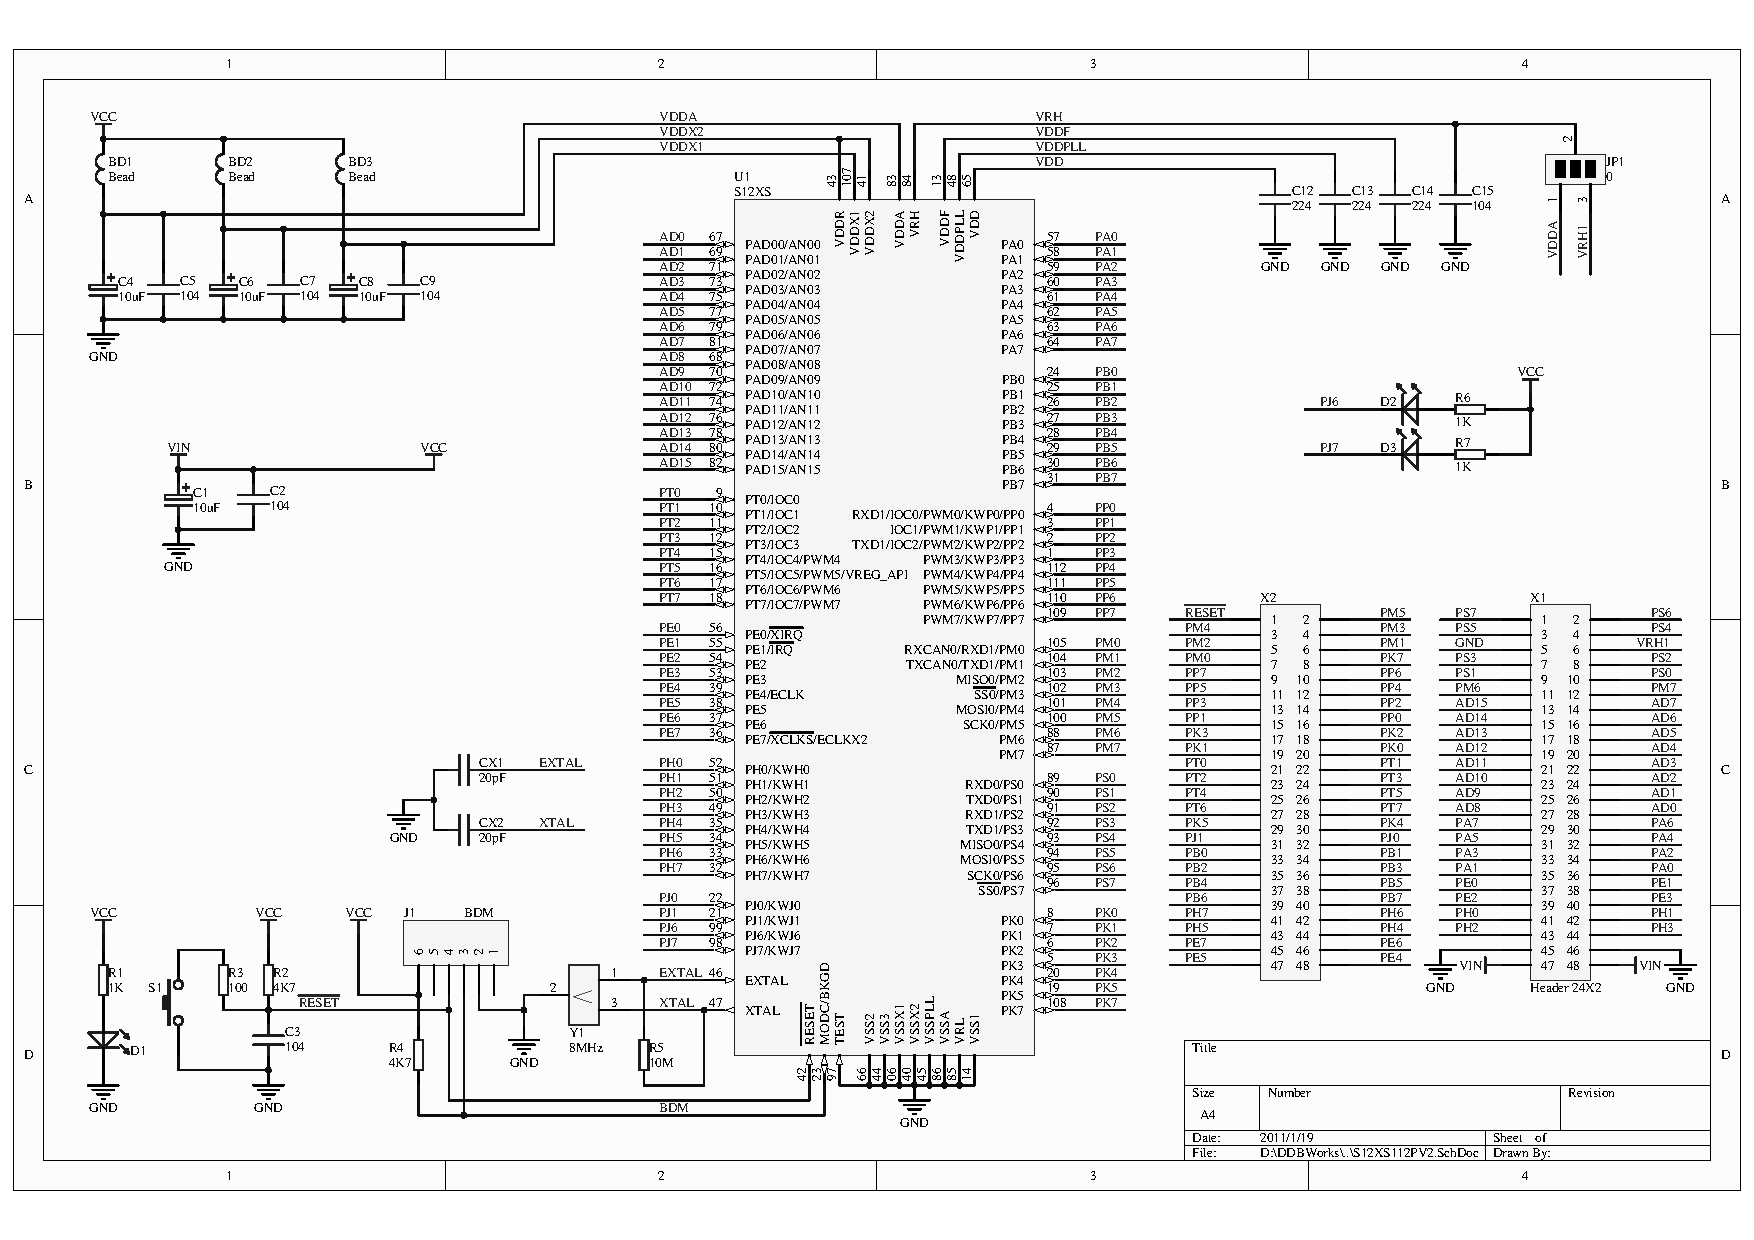
\includegraphics[angle=-90,width=1.3\textwidth]{chap3/Core112V2.pdf}
\end{figure}

这块最小系统板上有一个16MHz的晶振连接至芯片。芯片正常工作时的频率是由锁相环(PLL)超频到40MHz的。这块最小系统还有一个复位键,引入芯片RESET引脚,将检测电路的下降沿进行复位。同时最小系统上海提供一个BWM程序上传和下载及在线调试模块。片上提供128k片上RAM,可以用来储存芯片执行用程序。还有一个独立的电源管理模块,以提供稳定的5v电压给单片机工作。之所以称为最小系统,就是因为以上是这块芯片的全部功能元件。如原理图所示,这块最小系统的其他功能就是简单的将单片机所有引脚引出。 

\subsection{功能接口板}
功能接口板是通用模块控制电路的核心部分。它具有承上启下的作用,得到最小系统引出的单片机全部空余引脚,并对其功能进行设计。其电路图如图\ref{fig.BaseSch} 所示。 其共分为电源管理,CAN总线,单片机接口,电压测试单元,串口通讯,数码管显示单元,LED及案件阵列和引出接口几部分。 
\begin{figure}[!htp]\label{fig.BaseSch}
  \centering
  \bicaption{功能接口板电路图}{功能接口板电路图}{Fig}{Schematic of Base Board}
  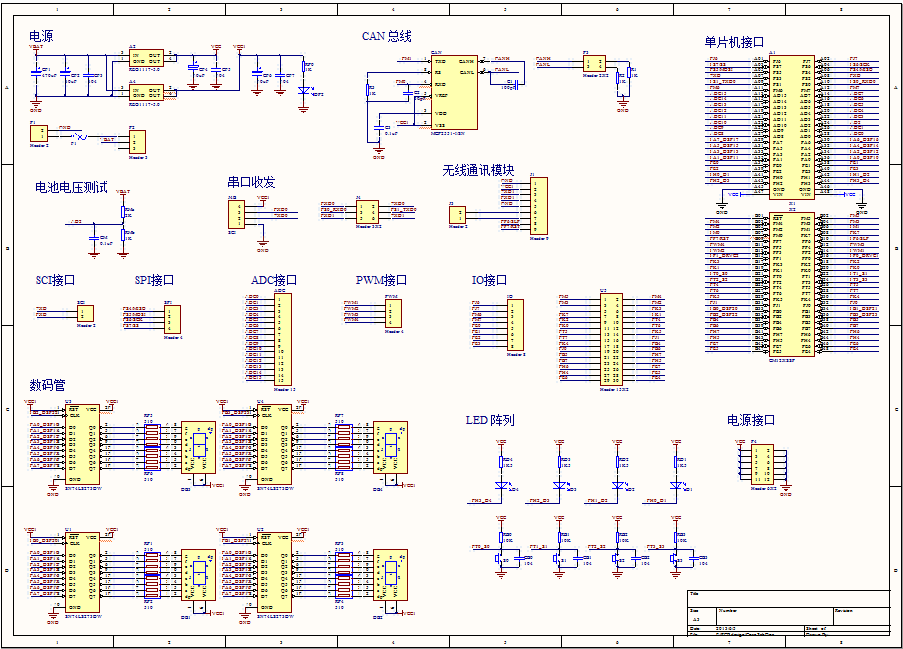
\includegraphics[angle=-90,width=0.8\textwidth]{chap3/CoreBoardSchematic.PNG}
\end{figure}


其中电源管理部分的电路如图\ref{fig.BaseScrMg}。使用两片1117输出两个5v电压,为了使电流相差较大模块之间不会相互干扰。其中一个给单片机及通讯模块供压,电流小,对电流稳定性要求高;而另一路主要给外设电路供压。 
\begin{figure}[!htp]\label{fig.BaseScrMg}
  \centering
  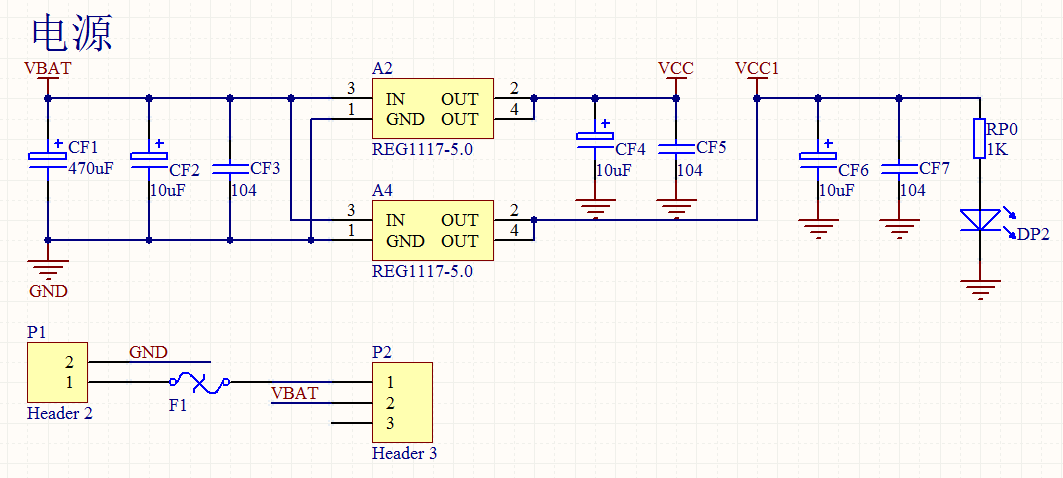
\includegraphics[width=0.8\textwidth]{chap3/CoreBoardPowerMg.PNG}
  \bicaption{电源管理电路原理图}{电源管理电路原理图}{Fig}{Schematic of Power Source Management Unit}
\end{figure}


CAN总线电路图如图所示\ref{fig.BaseCAN} 。用一块Microchip公司生产的MCP2511作为单片机内置CAN模块的Transceiver,将CAN端口数据打包编码后传输到总线中去。前面已经介绍过了这款机器人将打破传统的接触式传输连线,而是使用光学方法进行数据传输,其中这里CAN中线的输出口,就是要连接到光学传输接口板上。
\begin{figure}[!htp]\label{fig.BaseCAN}
  \centering
  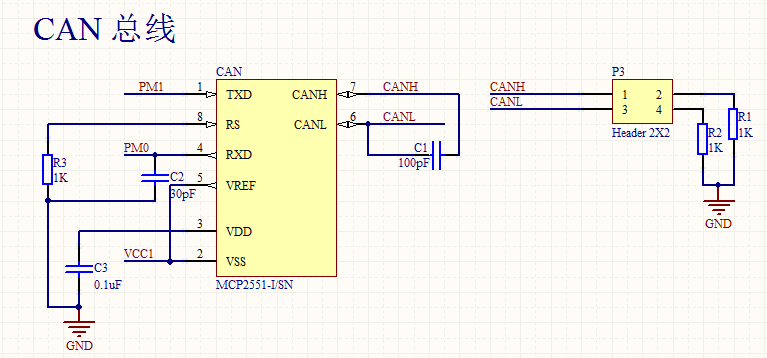
\includegraphics[width=0.8\textwidth]{chap3/CoreBoardCANBus.PNG}
  \bicaption{CAN电路原理图}{CAN电路原理图}{Fig}{Schematic of CAN Bus Unit}
\end{figure}


CAN总线2.0协议\upcite{bosch1991can}是由博世公司提出被提供支持的。因为其两线制的机制,和可以同时连接非常多个模块,并能组织各个节点模块共同工作的特点二大量应用在汽车领域。其传输速度快,稳定性强的特点也为其能轻松移植到机器人系统中来提供了可行性。相对较少的接线同时也意味着极大的容错率,这就是本设计选择CAN总线最为模块间传输工具的原因。这一设计的灵感来源于Ying Zhang等人\upcite{zhang2002massively}的研究。

功能接口板的PCB设计图如图\ref{fig.CorePCB} 所示。其虚拟实物图如图\ref{fig.CoreReal} 所示,3D立体仿真图如图\ref{fig.Core3D} 所示。 
\begin{figure}\label{fig.CorePCB}
  \centering
  \subfigure[PCB正面]{
    \label{fig:corepcb:a} %% label for first subfigure
    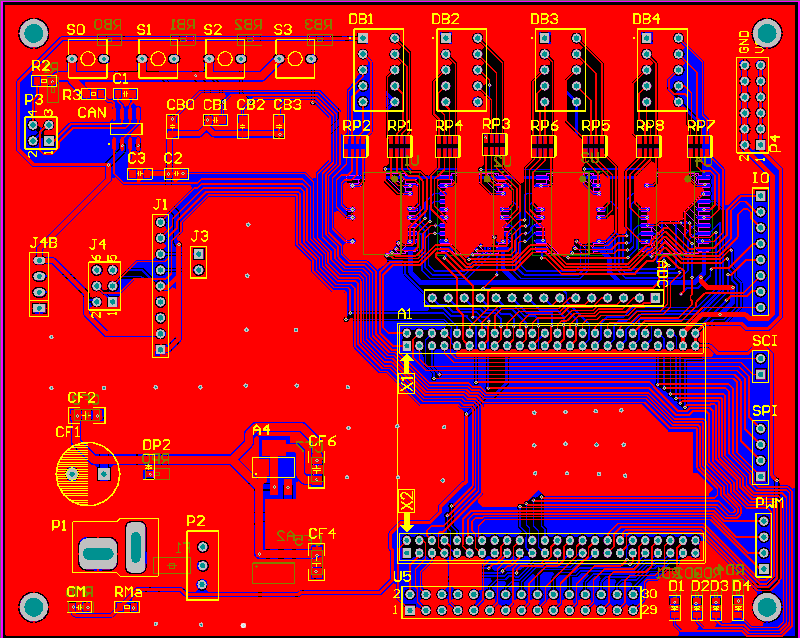
\includegraphics[width=0.35\textwidth]{chap3/CoreBoardTop.PNG}}
  \hspace{1in}
  \subfigure[PCB背面]{
    \label{fig:corepcb:b} %% label for second subfigure
    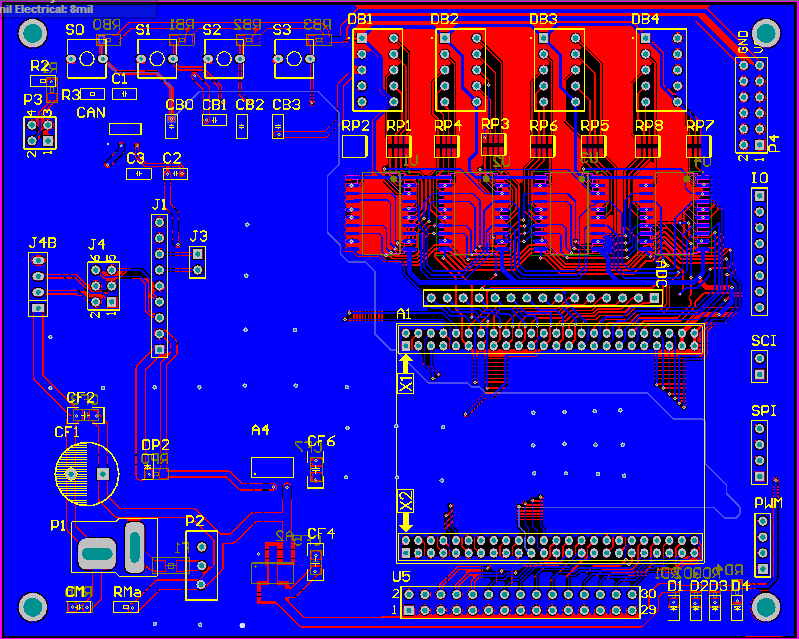
\includegraphics[width=0.35\textwidth]{chap3/CoreBoardBottom.PNG}}
  \bicaption{功能接口板的设计PCB样图}{功能接口板的设计PCB样图}{Fig}{The PCB View of Main Base Board}
\end{figure}
\begin{figure}\label{fig.CoreReal}
  \centering
  \subfigure[PCB正面]{
    \label{fig:corereal:a} %% label for first subfigure
    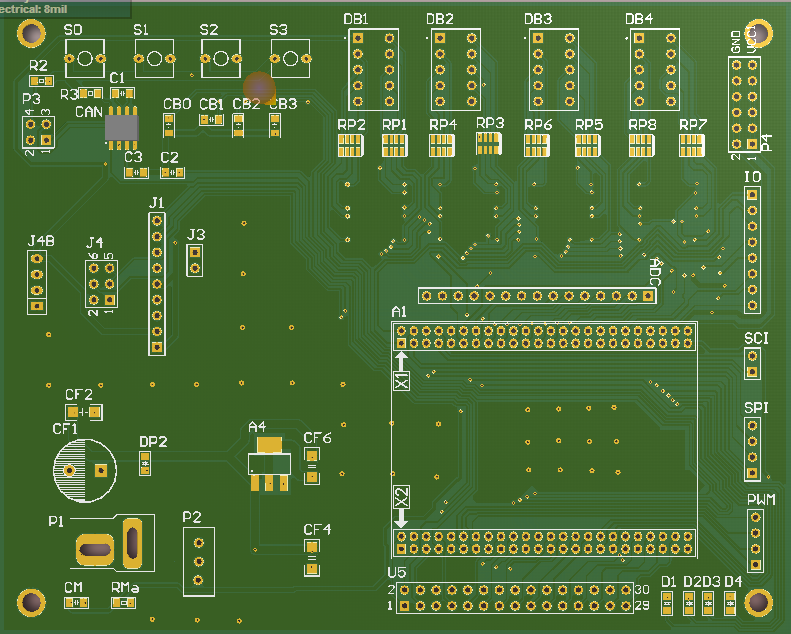
\includegraphics[width=0.35\textwidth]{chap3/CoreBoardManTop.PNG}}
  \hspace{1in}
  \subfigure[PCB背面]{
    \label{fig:corereal:b} %% label for second subfigure
    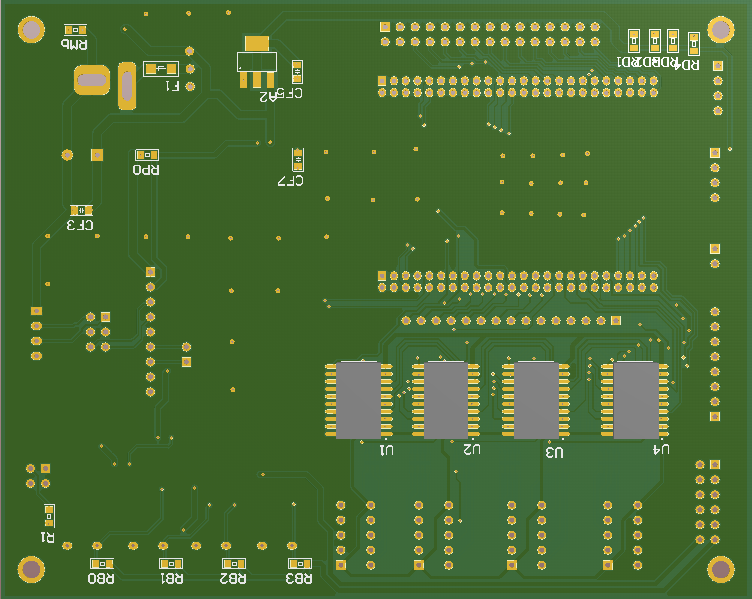
\includegraphics[width=0.35\textwidth]{chap3/CoreBoardManBottom.PNG}}
  \bicaption{功能接口板的虚拟实物图}{功能接口板的虚拟实物图}{Fig}{The Virtual View of Main Base Board}
\end{figure}
\begin{figure}[!htp]\label{fig.Core3D}
  \centering
  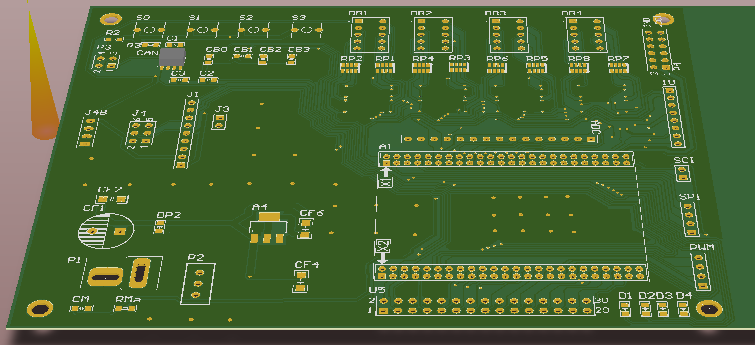
\includegraphics[width=0.8\textwidth]{chap3/CoreBoard3D.PNG}
  \bicaption{功能接口板的虚拟实物图3D}{功能接口板的虚拟实物图3D}{Fig}{The 3D Virtual View of Main Base Board}
\end{figure}
\section{功能型外设及接口设计}
功能性外设主要提供某个模块所需要的独特功能。这些模块可能包括机器人应用中的方方面面。如无线通讯模块:用来是摸个机器人模块与外部设备,如远程计算通讯,从而实现信息的沟通或是机器人于远程系统的交互;舵机驱动模块:可以用来驱动具有多舵机结构的机械臂或其他的多舵机应用模块;IMU和GPS模块:用来实现定位,机器人姿态探测等功能;电机驱动模块,用来驱动电机,可以用在轮式底盘或是履带式底盘的驱动;编码器模块:可以用来对固定于某一电机或伺服电机舵机上的编码器进行驱动与计数;传感器模块:用来驱动传感器来对外部信息进行采集和处理;以及其他应用领域的模块等等。本设计因为只对移动平台进行了设计及研究,所以只具体设计了IMU模块,电机驱动模块,编码器模块,传感器模块和光电CAN传输模块。对于每一个模块的详细设计如下。

\subsection{IMU模块}
IMU是Inertial measurement unit(惯性测量单元)的缩写。本方案所设计的IMU包括传统的加速度计和陀螺仪,同时参考了Minor等人\upcite{minor2001utilization}的设计,在模块中引入了磁倾角传感器(电子罗盘)。在这一模块的设计中,使用了一片SCA100T两轴角速度传感器,用来采集平行于地面的平面内的加速度;一个ZCC212N电子罗盘封装单元,这一单元将测得的与地磁场倾角数据通过SCI协议传输回单片机进行处理;以及一个LYPR540三轴陀螺仪,用以测量角加速度。电路设计原理图如图\ref{fig.IMUSch} 所示,PCB设计样图如图\ref{fig.IMUPCB} 所示,虚拟实物图如图\ref{fig.IMUReal} 所示。 
\begin{figure}[!htp]\label{fig.IMUSch}
  \centering
  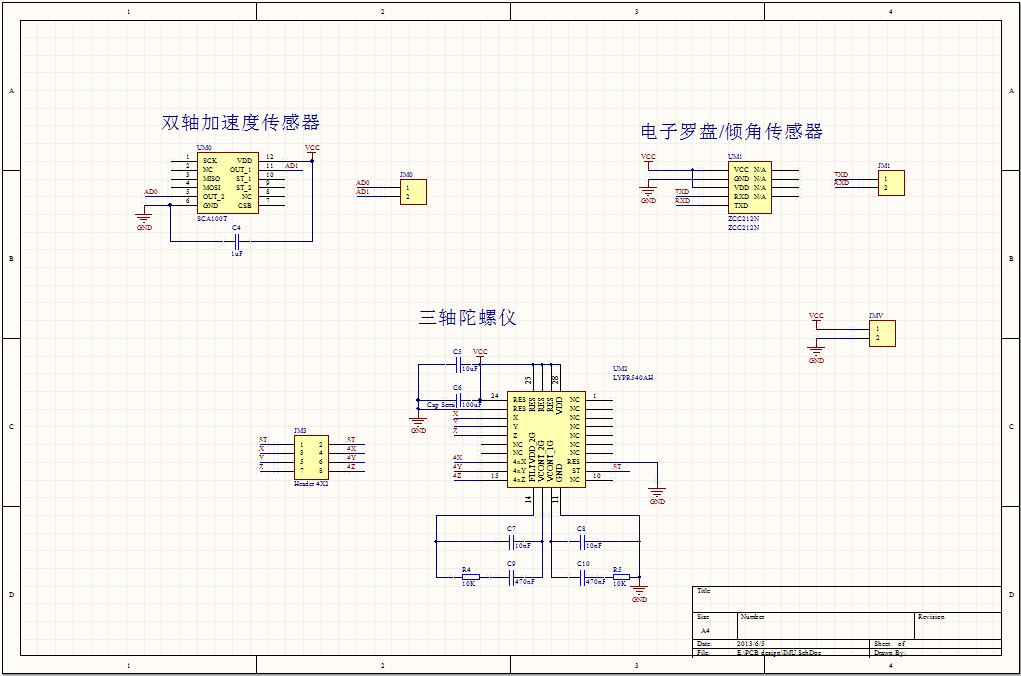
\includegraphics[angle=-90,width=0.8\textwidth]{chap3/IMU.PNG}
  \bicaption{IMU电路原理图}{IMU电路原理图}{Fig}{Schematic of IMU Unit}
\end{figure}
\begin{figure}\label{fig.IMUPCB}
  \centering
  \subfigure[PCB正面]{
    \label{fig:corepcb:a} %% label for first subfigure
    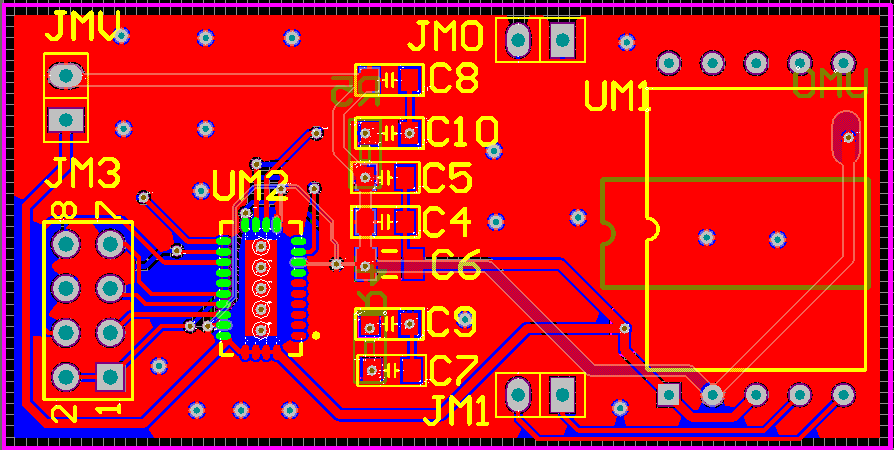
\includegraphics[width=0.35\textwidth]{chap3/IMUfront.PNG}}
  \hspace{1in}
  \subfigure[PCB背面]{
    \label{fig:corepcb:b} %% label for second subfigure
    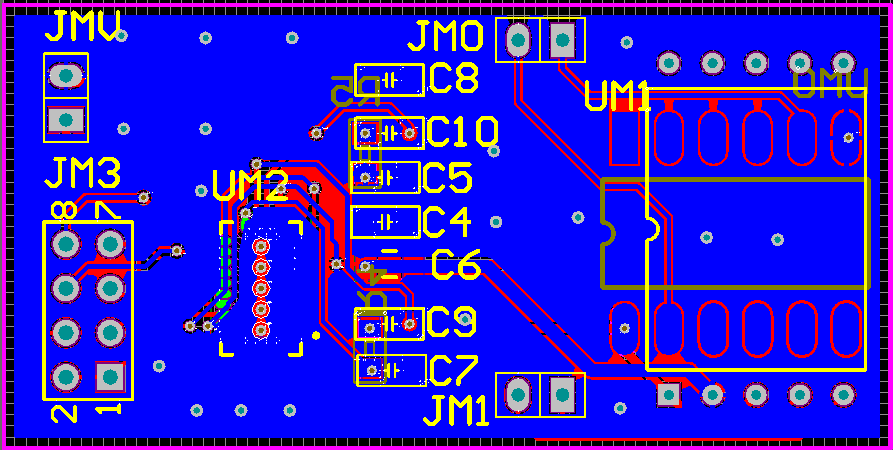
\includegraphics[width=0.35\textwidth]{chap3/IMUback.PNG}}
  \bicaption{IMU的设计PCB样图}{IMU的设计PCB样图}{Fig}{The PCB View of IMU}
\end{figure}
\begin{figure}\label{fig.IMUReal}
  \centering
  \subfigure[PCB正面]{
    \label{fig:corereal:a} %% label for first subfigure
    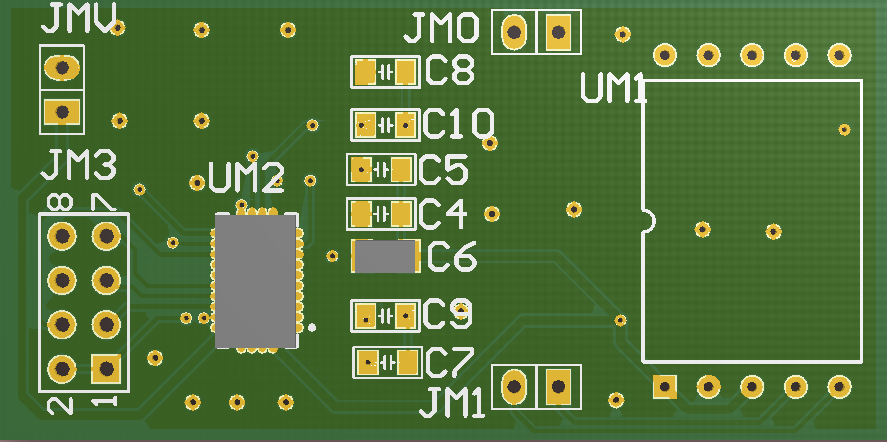
\includegraphics[width=0.35\textwidth]{chap3/IMUfrontVr.PNG}}
  \hspace{1in}
  \subfigure[PCB背面]{
    \label{fig:corereal:b} %% label for second subfigure
    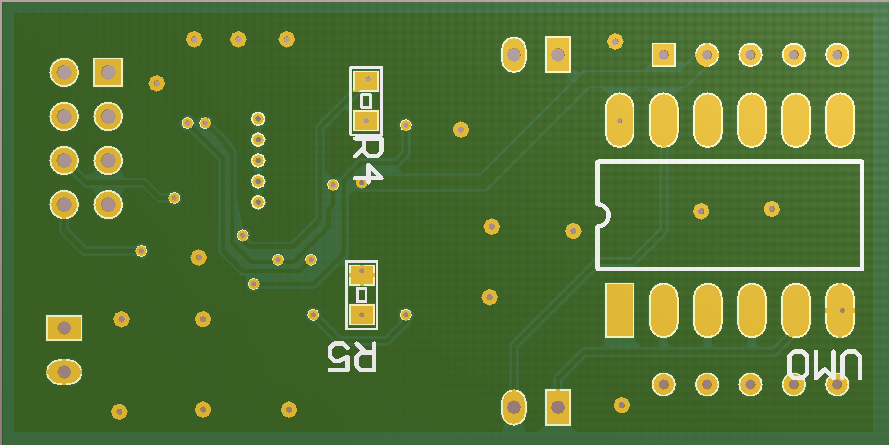
\includegraphics[width=0.35\textwidth]{chap3/IMUbackVr.PNG}}
  \bicaption{IMU的虚拟实物图}{IMU的虚拟实物图}{Fig}{The Virtual View of IMU}
\end{figure}

\subsection{驱动模块}
电机驱动模块,采用传统的H桥式电路。其电路原理简图如图\ref{fig.DrvPrinciple} 所示。 
\begin{figure}[!htp]\label{fig.DrvPrinciple}
  \centering
	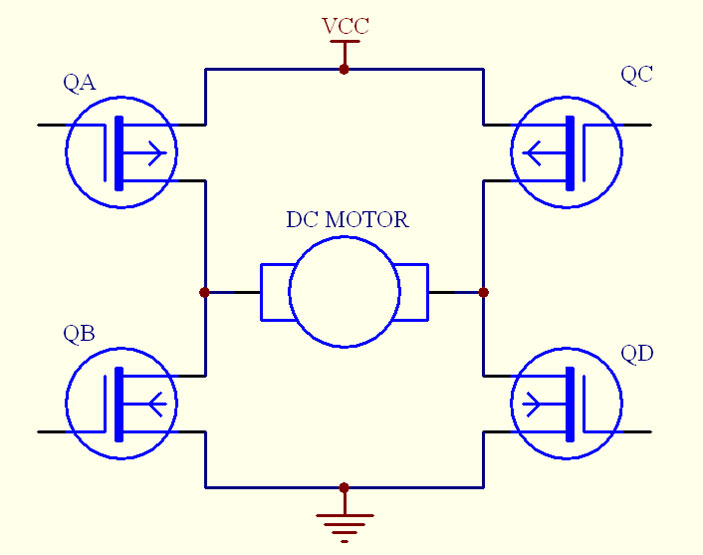
\includegraphics[width=0.3\textwidth]{chap3/H_Bridge.jpg}
	\bicaption{H桥电路原理简图}{H桥电路原理简图}{Fig}{H Bridge}
\end{figure}


其工作原理为,对角线上的MOSEFET或是BJT同时断开和闭合,相邻的两个MOSFET和BJT不同时断开和闭合。从而达到是电流可以以不同方向经过电机,而使电机可以正转或反转。现在有多种集成的桥式电路芯片可供选择,而不必用MOSFET自行搭建H桥式电路。这种集成芯片有多种好处,比如稳定性高,紧凑所占空间小,简化电路设计等。所以本方案的驱动电路是直接基于BTS7960这款H桥式芯片设计的。同时电机需要使用PWM脉冲调制器产生方波来进行控速,通过改变方波的占空比来改变作用在电机上的等效电压来实现调速。其原理图如图\ref{fig.Drv} 所示,PCB设计样图如图\ref{fig.DrvPCB} 所示。
\begin{figure}[!htp]\label{fig.Drv}
  \centering
  \bicaption{驱动电路电路图}{驱动电路电路图}{Fig}{Schematic of Driver Board}
  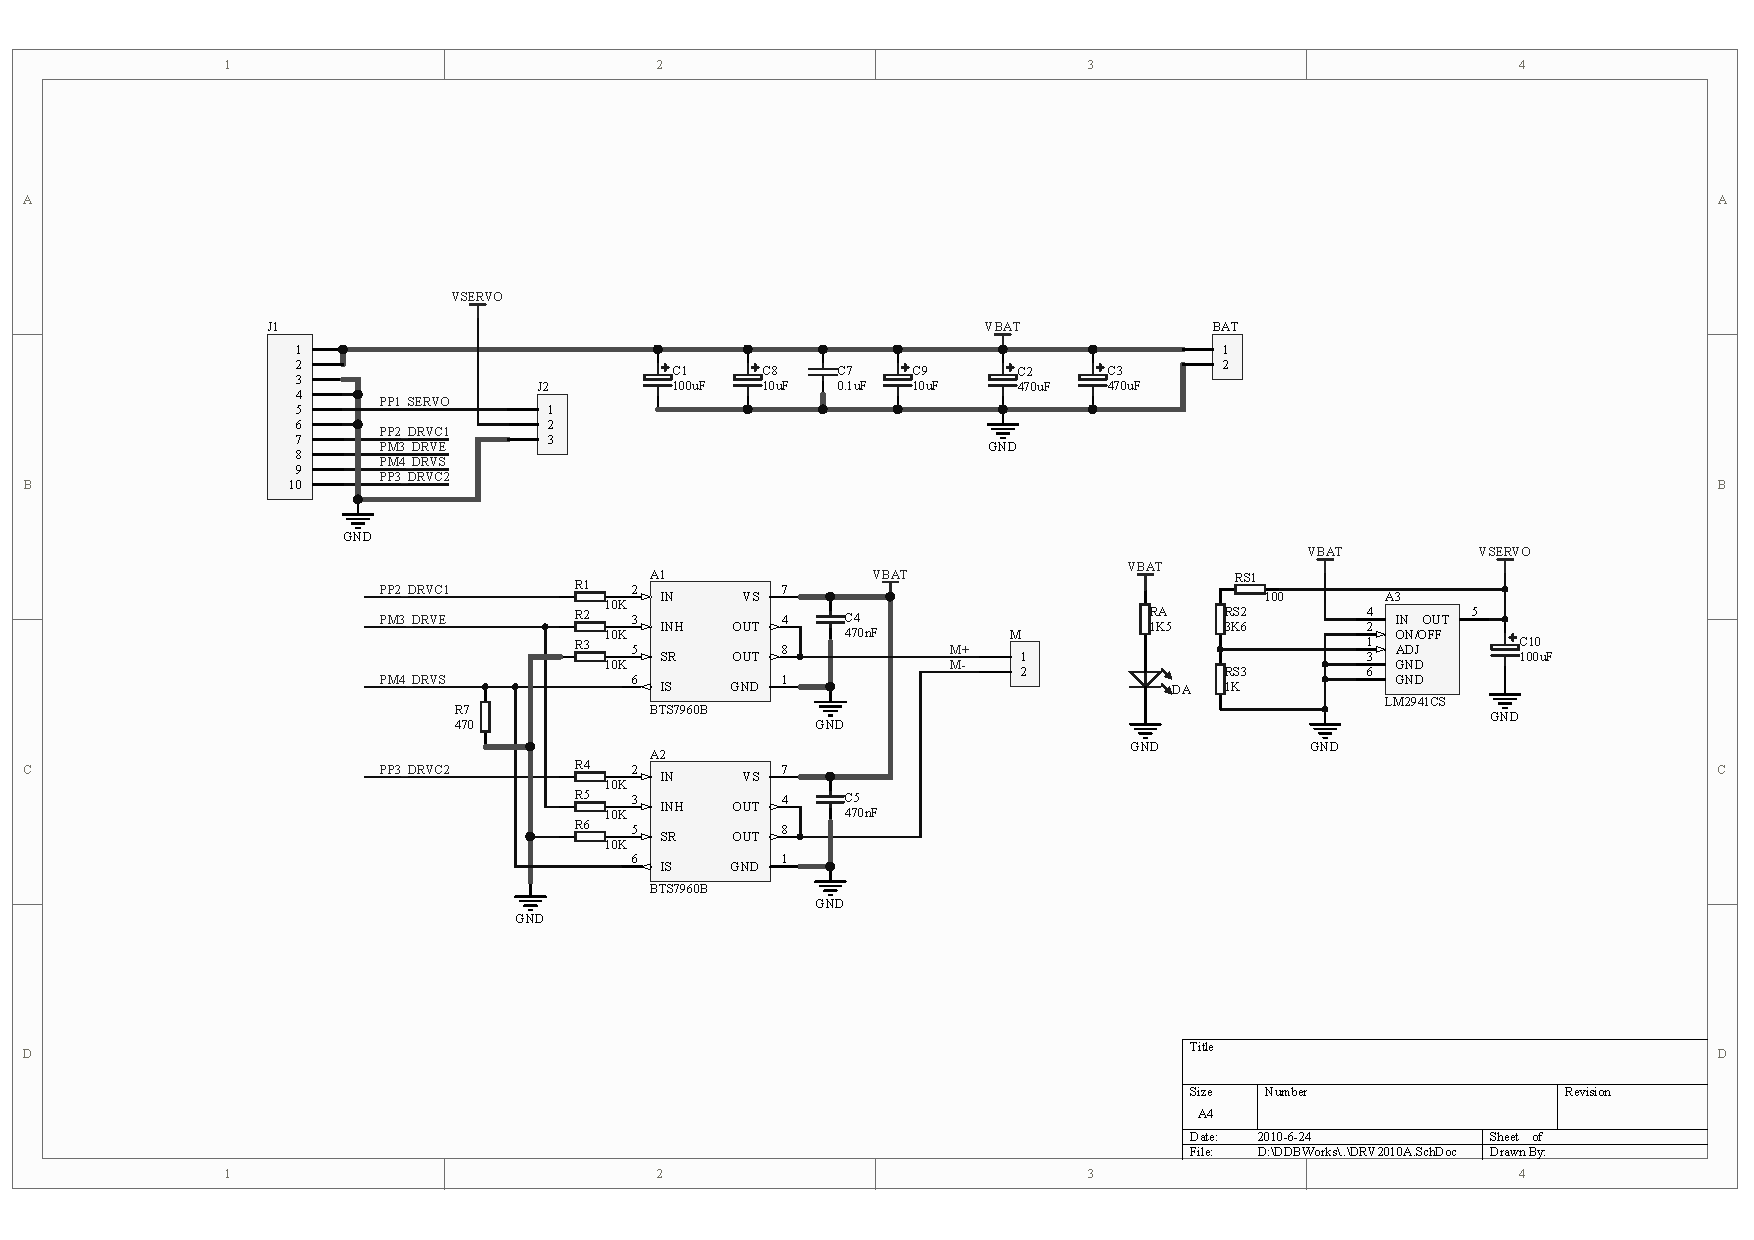
\includegraphics[angle=-90,width=0.8\textwidth]{chap3/DRV2010A.pdf}
\end{figure}
\begin{figure}\label{fig.DrvPCB}
  \centering
  \subfigure[PCB正面]{
    \label{fig:corepcb:a} %% label for first subfigure
    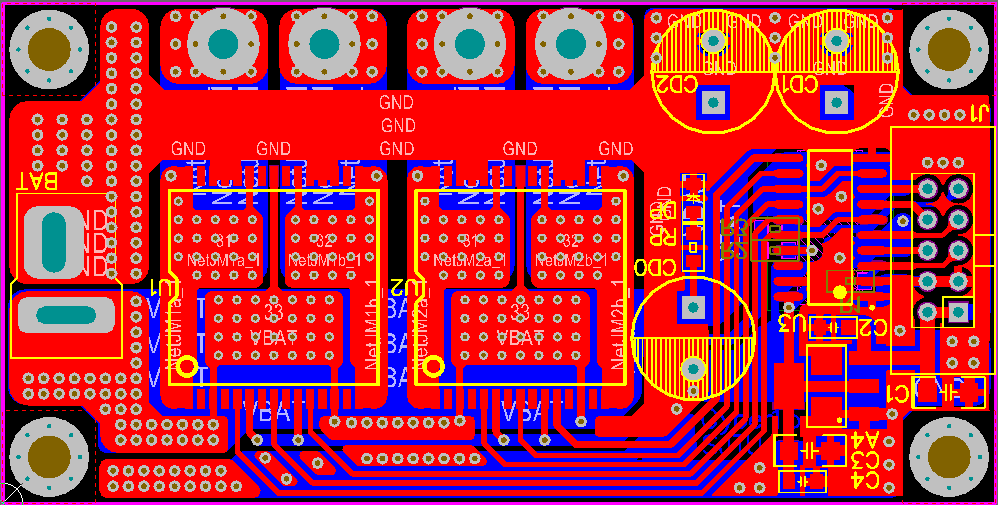
\includegraphics[width=0.35\textwidth]{chap3/DrvPCBTop.PNG}}
  \hspace{1in}
  \subfigure[PCB背面]{
    \label{fig:corepcb:b} %% label for second subfigure
    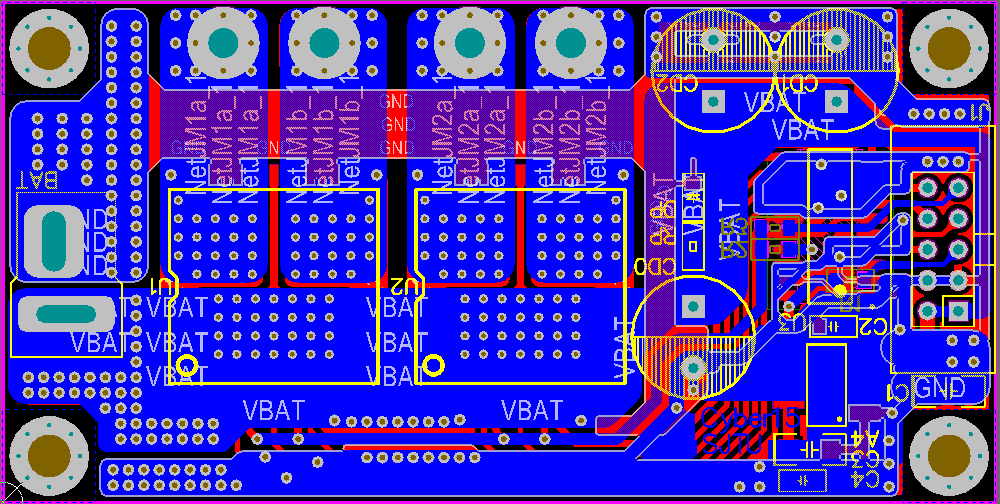
\includegraphics[width=0.35\textwidth]{chap3/DrvPCBBack.PNG}}
  \bicaption{驱动电路的设计PCB样图}{驱动电路的设计PCB样图}{Fig}{The PCB View of Driver Board}
\end{figure}

\subsection{编码器模块}
编码器模块实际上是比较简单的模块,其主要功能是为编码器提供片外计数器,并把结果反馈给主控板。在本设计中,选用的是CD4520芯片。这是一个最高计数值较小的高速用计数器。每个芯片的接线方法的电路原理图如图\upcite{ConSch}。\\
\begin{figure}[!htp]\label{fig.ConSch}
  \centering
  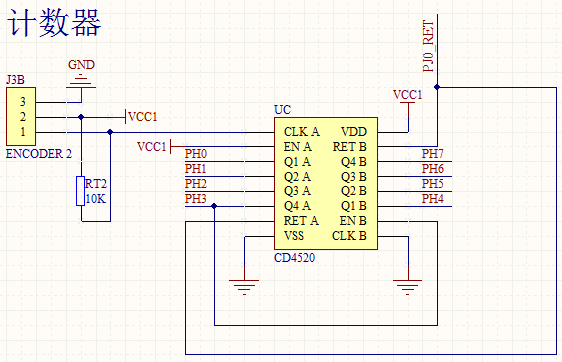
\includegraphics[width=0.8\textwidth]{chap3/counter.PNG}
  \bicaption{编码器用外部计数器接线图}{编码器用外部计数器接线图}{Fig}{Schematic of counters for encoder}
\end{figure}
\subsection{传感器模块}
传感器模块需要因传感器种类的不同而不同。在这里只对本设计需要用的超声波传感器的驱动电路进行讨论。因为传感器众多,为了节省片上资源,需要新的方法去驱动这么多传感器。其中一种方案就如笔者的设计,轮流激活传感器网络中的各个个体,这样可以复用同一套数据读取口,只需要不同的选通IO接口就可以了。这种方法充分的考虑到了片上资源不足的情况,极大的减少所要使用IO口的数量。传感器驱动网络的原理图如图\ref{fig.ultraSonic}所示。从图中可以看出PK7口是复用的,是有上升沿和下降沿检测中断的端口。如果使用译码器驱动选通的话,可以以供使用4个IO口驱动8个传感器。
\begin{figure}[!htp]\label{fig.ultraSonic}
  \centering
  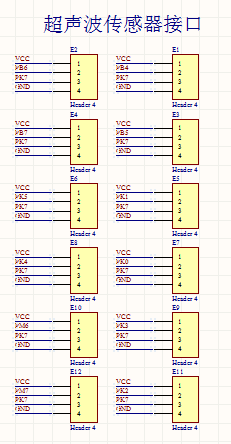
\includegraphics[width=0.4\textwidth]{chap3/ultraSonic.PNG}
  \bicaption{超声波传感器驱动板原理图}{超声波传感器驱动板原理图}{Fig}{Schematic of Ultrasonics Driver Unit}
\end{figure}


在本设计中选用的传感器是比较常见的HC-SR04模块。其有效检测距离是4cm到8m。超声波传感器不同于红外传感器,抗光线和环境干扰能力比较强,相对可靠。同时因为模块的常见性,又使其非常廉价。这款模块的实物图如图\ref{fig.ultraSonicReal} 所示。 \\
\begin{figure}[!htp]\label{fig.ultraSonicReal}
  \centering
  \subfigure[正面]{
    \label{fig:corepcb:a} %% label for first subfigure
    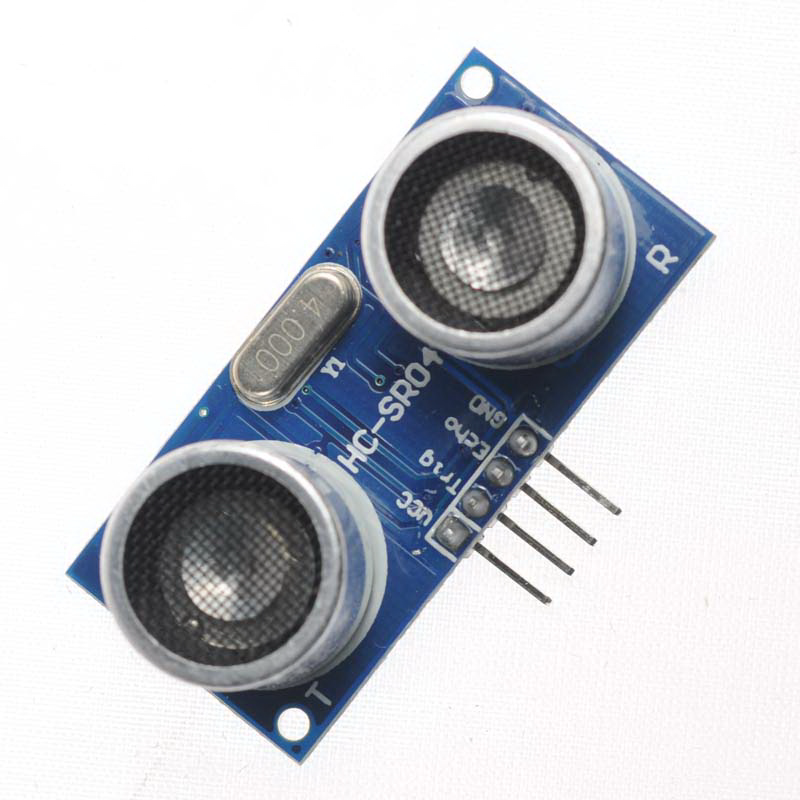
\includegraphics[width=0.35\textwidth]{chap3/HC_SR04.png}}
  \hspace{1in}
  \subfigure[背面]{
    \label{fig:corepcb:b} %% label for second subfigure
    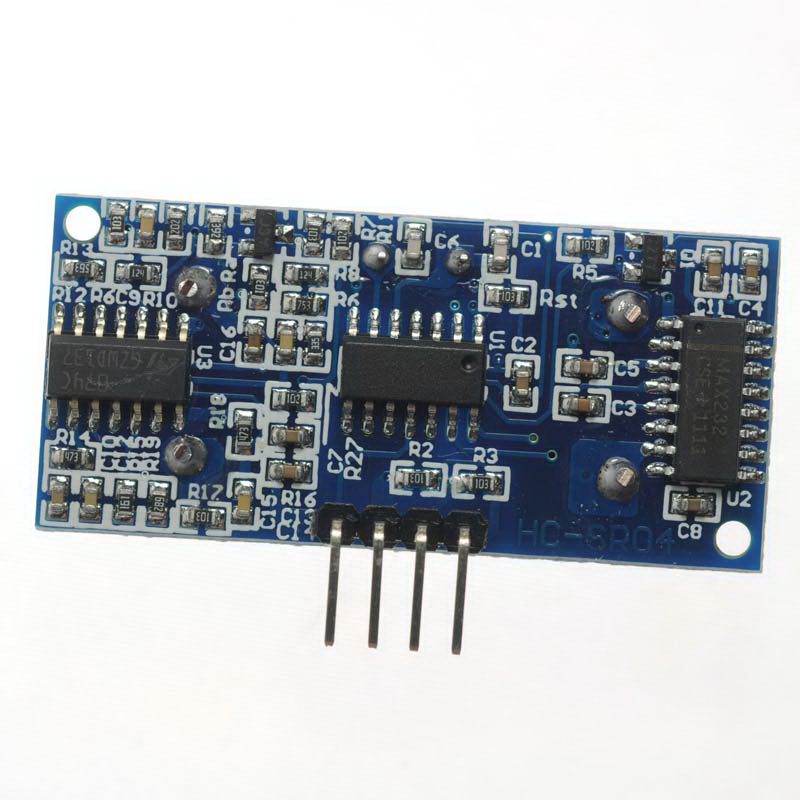
\includegraphics[width=0.35\textwidth]{chap3/HC_SR04back.png}}
  \bicaption{超声波传感器}{超声波传感器}{Fig}{Ultrasonics Sensor Unit}
\end{figure}
\subsection{模块间通讯接口}
\section{本章小结}


%%==================================================
%% chapter03.tex for SJTU Bachelor Thesis
%% version: 0.5.2
%% Encoding: UTF-8
%%==================================================

% \bibliographystyle{sjtu2} %[此处用于每章都生产参考文献]

\chapter{控制与智能避障算法}
\label{chap:algorithm}

在本章将主要介绍模块化移动机器人控制系统的软件系统。由于本移动机器人具有自主移动,自主定位,自动避障,地图生成和最优路径计算等功能,所以需要将其软件系统分为底盘电机驱动,车体定位,未知环境避障和探测地图绘制等部分。其中只有电机驱动部分是与选用的控制芯片有关系的,而其他诸部分皆是上层算法,所以处理驱动算法的程序不可移植外,其他部分皆可移植到其他系统中去。在下面的介绍中,除了会给出具体算法程序外,还会对每一部分算法的数学原理进行简单的介绍。

\section{底盘驱动算法}
底盘驱动采用了经典的H桥方案,通过单一IO口的高低电平来对方向进行控制,而在使能端接入PWM方波,通过控制占空比来控制电机的转速。控制占空比来控制转速的具体原理是,占空比的改变可以改变方波的等效电压。设一列方波的占空比是$a$,则在一个方波周期内等效电压与占空比的关系为 \\
\begin{equation}\label{eqn.equavalentVoltage}
V_{org}aT=V_{equ}T
\end{equation}
其中$V_{org}$是方波最大幅值,$T$为方波周期,$V_{equ}$为等效电压。通过公式\eqref{eqn.equavalentVoltage},可以得到\\
\begin{equation}
V_{equ} = aV_{org}
\end{equation}
等效电压与占空比呈简单线性关系。而通过电机的特性公式\eqref{eqn.motorCha} \\
\begin{equation}\label{eqn.motorCha}
V_{supply} = K_{e}\dot{\theta}
\end{equation}
可知电机转速和输入电压$V_{sipply}$成正比,这就意味轮子的转速与方波占空比成正比。所以控制轮子的转速只需要改变输入方波的占空比就可以了。但是占空比只给出了一个速度的相对关系,并没有与具体速度值的对应,所以控制的时候还要通过传感器的数据,对速度控制进行闭环。

电机系统所需输出口初始化,和一般电机控制程序如下。此段程序,是参考罗翔的程序所撰写。
\begin{lstlisting}[language={C}, caption={针对BTS7960的单片机初始化程序}]
#include "BTS7960B.h"
#include "SystemConfig.h"

/* Crystal's frequecy is 40MHz
   USE PPL change the bus frequecy*/
//---------宏参数定义-------------
#define HIGH   1
#define LOW    0
#define OUTPUT 1
#define INPUT  0

#define SETPWM23 0x0C                    //置1 PWM23选择项
#define CLRPWM23 (~SETPWM23)             //清零PWM23选择项
#define CLKB1D08 0x30                    //ClockB运行方式

#if SYS_BUS_FREQUENCY == SYSTEM_BUS_64M 
//64M-预分频: fA=2M, fB=4M(使用fB)    
    #define _PWMMAX 199                      //占空比最大值
    #define _PWMMIN 0                        //占空比最小值
    #define _PWMUNT 2    
#else                   
//其他分频: fA = 2.5MHz, fB = 5MHz,请在此基础上设定频率 
    #define _PWMMAX 249                      //占空比最大值
    #define _PWMMIN 0                        //占空比最小值 
    #define _PWMUNT 5/2   
#endif   

//---------操作函数定义-------------
void BTS7960BRestart(void)     
//重启函数:对需使用I/O口初始化
{
    DDRM_DDRM5 = OUTPUT;
    _BTSDRVE   = LOW   ;
    DDRM_DDRM4 = INPUT ;
    _BTSDRVS   = LOW   ;//Initial BITS OF PTM PORT 
    
    PWME     &= CLRPWM23;//关PWM23 
    
    //PWMPRCLK |= CLKB1D08;//ClockB frequency = 40MHz/8=5MHz
    //PWMSCLB   = 5       ;
    
    PWMPER2   = _PWMMAX ;//PWM2 frequency = 10kHz
    PWMDTY2   = _PWMMAX ;//占空比0 
    PWMPER3   = _PWMMAX ;//PWM3 frequency = 10kHz
    PWMDTY3   = _PWMMAX ;//占空比0    
    
    PWME     |= SETPWM23;
    
    BTS7960BEnable(HIGH) ;   
}

unsigned char BTS7960BControl(unsigned char ForwardPWM, unsigned char BackwardPWM)
//控制函数:正反转控制。输入PWM占空比,输出正反转状态 (输入均为百分之)
{
    unsigned char PStatus = BTS7960STOP;
    //PWM状态赋值
    PStatus = (ForwardPWM  > BackwardPWM)?BTS7960FORWARD:BTS7960BACKWARD;//电机运行状态判断
    PStatus = (ForwardPWM == BackwardPWM)?BTS7960STOP   :PStatus        ;
    
    ForwardPWM  = (ForwardPWM  > 100)?100:ForwardPWM ;
    BackwardPWM = (BackwardPWM > 100)?100:BackwardPWM;
    PWMDTY2 = (byte)((_PWMMAX < ForwardPWM  * _PWMUNT)?_PWMMIN:(_PWMMAX - ForwardPWM *_PWMUNT));//计算PWM占空比
    PWMDTY3 = (byte)((_PWMMAX < BackwardPWM * _PWMUNT)?_PWMMIN:(_PWMMAX - BackwardPWM*_PWMUNT));
    return PStatus;
}              
\end{lstlisting}
在底盘模块正常情况下是沿着算法所确定的方向匀速行进,速度只需规定一个为常数的占空比值就可以了。但是因为电机特性不一致的原因,即便规定同一PWM值,车体行进方向仍然可能偏离既定方向,所以要使底盘保持行进方向,就要对其行进角度进行闭环。这一功能的可以通过电子罗盘返回的数据来设计实现。这里将采用传统的PID算法来进行闭环程序的设计。PID系统的传递方程的拉普拉斯形式可以写为 \\
\begin{equation}
G(s)= K_p+\frac{K_i}{s}+K_ds
\end{equation}
其中$K_p$,$K_i$和$K_d$为PID方法的参数,对于系统方程,输入量是实际角度与计算角度的差值,输出量是驱动左轮与驱动右轮PWM占空比的差值。因为系统实际是离散的,所以需要将系统方程从S域映射到离散系统的Z域,关于这个控制器的C程序就是根据这一思想设计的,其伪代码可以表示如下。
\begin{lstlisting}[language={C}, caption={PID控制器伪代码}]
double KP = 一个合理的值;
double KI = 一个合理的值;
double KD = 一个合理的值;
double Error = 0;			//实际角度与计算角度的偏差
static double ErrorHis = 0;	//对于角度偏差的记录
static double ErrorAcu = 0;	//偏差积分

Error = AngleActual - AngleCalculated;
ErrorAcu += Error ;
DutyCycleDiff = KP*Error + KD*(Error-ErrorHis) + Ki*ErrorAcu ;
ErrorHis = Error;
\end{lstlisting}
关于底盘模块行进方向角度的计算将在未知环境避障算法部分介绍,关于遇到避障时转向的控制也将在那部分章节介绍。
\section{车体定位方案}
车体定位方案将直接决定了底盘模块的行进轨迹,对于是否完成目标的判断和地图的绘制等功能的实现。为了获得机器人准确的位置,在本设计中,使底盘集成了多种传感器模块。这其中包括轮式编码器,俗称拖地轮;IMU模块等单元,如果需要,则可以通过串口扩展,很容易的链接GPS模块。在下文中将详细介绍各个方案定位的数学原理,及坐标值获得的方法。

\subsection{拖地轮及方位角传感器定位}
拖地轮的机械结构设计已经在第二章的相应部分进行详细的叙述,在本节,将主要介绍基于拖地轮的定位算法。拖地轮的设计目标之一就要简化计算,所以将拖地轮固定在底盘模块相邻的两条边中央的位子上。底盘模块的坐标系,与轮子的位置如图\ref{fig.ChesisCoor} 所示。
\begin{figure}[!htp]
  \centering
  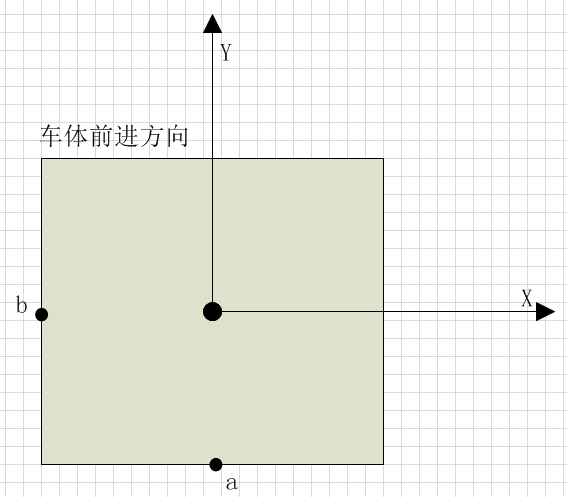
\includegraphics[width=0.5\textwidth]{chap4/ModelCordinates.PNG}
  \bicaption[fig.ChesisCoor]{底盘上坐标系的定义}{底盘上坐标系的定义}{Fig}{The Definition of the Coordinates On the Chassis}
\end{figure}

其中拖地轮a只能采集到与底盘模块y坐标轴平行的转动,同理拖地轮b只能采集到与底盘模块x坐标轴平行的转动。底盘的控制芯片将会以一定的周期进行对传感器信息的采集和对底盘模块体的控制。这一周期在本设计中为10毫秒,所以控制周期是100HZ。当每一个周期结束后,如果只有y方向的轮子采集到数据,则机器人体的世界坐标改变量为 \\
\begin{equation}
		\left\{
             \begin{array}{lcl}
            	\Delta x_{world} &= \Delta y\cdot \sin\theta \\
             	\Delta y_{world} &= \Delta y\cdot \cos\theta  
             \end{array}  
        \right.
\end{equation}
其中$x_{world}$,$y_{world}$为机器人体在世界坐标系中的坐标,$\theta$为机器人前进方向与世界坐标y轴所成的夹角。

同理当只有x方向的轮子采集到位移数据时,则机器人的世界坐标为 \\
\begin{equation}
		\left\{
             \begin{array}{lcl}
            	\Delta x_{world} &= \Delta x\cdot \cos\theta \\
             	\Delta y_{world} &= \Delta x\cdot \sin\theta  
             \end{array}  
        \right.
\end{equation}
而在同时采集到x与y方向的位移信息时,就需要用到一定的数学技巧来获得世界坐标的位移改变量。如图\ref{fig.ChesisMotion}所示,因为控制周期比较短,可以用直角模型来计算机器人体的位移,并假设车体的运动方向是初始时的运动方向保持不变,这样就可以通过机器人前进方向与世界坐标y轴的夹角和采集到的传感器信息来计算车体的实际位移了。
\begin{figure}[!htp]
  \centering
  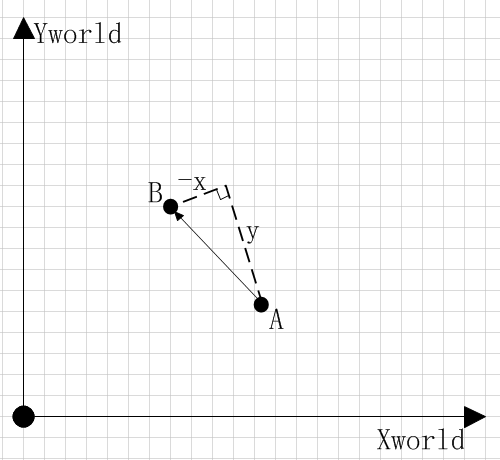
\includegraphics[width=0.5\textwidth]{chap4/OnMotion.PNG}
  \bicaption[fig.ChesisMotion]{机器人运动示意}{机器人运动示意}{Fig}{The Motion of the Robot in World Coordinates}
\end{figure}

这时世界坐标该变量的计算公式为 \\
\begin{equation}
		\left\{
             \begin{array}{lcl}
            	\Delta x_{world} &= \Delta y\cdot \sin\theta - \Delta x\cdot \cos\theta \\
             	\Delta y_{world} &= \Delta y\cdot \cos\theta + \Delta x\cdot \sin\theta  
             \end{array}  
        \right.
\end{equation}
\subsection{IMU定位}
通过IMU上所拥有的传感器元件可知,其对于位置的确定是依赖于积分的。加速度传感器的输出量是加速度,陀螺仪的输出量是角加速度,电子罗盘的输出量是角度。表征速度,位移和加速度关系的公式是 \\
\begin{equation}
D = \int\dot{D}=\int_T\int_T\ddot{D}
\end{equation}
所以只要对加速度进行二次积分就可以算出在某一轴上的位移分量。因为控制周期比较短,所以可以认为在一个周期$T$内,机器人是在做匀加速度,匀速度运动。如果以$\ddot{x}$和$\ddot{y}$作为在底盘模块参考系中的加速度传感器所能测出的加速度量,则坐标的数学表达式可以写作 \\
\begin{equation}
		\left\{
             \begin{array}{lcl}
            	\Delta x_{world} &= \ddot{y}\cdot T^2\cdot \sin\theta - \ddot{x}\cdot T^2\cdot \cos\theta \\
             	\Delta y_{world} &= \ddot{y}\cdot T^2\cdot \cos\theta + \ddot{x}\cdot T^2\cdot \sin\theta  
             \end{array}  
        \right.
\end{equation}
但是因为加速度传感器的噪声带会对积分误差的收敛造成影响,所以光靠加速度传感器的值做计算是不够的。还需要加上陀螺仪的输出值作参考。加速度值与陀螺仪测得的关于垂直于地面平面的转轴的角加速度值的关系是 \\
\begin{equation}
\arctan(\frac{\ddot{x}\cdot T^2}{\ddot{y}\cdot T^2}) = \int_T\int_T \ddot{\phi}
\end{equation}
其中$\phi$是角加速度。

但是仅仅是使用这个比较依然是不可靠的,还要对采集到的数据进行滤波。本设计根据Houtekamer等人\upcite{houtekamer1998data} 的文章,设计了对信号处理的卡尔曼滤波器。其C程序实现如下。
\begin{lstlisting}[language={C}, caption={Kalman滤波的C程序代码}]
float angle, angle_dot; 		//外部需要引用的变量
float Q_angle = 0.05, Q_gyro = 0.01, R_angle = 5, dt = 0.005;     
float P[2][2] = {{ 1, 0 },{ 0, 1 }} ;	
float Pdot[4] ={0,0,0,0} ;
const char C_0 = 1;
float q_bias, angle_err, PCt_0, PCt_1, E, K_0, K_1, t_0, t_1;
//-------------------------------------------------------
void Kalman_Filter(float angle_m,float gyro_m)			
{
	angle+=(gyro_m-q_bias) * dt;			//先验估计
	
	Pdot[0]=Q_angle - P[0][1] - P[1][0];	//先验估计误差协方差的微分
	Pdot[1]=- P[1][1];
	Pdot[2]=- P[1][1];
	Pdot[3]=Q_gyro;
	
	P[0][0] += Pdot[0] * dt;				// 先验估计误差协方差
	P[0][1] += Pdot[1] * dt;
	P[1][0] += Pdot[2] * dt;
	P[1][1] += Pdot[3] * dt;
	
	
	angle_err = angle_m - angle;			
	
	PCt_0 = C_0 * P[0][0];
	PCt_1 = C_0 * P[1][0];
	
	E = R_angle + C_0 * PCt_0;
	
	K_0 = PCt_0 / E;//Kk
	K_1 = PCt_1 / E;
	
	t_0 = PCt_0;
	t_1 = C_0 * P[0][1];

	P[0][0] -= K_0 * t_0;					//后验估计误差协方差
	P[0][1] -= K_0 * t_1;
	P[1][0] -= K_1 * t_0;
	P[1][1] -= K_1 * t_1;
	
	angle	+= K_0 * angle_err;				//后验估计
	q_bias	+= K_1 * angle_err;				//后验估计
	angle_dot = gyro_m-q_bias;				//输出值(后验估计)的微分 = 角速度
}
\end{lstlisting}
\section{未知环境避障算法}
在本设计中采用了虚拟势能场的算法来实现路径计算和自动避障的。这一算法最先由Khatib \upcite{khatib1986real}提出,并应用于机械臂行进路线的规划。后来虚拟势场的概念经由Yoram Koren等人\upcite{koren1991potential} 的发展,而可以应用到平面移动物体的二维运动规划中。

基本的虚拟势场思想主要是引入了两个虚拟力。一个为虚拟引力,一个为虚拟斥力。虚拟引力是指运动体与目标点之间的力,虚拟斥力是指运动体与障碍物之间的力。目标点在全局坐标系中的位置是已知的,所以在初始状态下就存在着引力场的作用,是机器人向目标点运动。因为势能的等势线为圆形,所以只有运动物体向着目标点前进,才是势能变化梯度最大方向。因此在某种意义上讲,由虚拟引力所计算出的运动方向是最优的。在本设计中,设计的机器人所处的环境是未知的,就是说初始条件下并无障碍物的存在,而在运动过程中会遇到障碍物,并在障碍物的斥力影响下而改变运动方向。这说明斥力是一种短程力,它的作用范围是有限的。

在本设计中接纳了耿兆丰等人\upcite{gzf1992VPpath} 的方案,将目标点产生的势场$P$定义为 \\
\begin{equation}
P = r^2/2 = [(x-x_t)^2+(y-y_t)^2]/2
\end{equation}
其中$x_t$,$y_t$为目标点坐标。则此时机器人所处位置的势场梯度可以表示为 \\
\begin{equation}
\nabla P = \frac{\partial P}{\partial x}i+\frac{\partial P}{\partial y}j = (x-x_t)i+(y-y_t)
\end{equation}
因此引力可以表示为 \\
\begin{equation}
F_{att} = K(|\nabla P|_{r=d})=Kd
\end{equation}
其中$K$为引力常数。

对于斥力,正如上文所说,为短程力,所以其应该具有随着距离的变长而减弱的特点,如果斥力能与距离成反比的话,将符合这一要求。所以斥力的形式应为 \\
\begin{equation}
F_{rep} = \frac{K_r}{(x-x_o)^2+(y-y_o)^2}
\end{equation}
其中$K_r$为斥力常数。与引力不同,斥力是一个三维力,计算斥力时不仅相对于质心坐标,而是相对于传感器所在的点,所以$x_0$和$y_0$是每个传感器点的坐标。在此处分母使用距离的平方是因为,第一可以简化计算,提高计算速度;第二可以加快斥力的衰减和增加。斥力的作用方向即为力场梯度方向。 \\
\begin{equation}
\nabla F_{rep} = -2\frac{K_r(x-x_o)}{((x-x_o)^2+(y-y_o)^2)^2}i-2\frac{K_r(y-y_o)}{((x-x_o)^2+(y-y_o)^2)^2}j
\end{equation}
其方向矢量可以化简的表示为$[-(x-x_o)\; -(y-y_o)]$ 。因为斥力是个短程力,所以要设定一个阀值,使斥力小于这一阀值时为0。

在有了引力与斥力的公式后,就可以对每个点对车体的作用积分而算出合力,再通过合力的方向来计算机器人的行动方向。本机器人的控制系统所有的方向都表示为机器人前进方向与世界坐标系的y轴的夹角。算法的示意图如图\ref{fig.pathPlaning1}所示。
\begin{figure}[!htp]
  \centering
  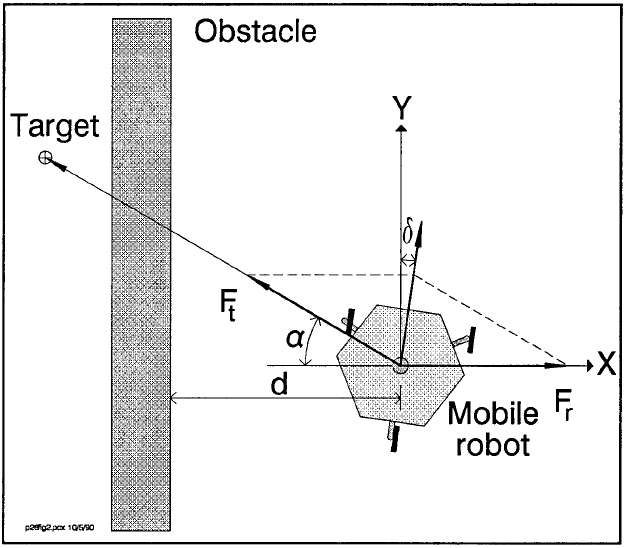
\includegraphics[width=0.5\textwidth]{chap4/pathPlaning1.PNG}
  \bicaption[fig.pathPlaning1]{虚拟势能蔽障算法示意图}{虚拟势能蔽障算法示意图\upcite{koren1991potential}}{Fig}{Motion of a mobile robot applying a potential field algorithm}
\end{figure}

但是这种算法存在的问题就是,如果障碍物足够大,可能存在着受力平衡点,使机器人永远无法越过障碍物。为了改变这一现象,不得不对机器人引入惯性。但是光引入惯性还是不够的,同时还要引入运动方向锁,来使最后的搜索过程可以得到收敛解。
\section{地图生成和最优路径生成}
关于地图的绘制,是受到了David Waller等人\upcite{waller1998transfer}研究的启发,同时参考了周斌等人\upcite{zb2006memory}的研究。底盘模块进行这样设计的原因是如果需要多次重复的使机器人从某一出发点到达某一目标点,在经过第一次机器人的探索后,可以记住环境信息,并在下次进行相同任务时,可以直接沿着最优路径前进而不需要重新探测。则可以大大加快机器人在同一环境长时间重复执行同一任务时的效率。

与周斌给出的方法不同,在本设计中,地图信息并不是保存在车体的控制器里,而是底盘模块会将数据发回给上位机,并由上位机处理并绘制地图,再通过上位机来计算最优路径,返回给片上系统。地图绘制的过程主要还是靠传感器模块标出障碍物的坐标,并根据这一坐标和机器人本身坐标尺寸来绘制障碍物和机器人可通过通道。

而最优路径生成这是通过现将绘制的地图网格化,然后从目标点出发向起始点回溯的去评价每一个点。评价公式就是与目标点的距离。在评价过程中只关心处在网格节点上的点,只要网格足够小,最后所得到的结果是可信的。当所有点评价完毕后,出发点会有多种评价值。找出最小的评价值,就可以找出最优的路径。然后连接这条线路上的每一个点,对这条路径的关键点信息进行计算并返回给底盘模块进行存储。这样就完成了最优路径生成的过程。

\section{本章小结}
本章主要介绍了所设计的移动模块化机器人系统的软件部分。这部分内容主要是针对轮式底盘和超声波传感器部分所设计的。本章节只涉及到了本移动式模块化平台的关键算法。关键算法包括4部分,第一为底盘的驱动算法,这是其他对车体控制算法的基础;其次是车体定位算法,这些算法是决定蔽障是否可行的关键;接下来是避障算法,详细介绍了机器人是如何能绕过障碍物而自主向目标点行进的;最后是地图的绘制和最优路径的生成,其中地图绘制是最优路径生成的基础。

%\include{body/chapter01}
%%%==================================================
%% chapter02.tex for SJTU Bachelor Thesis
%% version: 0.5.2
%% Encoding: UTF-8
%%==================================================

\chapter{一些 \LaTeX 排版的例子}
\label{chap:example}

\section{数学排版的例子}
\label{sec:matheq}

\subsection{公式排版}
\label{sec:eqformat}

这里有举一个长公式排版的例子,来自\href{http://www.tex.ac.uk/tex-archive/info/math/voss/mathmode/Mathmode.pdf}{《Math mode》}:

\begin {multline}
  \frac {1}{2}\Delta (f_{ij}f^{ij})=
  2\left (\sum _{i<j}\chi _{ij}(\sigma _{i}-
    \sigma _{j}) ^{2}+ f^{ij}\nabla _{j}\nabla _{i}(\Delta f)+\right .\\
  \left .+\nabla _{k}f_{ij}\nabla ^{k}f^{ij}+
    f^{ij}f^{k}\left [2\nabla _{i}R_{jk}-
      \nabla _{k}R_{ij}\right ]\vphantom {\sum _{i<j}}\right )
\end{multline}

\subsubsection{一个四级标题}
\label{sec:depth4}

这是全文唯一的一个四级标题。在这部分中将演示可伸长符号(箭头、等号的例子)的例子,以及如何在可伸长的符号上标注。在\href{http://zhou63.ahut.edu.cn/latex/ctexfaq.pdf}{《CTeX常见问题集》}中也由类似的介绍。
首先需要在diss.tex导言区引入如下的内容:

\begin{lstlisting}[language={TeX}, caption={插入导言区的内容}]
  \makeatletter
  \def\ExtendSymbol#1#2#3#4#5{\ext@arrow 0099{\arrowfill@#1#2#3}{#4}{#5}}
  \def\RightExtendSymbol#1#2#3#4#5{\ext@arrow 0359{\arrowfill@#1#2#3}{#4}{#5}}
  \def\LeftExtendSymbol#1#2#3#4#5{\ext@arrow 6095{\arrowfill@#1#2#3}{#4}{#5}}
  \makeatother
  
  \newcommand\myRightarrow[2][]{\RightExtendSymbol{=}{=}{\Rightarrow}{#1}{#2}}
  \newcommand\myLeftarrow[2][]{\LeftExtendSymbol{\Leftarrow}{=}{=}{#1}{#2}}
  \newcommand\myBioarrow[2][]{\ExtendSymbol{\Leftarrow}{=}{\Rightarrow}{#1}{#2}}
  \newcommand\myLongEqual[2][]{\ExtendSymbol{=}{=}{=}{#1}{#2}}
\end{lstlisting}

然后,在正文插入如代码\ref{mathextend}所示的内容。效果如下:

\begin{lstlisting}[language={TeX}, caption={可伸长的符号},label=mathextend,float]
  \begin{eqnarray}
    f(x) & \myBioarrow{A=B}  & B \\
    & \myLongEqual{A=B} & B \\
    & \myLeftarrow[A=B^2]{B=A^2} & B \nonumber \\
    & \myRightarrow{B^2=A^2} & B
  \end{eqnarray}
\end{lstlisting}

\begin{displaymath}
    A \xleftarrow{n=0} B \xrightarrow[LongLongLongLong]{n>0} C 
\end{displaymath}

\begin{eqnarray}
  f(x) & \myBioarrow{A=B}  & B \\
  & \myLongEqual{A=B} & B \\
  & \myLeftarrow[A=B^2]{B=A^2} & B \nonumber \\
  & \myRightarrow{B^2=A^2} & B
\end{eqnarray}

又如:

\begin{align}
  \label{eq:none}
  & I(X_3;X_4)-I(X_3;X_4|X_1)-I(X_3;X_4|X_2) \nonumber \\
  \myLongEqual{a)}\, & [I(X_3;X_4)-I(X_3;X_4|X_1)]-I(X_3;X_4|\tilde{X}_2) \\
  \myLongEqual[\rule{0.28cm}{0cm}]{}\, & I(X_1;X_3;X_4)-I(X_3;X_4|\tilde{X}_2)
\end{align}


\subsection{定理环境}

模板中定义了丰富的定理环境
algo(算法),thm(定理),lem(引理),prop(命题),cor(推论),defn(定义),conj(猜想),exmp(例),rem(注),case(情形),
bthm(断言定理),blem(断言引理),bprop(断言命题),bcor(断言推论)。
amsmath还提供了一个proof(证明)的环境。
这里举一个``定理''和``证明''的例子。
\begin{thm}[留数定理]
\label{thm:res}
  假设$U$是复平面上的一个单连通开子集,$a_1,\ldots,a_n$是复平面上有限个点,$f$是定义在$U\backslash \{a_1,\ldots,a_n\}$上的全纯函数,
  如果$\gamma$是一条把$a_1,\ldots,a_n$包围起来的可求长曲线,但不经过任何一个$a_k$,并且其起点与终点重合,那么:

  \begin{equation}
    \label{eq:res}
    \ointop_{\gamma}f(z)\,\mathrm{d}z = 2\uppi\mathbf{i}\sum^n_{k=1}\mathrm{I}(\gamma,a_k)\mathrm{Res}(f,a_k)
  \end{equation}

  如果$\gamma$是若尔当曲线,那么$\mathrm{I}(\gamma, a_k)=1$,因此:

  \begin{equation}
    \label{eq:resthm}
    \ointop_{\gamma}f(z)\,\mathrm{d}z = 2\uppi\mathbf{i}\sum^n_{k=1}\mathrm{Res}(f,a_k)
  \end{equation}

      % \oint_\gamma f(z)\, dz = 2\pi i \sum_{k=1}^n \mathrm{Res}(f, a_k ). 

  在这里,$\mathrm{Res}(f, a_k)$表示$f$在点$a_k$的留数,$\mathrm{I}(\gamma,a_k)$表示$\gamma$关于点$a_k$的卷绕数。
  卷绕数是一个整数,它描述了曲线$\gamma$绕过点$a_k$的次数。如果$\gamma$依逆时针方向绕着$a_k$移动,卷绕数就是一个正数,
  如果$\gamma$根本不绕过$a_k$,卷绕数就是零。

  定理\ref{thm:res}的证明。
  
  \begin{proof}
    首先,由……

    其次,……

    所以……
  \end{proof}
\end{thm}

上面的公式例子中,有一些细节希望大家注意。微分号d应该使用``直立体'',也就是用mathrm包围起来。
并且,微分号和被积函数之间应该有一段小间隔,可以插入\verb+\,+得到。
斜体的$d$通常只作为一般变量。
i,j作为虚数单位时,也应该使用``直立体'',为了明显,还加上了粗体,例如\verb+\mathbf{i}+。斜体$i,j$通常用作表示``序号''。
其他字母在表示常量时,也推荐使用``直立体'',譬如,圆周率$\uppi$(需要upgreek宏包),自然对数的底$\mathrm{e}$。


\section{向文档中插入图像}
\label{sec:insertimage}

\subsection{支持的图片格式}
\label{sec:imageformat}

\XeTeX 可以很方便地插入PDF、EPS、PNG、JPG格式的图片。

插入PNG/JPG的例子如\ref{fig:SRR}所示。
这两个水平并列放置的图共享一个``图标题''(table caption),没有各自的小标题。

\begin{figure}[!htp]
  \centering
  
\includegraphics[width=0.3\textwidth]{chap2/testpng}
  \hspace{1cm}
  
\includegraphics[width=0.3\textwidth]{chap2/testjpg}
  \bicaption[fig:SRR]{这里将出现在插图索引中}{中文题图}{Fig}{English caption}
\end{figure}

这里还有插入eps图像和pdf图像的例子,如图\ref{fig:pdfeps}。这里将EPS和PDF图片作为子图插入,每个子图有自己的小标题。并列子图的功能是使用subfigure宏包提供的。

\begin{figure}
  \centering
  \subfigure[EPS Figure]{
    \label{fig:epspdf:a} %% label for first subfigure
    
\includegraphics[width=0.3\textwidth]{chap2/testeps}}
  \hspace{1in}
  \subfigure[PDF Figure]{
    \label{fig:epspdf:b} %% label for second subfigure
    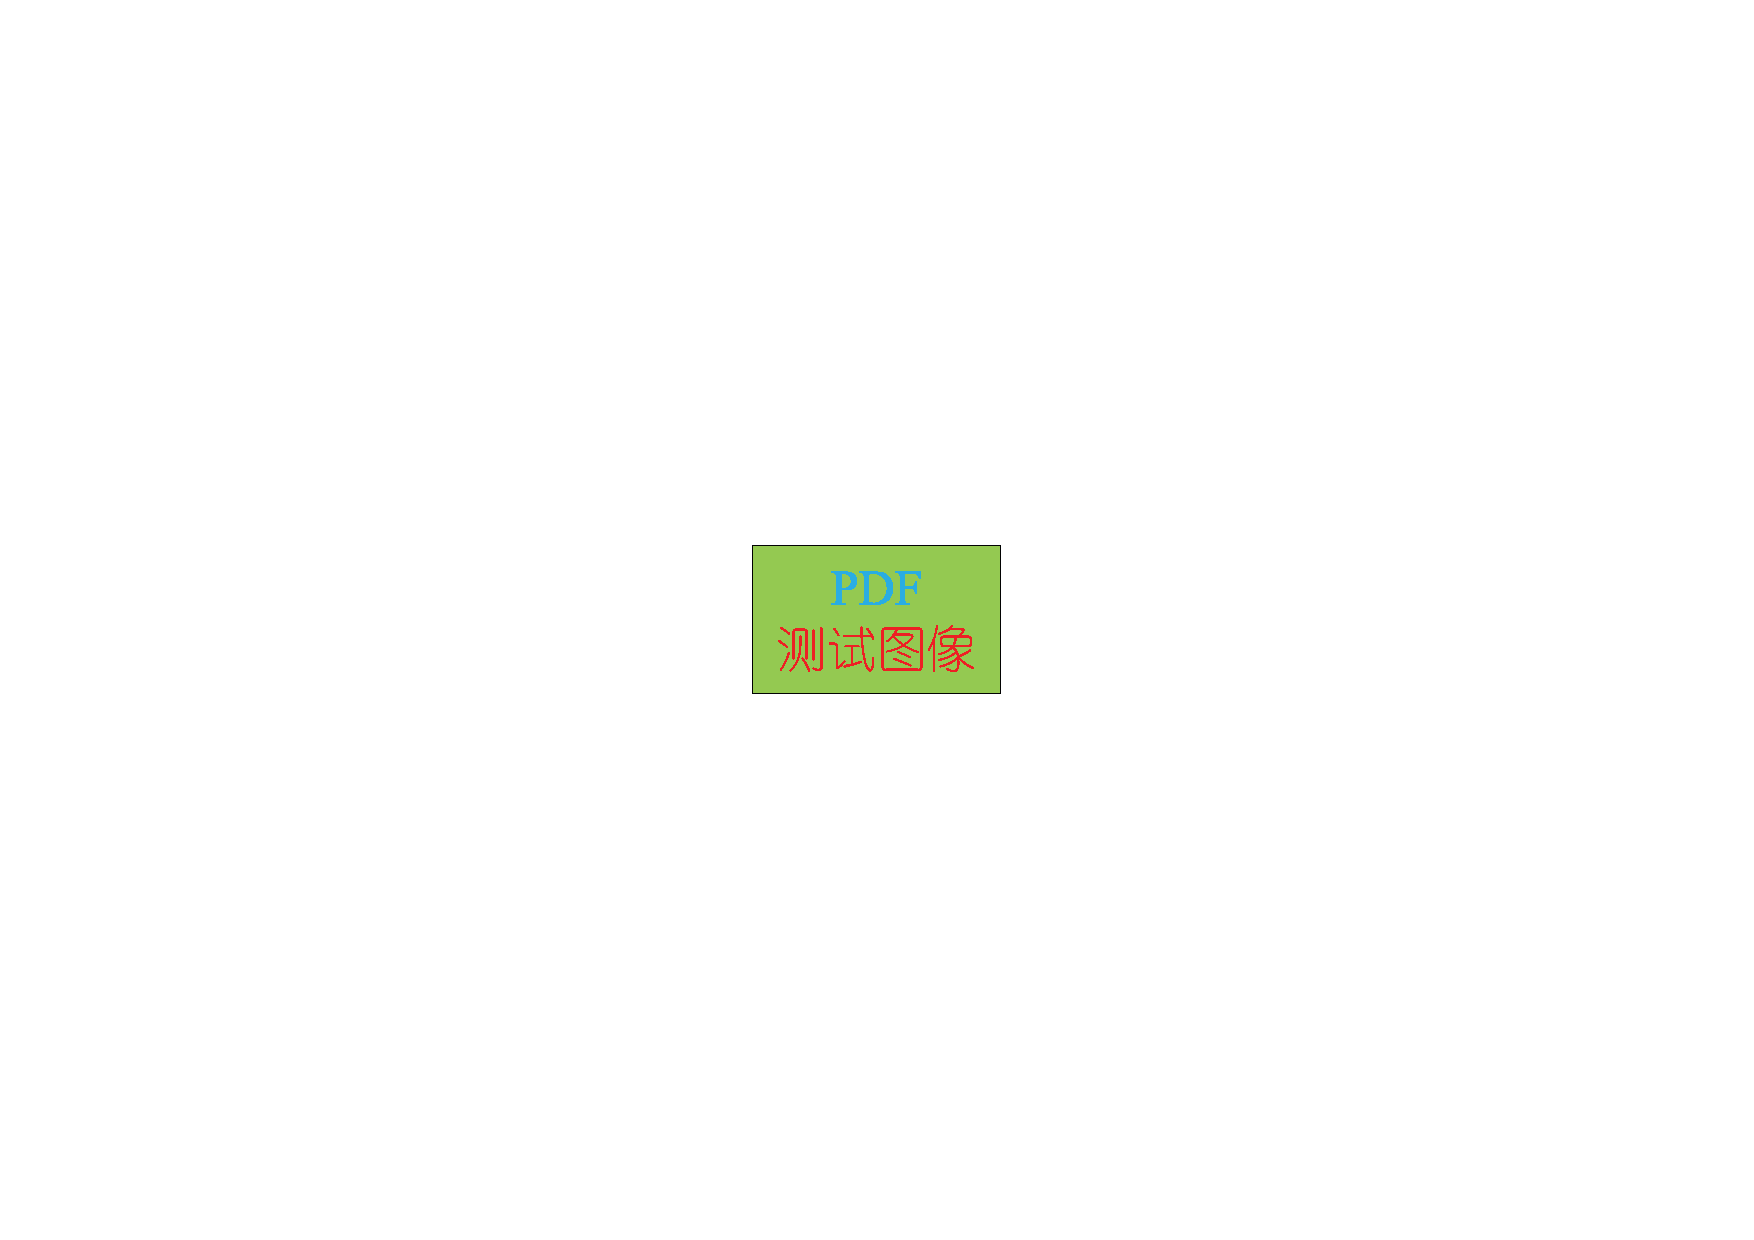
\includegraphics[angle=-90,origin=br,width=0.3\textwidth]{chap2/testpdf.pdf}}
  \bicaption[fig:pdfeps]{插入eps图像和pdf图像}{插入eps和pdf的例子}{Fig}{An EPS and PDF demo}
\end{figure}

更多关于 \LaTeX 插图的例子可以参考\href{http://www.cs.duke.edu/junhu/Graphics3.pdf}{《\LaTeX 插图指南》}。

\subsection{长标题的换行}
\label{sec:longcaption}

图\ref{fig:longcaptionbad}和图\ref{fig:longcaptiongood}都有比较长图标题,通过对比发现,图\ref{fig:longcaptiongood}的换行效果更好一些。
其中使用了minipage环境来限制整个浮动题的宽度。

\begin{figure}[!htp]
 \centering
 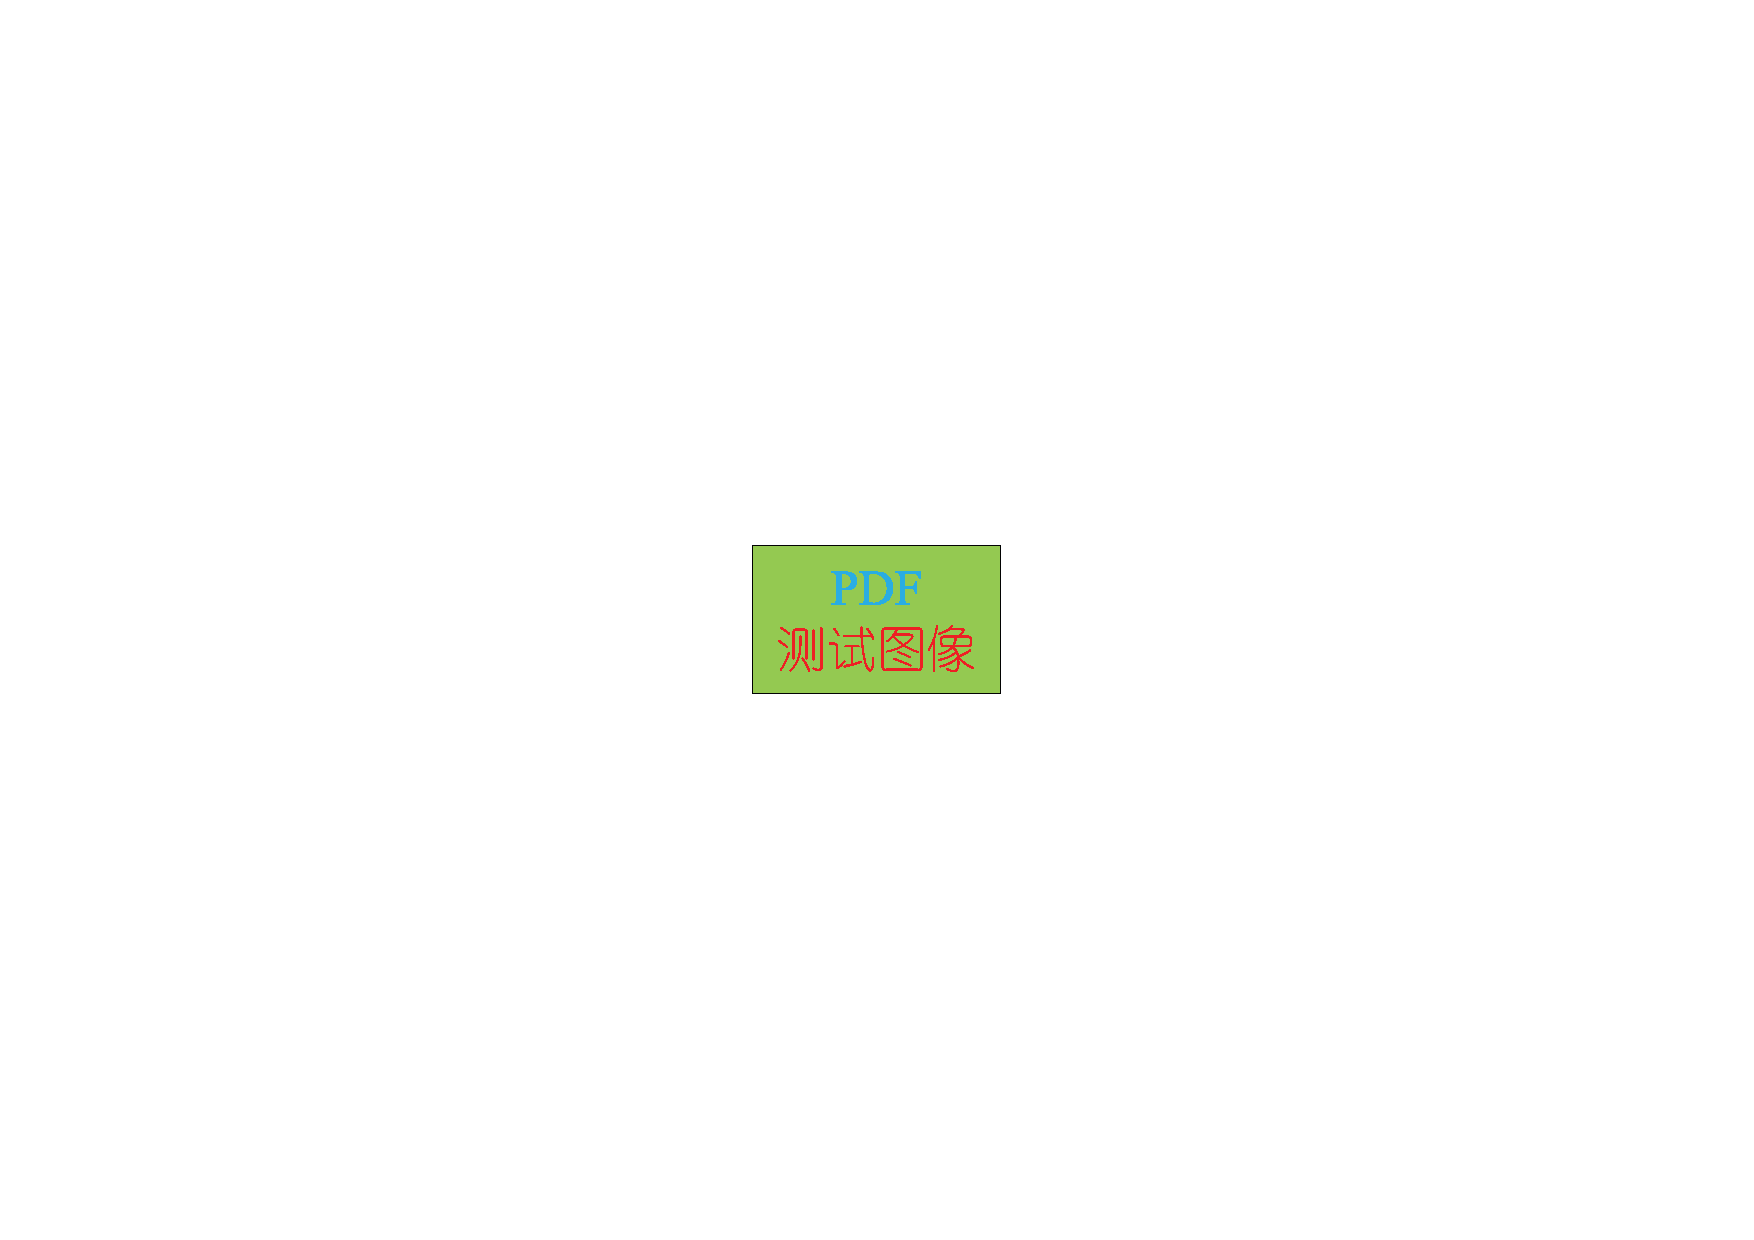
\includegraphics[angle=-90,origin=br,width=4cm]{chap2/testpdf.pdf}
 \bicaption[fig:longcaptionbad]{这里将出现在插图索引}{海交通大学是我国历史最悠久的高等学府之一,是教育部直属、教育部与上海市共建的全国重点大学.}{Fig}{Where there is a will, there is a way.}
\end{figure}


  \begin{figure}[!hbp]
    \centering
    \begin{minipage}[b]{0.6\textwidth}
      \captionstyle{\centering}
      \centering
      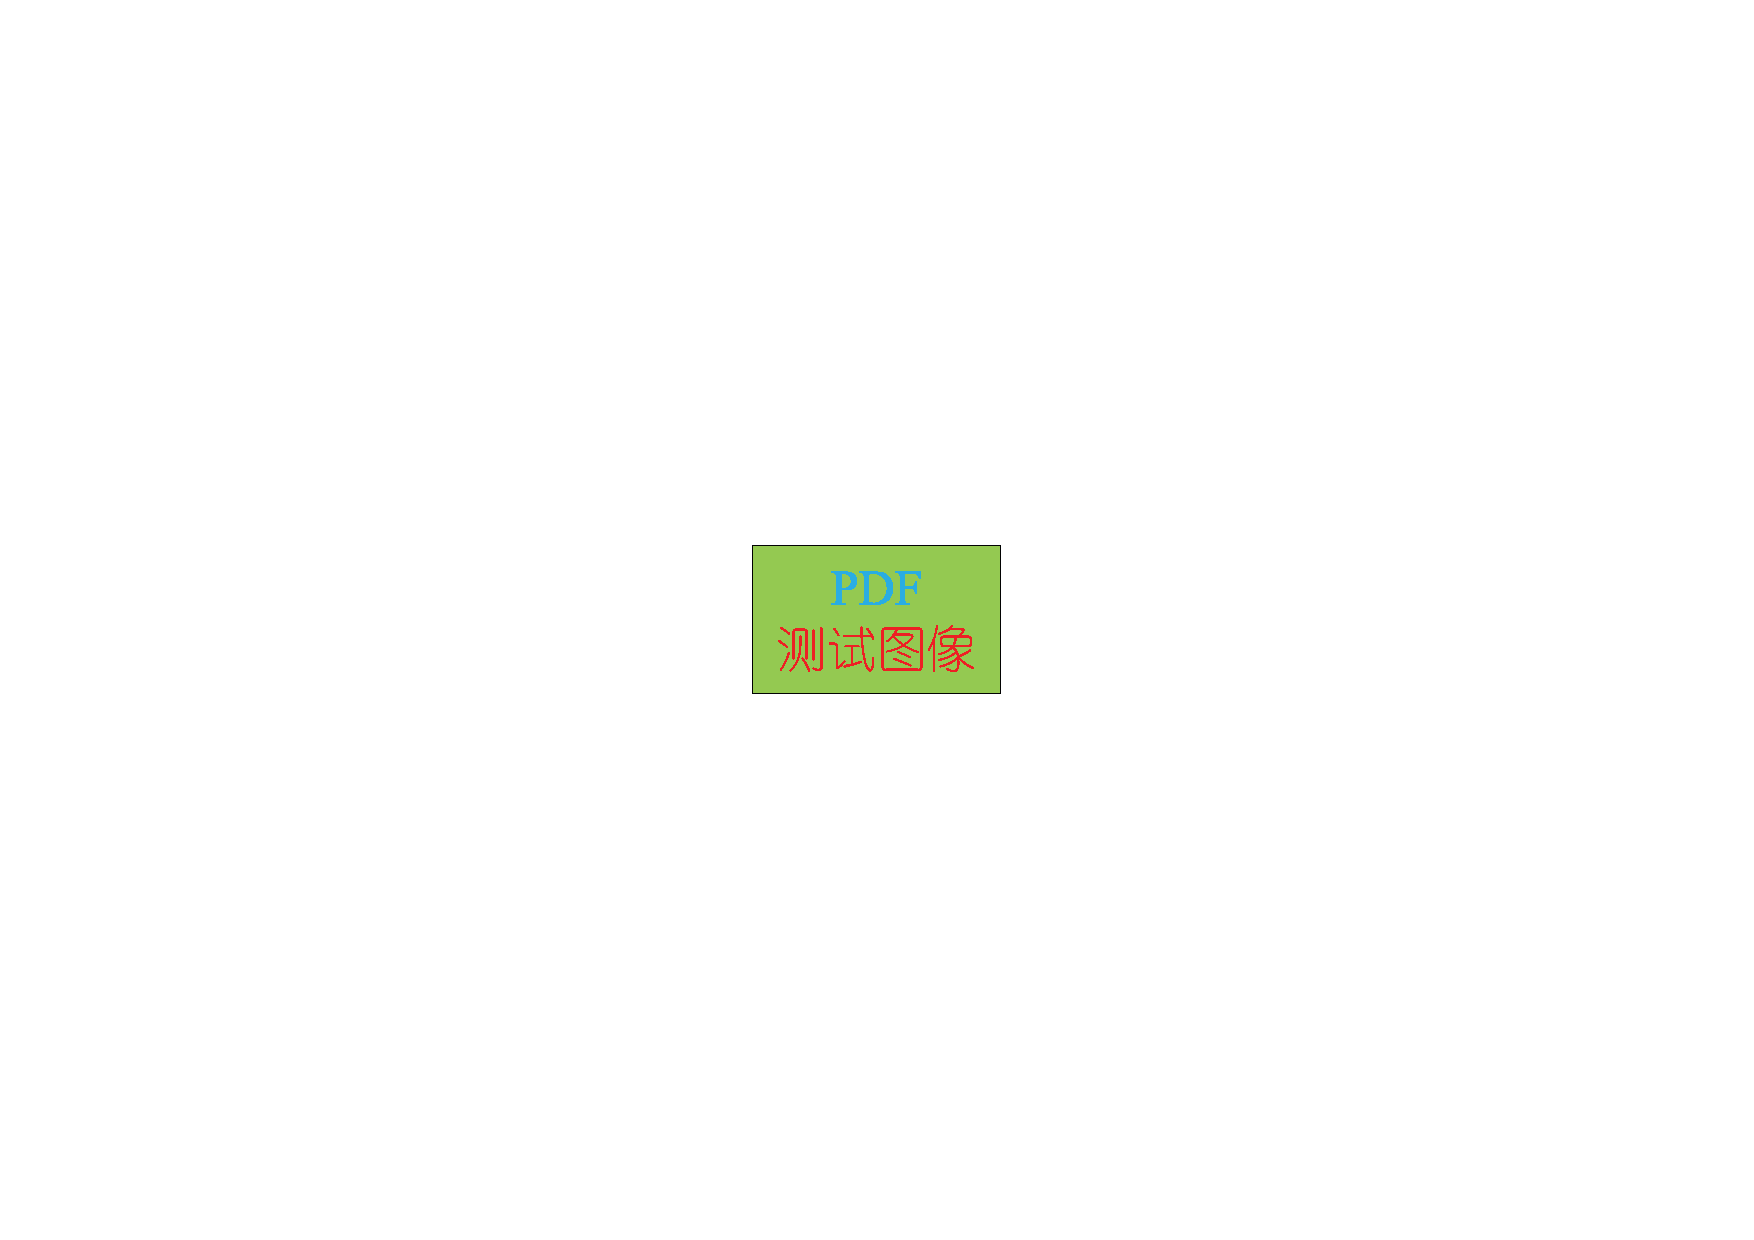
\includegraphics[angle=-90,origin=br,width=4cm]{chap2/testpdf.pdf}
      \bicaption[fig:longcaptiongood]{这里将出现在插图索引}{海交通大学是我国历史最悠久的高等学府之一,是教育部直属、教育部与上海市共建的全国重点大学.}{Fig}{Where there is a will, there is a way.}
    \end{minipage}     
  \end{figure}

  
\section{表格的例子}
\label{sec:tab}

这一节给出的是一些表格的例子,如表\ref{tab:firstone}所示。

\begin{table}[!hpb]
  \centering
  \bicaption[tab:firstone]{指向一个表格的表目录索引}{一个颇为标准的三线表格\footnotemark[1]}{Table}{A Table}
  \begin{tabular}{@{}llr@{}} \toprule
    \multicolumn{2}{c}{Item} \\ \cmidrule(r){1-2}
    Animal & Description & Price (\$)\\ \midrule
    Gnat & per gram & 13.65 \\
    & each & 0.01 \\
    Gnu & stuffed & 92.50 \\
    Emu & stuffed & 33.33 \\
    Armadillo & frozen & 8.99 \\ \bottomrule
  \end{tabular}
\end{table}
\footnotetext[1]{这个例子来自\href{http://www.ctan.org/tex-archive/macros/latex/contrib/booktabs/booktabs.pdf}{《Publication quality tables in LATEX》}(booktabs宏包的文档)。这也是一个在表格中使用脚注的例子,请留意与threeparttable实现的效果有何不同。}

下面一个是一个更复杂的表格,用threeparttable实现带有脚注的表格,如表\ref{tab:footnote}。

\begin{table}[!htpb]
  \bicaption[tab:footnote]{出现在表目录的标题}{一个带有脚注的表格的例子}{Table}{A Table with footnotes}
  \centering
  \begin{threeparttable}[b]
     \begin{tabular}{ccd{4}cccc}
      \toprule
      \multirow{2}{6mm}{total}&\multicolumn{2}{c}{20\tnote{1}} & \multicolumn{2}{c}{40} &  \multicolumn{2}{c}{60}\\
      \cmidrule(lr){2-3}\cmidrule(lr){4-5}\cmidrule(lr){6-7}
      &www & k & www & k & www & k \\
      \midrule
      &$\underset{(2.12)}{4.22}$ & 120.0140\tnote{2} & 333.15 & 0.0411 & 444.99 & 0.1387 \\
      &168.6123 & 10.86 & 255.37 & 0.0353 & 376.14 & 0.1058 \\
      &6.761    & 0.007 & 235.37 & 0.0267 & 348.66 & 0.1010 \\
      \bottomrule
    \end{tabular}
    \begin{tablenotes}
    \item [1] the first note.% or \item [a]
    \item [2] the second note.% or \item [b]
    \end{tablenotes}
  \end{threeparttable}
\end{table}

\section{参考文献管理}

参考文献的管理是这个学位论文模板又一个有趣的地方。

\subsection{将参考文献的内容与表现分离}

这个论文模板使用BibTeX处理参考文献,这又是一个``内容''与``表现形式''分离的极好例子
\footnote{当然,你也可以手动编参考文献item,直接插入文档中。}。
参考文献的``内容''就是reference文件夹下的chap\textit{xx}.bib,参考文献的元数据(名称、作者、出处等)以一定的格式保存在这些纯文本文件中。
.bib文件也可以理解为参考文献的``数据库'',正文中所有引用的参考文件条目都会从这些文件中``析出''。
控制参考文献条目``表现形式''(格式)的是.bst文件。.bst文件定义了参考文献风格,使用不同的参考文献风格能将同一个参考文献条目输出成不同的格式。
当然,一个文档只能使用一个参考文献风格。本模板使用的是国标GBT7714风格的参考文献。

BibTeX的工作过程是这样的:
BibTeX读取.aux(第一次运行latex得到的)看看你引用了什么参考文献条目,
然后到.bib中找相关条目的信息,
最后根据.bst的格式要求将参考文献条目格式化输出,写到.bbl文件中。
在运行latex将.bbl插入文档之前,你可以用文本编辑器打开它,做一些小的修改。
你会发现,.bbl的格式和你自己手动写item很相似,它已经被赋予了一定的``表现形式''。

.bib数据库中的参考文献条目可以手动编写,也可以在google的学术搜索中找到。
各大数据库\footnote{譬如SCOPUS, IEEE, OSA等。}也支持将参考文献信息导出为.bib,省时省力。
以Google学术搜索为例:进入\url{http://scholar.google.com},在``学术搜索设置''中,将``文献管理软件''设为``显示导入BibTeX''的连接,保存退出。
然后学术搜索找到文献下会有``导出到BibTeX''连接,点击后Firefox会打开新的标签页,出现类似代码\ref{googlescholar}所示的内容
\footnote{展示这些.bib条目使用了listings宏包,因为listings宏包协调中文的能力很糟糕,所以读者在查看模板的这部分源代码时会看到一些非常麻烦的东西。并且,直接将源代码的这部分内容复制到.bib中可能还会出错。我的建议是:这部分内容留意PDF就足够了。}。
请注意,这个条目离``规范''还有一些距离。

  \begin{lstlisting}[caption={从Google Scholar找到的,但并不规范的.bib条目}, label=googlescholar, float, escapeinside="", numbers=none]
    @phdthesis{"白2008信用风险传染模型和信用衍生品的定价",
      title={{"信用风险传染模型和信用衍生品的定价"}},
      author={"白云芬"},
      year={2008},
      school={"上海交通大学"}
    } 
  \end{lstlisting}

  上面的.bib条目的``名字''\cndash{}``白2008信用风险传染模型和信用衍生品的定价'',包含ASCII以外的字符,BibTeX无法处理;
  条目还缺少了address域,这样编译出来的结果会出现``地址不详'';
  并且,条目还缺少language域,BibTeX需要language域来判断是否是中文参考文献。
  将上面的条目修正(改英文名、增加address和language域),复制到本地的.bib文件中就可以了。
  显然,这里描述的是参考文献的内容,而不是表现形式。

  \begin{lstlisting}[caption={一个符合规范的.bib条目}, label=itemok, float, escapeinside="", numbers=none]
    @phdthesis{bai2008,
      title={{"信用风险传染模型和信用衍生品的定价"}},
      author={"白云芬"},
      year={2008},
      language={zh},
      address={"上海"},
      school={"上海交通大学"}
    } 
  \end{lstlisting}

由于中英文参考文献处理起来有差异,所以需要在参考文献中标注是否是中文文献。
确切地说,BibTeX并不具有区分中英文参考文献的``智能'',这种智慧的来源是.bst文——它定义了处理参考文献的规则。
GBT7714-2005NLang.bst中规定:.bib中的条目,如果条目的``language''域非空,就被认为是中文文献,否则被认为是英文文献。
例如,刚才的文献,就会被认为是中文参考文献,采取一些针对中文的处理方式。

最后,这个条目被bibtex处理后,赋予了一定的``表现形式'',在.bbl文件中以下面的样子出现。
你还可以对它进行小的修改。
再次运行latex之后,它将被插入到文档中。

\begin{lstlisting}[caption={.bbl中被格式化之后的条目}, escapeinside="", numbers=none]
\bibitem["白云芬(2008)"]{bai2008}
  \textsc{"白云芬"}.
  \newblock {"信用风险传染模型和信用衍生品的定价"}[D].
  \newblock "上海: 上海交通大学, 2008."
\end{lstlisting}

另外,
.bst文件书写起来非常繁杂\footnote{可以参考\href{http://ftp.ctex.org/mirrors/CTAN/info/bibtex/tamethebeast/ttb_en.pdf}{《Tame The BeaST》}。},书写符合GBT7714标准的.bst文件更是一项浩大的工程。
因此,当大家为漂亮、标准的参考文献列表感到满意时,应该对GBT7714-2005NLang.bst的作者充满谢意。
作者在CTeX BBS发的帖子,请看
\href{http://bbs.ctex.org/viewthread.php?tid=33571&highlight=\%B2\%CE\%BF\%BC\%CE\%C4\%CF\%D7\%2BGB}{文后参考文献著录规则 GB/T 7714-2005}。
关于GB/T 7714-2005标准本身,请看\href{http://bbs.ctex.org/viewthread.php?tid=33571&highlight=GB\%2B\%B2\%CE\%BF\%BC\%CE\%C4\%CF\%D7}{这里}。

.bib是“参考文献的内容”,而控制参考文献表现(格式)的是.bst文件,本模板附带的是GBT7714-2005NLang.bst。

\subsection{在正文中引用参考文献}

参考文献可以分章节管理,只需要在主文件中的参考文献中都包含进去就可以,如\verb+\bibliography{chap1,chap2,...}+。

正文中引用参考文献时,用\verb+\upcite{key1,key2,key3...}+可以产生“上标引用的参考文献”,
如\upcite{Meta_CN,chen2007act,DPMG}。
使用\verb+\cite{key1,key2,key3...}+则可以产生水平引用的参考文献,例如\cite{JohnD,zhubajie,IEEE-1363}。
请看下面的例子,将会穿插使用水平的和上标的参考文献:关于书的\cite{Meta_CN,JohnD,IEEE-1363},关于期刊的\upcite{chen2007act,chen2007ewi},
会议论文\cite{DPMG,kocher99,cnproceed},
硕士学位论文\cite{zhubajie,metamori2004},博士学位论文\upcite{shaheshang,FistSystem01,bai2008},标准文件\cite{IEEE-1363},技术报告\upcite{NPB2},电子文献\cite{xiaoyu2001, CHRISTINE1998},用户手册\cite{RManual}。

最后总结一些注意事项:
\begin{itemize}
\item 参考文献只有在正文中被引用了,才会在最后的参考文献列表中出现;
\item 参考文献``数据库文件''.bib是纯文本文件,请使用UTF-8编码,不要使用GBK编码;
\item 参考文献条目中通过language域是否为空判断是否是中文文献;
\item 参考文献条目同样有“内容”和“表现形式”之分,这种可控性是BibTeX带来的。
\end{itemize}


\subsection{参考文献管理器}

参考文献数据库.bib虽然是纯文本的,可以用任意的文本编辑器查看,但总有人喜欢一个找一个``可视化''地查看每一条参考文献。
我想\href{http://jabref.sourceforge.net/}{JabRef}应该是个很不错的选择。
这是一个Java写的程序,需要JRE才能运行。就测试情况来看,很幸运,JabRef可以顺利打开GBK编码的.bib文件。
但是,打开UTF--8编码的.bib源文件过程中总会崩溃,原因不得而知。
由于我们的.bib文件使用的是UTF-8编码,所以JabRef暂时不可用。

提到参考文献管理器,不得不提到另一个广被使用的软件——\href{http://www.endnote.com/}{EndNote}。
EndNote可以导入.bib文件,却不能导出.bib,只能导出.bbl——被格式化的.bib。
看来,EndNote和Word配合得更好一些。


\section{用listings插入源代码}

原先ctexbook文档类和listings宏包配合使用时,代码在换页时会出现莫名其妙的错误,后来经高人指点,顺利解决了。
感兴趣的话,可以看看\href{http://bbs.ctex.org/viewthread.php?tid=53451}{这里}。
这里给使用listings宏包插入源代码的例子,这里是一段C代码。
另外,listings宏包真可谓博大精深,可以实现各种复杂、漂亮的效果,想要进一步学习的同学,可以参考
\href{http://mirror.ctan.org/macros/latex/contrib/listings/listings.pdf}{listings宏包手册}。

\begin{lstlisting}[language={C}, caption={一段C源代码}]
#include <stdio.h>
#include <unistd.h>
#include <sys/types.h>
#include <sys/wait.h>

int main() {
  pid_t pid;

  switch ((pid = fork())) {
  case -1:
    printf("fork failed\n");
    break;
  case 0:
    /* child calls exec */
    execl("/bin/ls", "ls", "-l", (char*)0);
    printf("execl failed\n");
    break;
  default:
    /* parent uses wait to suspend execution until child finishes */
    wait((int*)0);
    printf("is completed\n");
    break;
  }

  return 0;
}
\end{lstlisting}

再给一个插入MATLAB代码的例子,感谢daisying站友提供的代码。

\begin{lstlisting}[language={matlab}, caption={一段MATLAB源代码}]
function paper1
r=0.05;
n=100;
T=1;
X=1;
v0=0.8;
sigma=sqrt(0.08);
deltat=T/n;
for i=1:n
    t(i)=i*deltat;
    w(i)=random('norm',0,t(i),1);
end
for i=1:n
    alpha(i)=0.39;
end
for i=1:n
    temp=0;
    for k=1:i
        temp=temp+alpha(k);
    end
    B(i)=exp(r*t(i));
    BB(i)=B(i)*exp(temp*deltat);
    BBB(i)=exp(-r*(T-t(i)));
end
for i=1:n
    s0(i)=X*BBB(i);
    v(i)=v0*exp((r-0.5*sigma^2)*t(i)+sigma*w(i));
    for j=i+1:n
        D=X*BBB(j);
        d1=(log(v(i)/D)+(r+sigma^2/2)*(t(j)-t(i)))/(sigma*sqrt(t(j)-t(i)));
        d2=d1-(sigma*sqrt(t(j)-t(i)));
        ppp(i,j)=D*exp(-r*(t(j)-t(i)))*(1-cdf('normal',d2,0,1))-v(i)*(1-cdf('n
ormal',d1,0,1));
    end
end
for i=1:n
    s1(i)=0;
    for j=i+1:n
        s1(i)=s1(i)+BB(j)^(-1)*alpha(j)*deltat*(X*BBB(j)-B(j)/B(i)*ppp(i,j));
    end
    s2(i)=0;
    for j=1:n
        s2(i)=s2(i)+alpha(j);
    end
    s2(i)=X*exp(-r*T-s2(i)*deltat);
    s(i)=BB(i)*(s1(i)+s2(i));
end
plot(s)
hold on;
plot(s0);
\end{lstlisting}

%%%==================================================
%% chapter03.tex for SJTU Bachelor Thesis
%% version: 0.5.2
%% Encoding: UTF-8
%%==================================================

% \bibliographystyle{sjtu2} %[此处用于每章都生产参考文献]

\chapter{已知问题}
\label{chap:needsomehelp}

由于时间非常仓促,这个模板肯定存在不少问题,所以教务处希望大家帮助一起解决这些问题。下面是一些模板需要改进的地方。

\subsubsection*{这模板有点丑}
这个模板的版面设计有点不和谐,离一个“工整严谨”的科技论文模板还有一段距离,但是不知道是什么地方出了问题。欢迎来信or在BBS上指正版面设计事宜。

\subsubsection*{为什么左右页边距不一样}
如果你选的是双面打印模板,迎面页和背面页的页边距是要交换的,多出来的那一部分是留作装订的。

\subsubsection*{为什么在参考文献中会有``//''符号}
那是国标GBT7714参考文献风格规定的。

\subsubsection*{为什么参考文献中会有[s.n.],[S.l], [EB/OL]等符号}
那也是国标GBT7714参考文献风格定义的。[s.n.]表示出版者不祥,[S.l]表示出版地不祥,[EB/OL]表示引用的参考文献类型为在线电子文档。

\subsubsection*{如何获得帮助和反馈意见}
你可以通过如下的途径反馈模板使用过程中遇到的问题:\href{https://github.com/weijianwen/sjtu-thesis-template-latex/issues}{开issue}
、\href{https://bbs.sjtu.edu.cn/bbsdoc?board=TeX_LaTeX}{水源LaTeX版}发帖,或者是给\href{mailto:weijianwen@gmail.com}{Jianwen}发送邮件---你可能需要好几天才能收到邮件回复。

\subsubsection*{使用文本编辑器查看tex文件时遇到乱码}
请确保你的文本编辑器使用UTF-8编码打开了tex源文件。

\subsubsection*{在CTeX编译模板遇到``rsfs10.tfm already exists''的错误提示}
请删除\verb+X:\CTEX\UserData\fonts\tfm\public\rsfs+下的文件再重新编译。问题讨论见\href{https://bbs.sjtu.edu.cn/bbstcon,board,TeX_LaTeX,reid,1352982719.html}{水源2023号帖}。

\subsubsection*{升级了TeXLive 2012,编译后的文档出现``minus''等字样}
这是xltxtra和fontspec宏包导致的问题。学位论文模板从0.5起使用metatlog宏包代替xltxtra生成 \XeTeX 标志,解决了这个问题。

\subsubsection*{为什么在bib中加入的参考文献,没有在参考文献列表中出现?}
bib中的参考文献条目,只有通过\verb+\cite+或者\verb+\upcite+在正文中引用,才会加入到参考文献列表中。


%\include{body/chapter04}
%%==================================================
%% conclusion.tex for SJTU Bachelor Thesis
%% version: 0.5.2
%% Encoding: UTF-8
%%==================================================

\chapter*{全文总结\markboth{全文总结}{}}
\addcontentsline{toc}{chapter}{全文总结}

这里是全文总结内容。

 %% 全文总结


%%%%%%%%%%%%%%%%%%%%%%%%%%%%%% 
%% 附录(章节编号重新计算,使用字母进行编号)
%%%%%%%%%%%%%%%%%%%%%%%%%%%%%% 
\appendix

% 附录中编号形式是"A-1"的样子
\renewcommand\theequation{\Alph{chapter}--\arabic{equation}}
\renewcommand\thefigure{\Alph{chapter}--\arabic{figure}}
\renewcommand\thetable{\Alph{chapter}--\arabic{table}}

%%%==================================================
%% app1.tex for SJTU Bachelor Thesis
%% version: 0.5.2
%% Encoding: UTF-8
%%==================================================

\chapter{仿真中所使用的机器人所处世界的代码}
\label{chap:worldsdf}

\begin{lstlisting}
<sdf version='1.4'>
  <world name='default'>
    <light name='sun' type='directional'>
      <cast_shadows>1</cast_shadows>
      <pose>0.000000 0.000000 10.000000 0.000000 0.000000 0.000000</pose>
      <diffuse>0.800000 0.800000 0.800000 1.000000</diffuse>
      <specular>0.100000 0.100000 0.100000 1.000000</specular>
      <attenuation>
        <range>1000.000000</range>
        <constant>0.900000</constant>
        <linear>0.010000</linear>
        <quadratic>0.001000</quadratic>
      </attenuation>
      <direction>-0.500000 0.500000 -1.000000</direction>
    </light>
    <model name='ground_plane'>
      <static>1</static>
      <link name='link'>
        <collision name='collision'>
          <geometry>
            <plane>
              <normal>0.000000 0.000000 1.000000</normal>
              <size>100.000000 100.000000</size>
            </plane>
          </geometry>
          <surface>
            <friction>
              <ode>
                <mu>100.000000</mu>
                <mu2>50.000000</mu2>
              </ode>
            </friction>
            <bounce/>
            <contact>
              <ode/>
            </contact>
          </surface>
          <max_contacts>10</max_contacts>
        </collision>
        <visual name='visual'>
          <cast_shadows>0</cast_shadows>
          <geometry>
            <plane>
              <normal>0.000000 0.000000 1.000000</normal>
              <size>100.000000 100.000000</size>
            </plane>
          </geometry>
          <material>
            <script>
              <uri>file://media/materials/scripts/gazebo.material</uri>
              <name>Gazebo/Grey</name>
            </script>
          </material>
        </visual>
        <velocity_decay>
          <linear>0.000000</linear>
          <angular>0.000000</angular>
        </velocity_decay>
        <self_collide>0</self_collide>
        <kinematic>0</kinematic>
        <gravity>1</gravity>
      </link>
    </model>
    <physics type='ode'>
      <max_step_size>0.001000</max_step_size>
      <real_time_factor>1.000000</real_time_factor>
      <real_time_update_rate>1000.000000</real_time_update_rate>
      <gravity>0.000000 0.000000 -9.800000</gravity>
      <max_contacts>20</max_contacts>
    </physics>
    <scene>
      <ambient>0.200000 0.200000 0.200000 1.000000</ambient>
      <background>0.700000 0.700000 0.700000 1.000000</background>
      <shadows>1</shadows>
    </scene>
    <model name='Maze4robot'>
      <link name='Wall_0'>
        <collision name='Wall_0_Collision'>
          <geometry>
            <box>
              <size>3.512000 0.200000 2.500000</size>
            </box>
          </geometry>
          <pose>0.000000 0.000000 1.250000 0.000000 0.000000 0.000000</pose>
          <max_contacts>10</max_contacts>
          <surface>
            <bounce/>
            <friction>
              <ode/>
            </friction>
            <contact>
              <ode/>
            </contact>
          </surface>
        </collision>
        <visual name='Wall_0_Visual'>
          <pose>0.000000 0.000000 1.250000 0.000000 0.000000 0.000000</pose>
          <geometry>
            <box>
              <size>3.512000 0.200000 2.500000</size>
            </box>
          </geometry>
          <material>
            <script>
              <uri>file://media/materials/scripts/gazebo.material</uri>
              <name>Gazebo/Grey</name>
            </script>
          </material>
        </visual>
        <velocity_decay>
          <linear>0.000000</linear>
          <angular>0.000000</angular>
        </velocity_decay>
        <pose>-0.551000 -1.302500 0.000000 0.000000 0.000000 3.141590</pose>
        <self_collide>0</self_collide>
        <kinematic>0</kinematic>
        <gravity>1</gravity>
      </link>
      <link name='Wall_1'>
        <collision name='Wall_1_Collision'>
          <geometry>
            <box>
              <size>1.453500 0.200000 2.500000</size>
            </box>
          </geometry>
          <pose>0.000000 0.000000 1.250000 0.000000 0.000000 0.000000</pose>
          <max_contacts>10</max_contacts>
          <surface>
            <bounce/>
            <friction>
              <ode/>
            </friction>
            <contact>
              <ode/>
            </contact>
          </surface>
        </collision>
        <visual name='Wall_1_Visual'>
          <pose>0.000000 0.000000 1.250000 0.000000 0.000000 0.000000</pose>
          <geometry>
            <box>
              <size>1.453500 0.200000 2.500000</size>
            </box>
          </geometry>
          <material>
            <script>
              <uri>file://media/materials/scripts/gazebo.material</uri>
              <name>Gazebo/Grey</name>
            </script>
          </material>
        </visual>
        <velocity_decay>
          <linear>0.000000</linear>
          <angular>0.000000</angular>
        </velocity_decay>
        <pose>-2.207000 -1.929250 0.000000 0.000000 0.000000 -1.570800</pose>
        <self_collide>0</self_collide>
        <kinematic>0</kinematic>
        <gravity>1</gravity>
      </link>
      <link name='Wall_10'>
        <collision name='Wall_10_Collision'>
          <geometry>
            <box>
              <size>4.572520 0.200000 2.500000</size>
            </box>
          </geometry>
          <pose>0.000000 0.000000 1.250000 0.000000 0.000000 0.000000</pose>
          <max_contacts>10</max_contacts>
          <surface>
            <bounce/>
            <friction>
              <ode/>
            </friction>
            <contact>
              <ode/>
            </contact>
          </surface>
        </collision>
        <visual name='Wall_10_Visual'>
          <pose>0.000000 0.000000 1.250000 0.000000 0.000000 0.000000</pose>
          <geometry>
            <box>
              <size>4.572520 0.200000 2.500000</size>
            </box>
          </geometry>
          <material>
            <script>
              <uri>file://media/materials/scripts/gazebo.material</uri>
              <name>Gazebo/Grey</name>
            </script>
          </material>
        </visual>
        <velocity_decay>
          <linear>0.000000</linear>
          <angular>0.000000</angular>
        </velocity_decay>
        <pose>8.066370 -2.897990 0.000000 0.000000 0.000000 -1.570800</pose>
        <self_collide>0</self_collide>
        <kinematic>0</kinematic>
        <gravity>1</gravity>
      </link>
      <link name='Wall_11'>
        <collision name='Wall_11_Collision'>
          <geometry>
            <box>
              <size>3.680520 0.200000 2.500000</size>
            </box>
          </geometry>
          <pose>0.000000 0.000000 1.250000 0.000000 0.000000 0.000000</pose>
          <max_contacts>10</max_contacts>
          <surface>
            <bounce/>
            <friction>
              <ode/>
            </friction>
            <contact>
              <ode/>
            </contact>
          </surface>
        </collision>
        <visual name='Wall_11_Visual'>
          <pose>0.000000 0.000000 1.250000 0.000000 0.000000 0.000000</pose>
          <geometry>
            <box>
              <size>3.680520 0.200000 2.500000</size>
            </box>
          </geometry>
          <material>
            <script>
              <uri>file://media/materials/scripts/gazebo.material</uri>
              <name>Gazebo/Grey</name>
            </script>
          </material>
        </visual>
        <velocity_decay>
          <linear>0.000000</linear>
          <angular>0.000000</angular>
        </velocity_decay>
        <pose>6.326110 -5.084250 0.000000 0.000000 0.000000 3.141590</pose>
        <self_collide>0</self_collide>
        <kinematic>0</kinematic>
        <gravity>1</gravity>
      </link>
      <link name='Wall_13'>
        <collision name='Wall_13_Collision'>
          <geometry>
            <box>
              <size>1.818220 0.200000 2.500000</size>
            </box>
          </geometry>
          <pose>0.000000 0.000000 1.250000 0.000000 0.000000 0.000000</pose>
          <max_contacts>10</max_contacts>
          <surface>
            <bounce/>
            <friction>
              <ode/>
            </friction>
            <contact>
              <ode/>
            </contact>
          </surface>
        </collision>
        <visual name='Wall_13_Visual'>
          <pose>0.000000 0.000000 1.250000 0.000000 0.000000 0.000000</pose>
          <geometry>
            <box>
              <size>1.818220 0.200000 2.500000</size>
            </box>
          </geometry>
          <material>
            <script>
              <uri>file://media/materials/scripts/gazebo.material</uri>
              <name>Gazebo/Grey</name>
            </script>
          </material>
        </visual>
        <velocity_decay>
          <linear>0.000000</linear>
          <angular>0.000000</angular>
        </velocity_decay>
        <pose>-0.037374 -3.463730 0.000000 0.000000 0.000000 0.000000</pose>
        <self_collide>0</self_collide>
        <kinematic>0</kinematic>
        <gravity>1</gravity>
      </link>
      <link name='Wall_14'>
        <collision name='Wall_14_Collision'>
          <geometry>
            <box>
              <size>1.149830 0.200000 2.500000</size>
            </box>
          </geometry>
          <pose>0.000000 0.000000 1.250000 0.000000 0.000000 0.000000</pose>
          <max_contacts>10</max_contacts>
          <surface>
            <bounce/>
            <friction>
              <ode/>
            </friction>
            <contact>
              <ode/>
            </contact>
          </surface>
        </collision>
        <visual name='Wall_14_Visual'>
          <pose>0.000000 0.000000 1.250000 0.000000 0.000000 0.000000</pose>
          <geometry>
            <box>
              <size>1.149830 0.200000 2.500000</size>
            </box>
          </geometry>
          <material>
            <script>
              <uri>file://media/materials/scripts/gazebo.material</uri>
              <name>Gazebo/Grey</name>
            </script>
          </material>
        </visual>
        <velocity_decay>
          <linear>0.000000</linear>
          <angular>0.000000</angular>
        </velocity_decay>
        <pose>0.771737 -2.988820 0.000000 0.000000 0.000000 1.570800</pose>
        <self_collide>0</self_collide>
        <kinematic>0</kinematic>
        <gravity>1</gravity>
      </link>
      <link name='Wall_16'>
        <collision name='Wall_16_Collision'>
          <geometry>
            <box>
              <size>2.416260 0.200000 2.500000</size>
            </box>
          </geometry>
          <pose>0.000000 0.000000 1.250000 0.000000 0.000000 0.000000</pose>
          <max_contacts>10</max_contacts>
          <surface>
            <bounce/>
            <friction>
              <ode/>
            </friction>
            <contact>
              <ode/>
            </contact>
          </surface>
        </collision>
        <visual name='Wall_16_Visual'>
          <pose>0.000000 0.000000 1.250000 0.000000 0.000000 0.000000</pose>
          <geometry>
            <box>
              <size>2.416260 0.200000 2.500000</size>
            </box>
          </geometry>
          <material>
            <script>
              <uri>file://media/materials/scripts/gazebo.material</uri>
              <name>Gazebo/Grey</name>
            </script>
          </material>
        </visual>
        <velocity_decay>
          <linear>0.000000</linear>
          <angular>0.000000</angular>
        </velocity_decay>
        <pose>-2.183280 -4.642220 0.000000 0.000000 0.000000 -1.570800</pose>
        <self_collide>0</self_collide>
        <kinematic>0</kinematic>
        <gravity>1</gravity>
      </link>
      <link name='Wall_18'>
        <collision name='Wall_18_Collision'>
          <geometry>
            <box>
              <size>1.607150 0.200000 2.500000</size>
            </box>
          </geometry>
          <pose>0.000000 0.000000 1.250000 0.000000 0.000000 0.000000</pose>
          <max_contacts>10</max_contacts>
          <surface>
            <bounce/>
            <friction>
              <ode/>
            </friction>
            <contact>
              <ode/>
            </contact>
          </surface>
        </collision>
        <visual name='Wall_18_Visual'>
          <pose>0.000000 0.000000 1.250000 0.000000 0.000000 0.000000</pose>
          <geometry>
            <box>
              <size>1.607150 0.200000 2.500000</size>
            </box>
          </geometry>
          <material>
            <script>
              <uri>file://media/materials/scripts/gazebo.material</uri>
              <name>Gazebo/Grey</name>
            </script>
          </material>
        </visual>
        <velocity_decay>
          <linear>0.000000</linear>
          <angular>0.000000</angular>
        </velocity_decay>
        <pose>-1.409350 -4.835700 0.000000 0.000000 0.000000 0.000000</pose>
        <self_collide>0</self_collide>
        <kinematic>0</kinematic>
        <gravity>1</gravity>
      </link>
      <link name='Wall_2'>
        <collision name='Wall_2_Collision'>
          <geometry>
            <box>
              <size>1.005000 0.200000 2.500000</size>
            </box>
          </geometry>
          <pose>0.000000 0.000000 1.250000 0.000000 0.000000 0.000000</pose>
          <max_contacts>10</max_contacts>
          <surface>
            <bounce/>
            <friction>
              <ode/>
            </friction>
            <contact>
              <ode/>
            </contact>
          </surface>
        </collision>
        <visual name='Wall_2_Visual'>
          <pose>0.000000 0.000000 1.250000 0.000000 0.000000 0.000000</pose>
          <geometry>
            <box>
              <size>1.005000 0.200000 2.500000</size>
            </box>
          </geometry>
          <material>
            <script>
              <uri>file://media/materials/scripts/gazebo.material</uri>
              <name>Gazebo/Grey</name>
            </script>
          </material>
        </visual>
        <velocity_decay>
          <linear>0.000000</linear>
          <angular>0.000000</angular>
        </velocity_decay>
        <pose>-1.804500 -2.556000 0.000000 0.000000 0.000000 0.000000</pose>
        <self_collide>0</self_collide>
        <kinematic>0</kinematic>
        <gravity>1</gravity>
      </link>
      <link name='Wall_20'>
        <collision name='Wall_20_Collision'>
          <geometry>
            <box>
              <size>2.240370 0.200000 2.500000</size>
            </box>
          </geometry>
          <pose>0.000000 0.000000 1.250000 0.000000 0.000000 0.000000</pose>
          <max_contacts>10</max_contacts>
          <surface>
            <bounce/>
            <friction>
              <ode/>
            </friction>
            <contact>
              <ode/>
            </contact>
          </surface>
        </collision>
        <visual name='Wall_20_Visual'>
          <pose>0.000000 0.000000 1.250000 0.000000 0.000000 0.000000</pose>
          <geometry>
            <box>
              <size>2.240370 0.200000 2.500000</size>
            </box>
          </geometry>
          <material>
            <script>
              <uri>file://media/materials/scripts/gazebo.material</uri>
              <name>Gazebo/Grey</name>
            </script>
          </material>
        </visual>
        <velocity_decay>
          <linear>0.000000</linear>
          <angular>0.000000</angular>
        </velocity_decay>
        <pose>0.560665 -5.891060 0.000000 0.000000 0.000000 1.570800</pose>
        <self_collide>0</self_collide>
        <kinematic>0</kinematic>
        <gravity>1</gravity>
      </link>
      <link name='Wall_21'>
        <collision name='Wall_21_Collision'>
          <geometry>
            <box>
              <size>2.345910 0.200000 2.500000</size>
            </box>
          </geometry>
          <pose>0.000000 0.000000 1.250000 0.000000 0.000000 0.000000</pose>
          <max_contacts>10</max_contacts>
          <surface>
            <bounce/>
            <friction>
              <ode/>
            </friction>
            <contact>
              <ode/>
            </contact>
          </surface>
        </collision>
        <visual name='Wall_21_Visual'>
          <pose>0.000000 0.000000 1.250000 0.000000 0.000000 0.000000</pose>
          <geometry>
            <box>
              <size>2.345910 0.200000 2.500000</size>
            </box>
          </geometry>
          <material>
            <script>
              <uri>file://media/materials/scripts/gazebo.material</uri>
              <name>Gazebo/Grey</name>
            </script>
          </material>
        </visual>
        <velocity_decay>
          <linear>0.000000</linear>
          <angular>0.000000</angular>
        </velocity_decay>
        <pose>1.633620 -4.870880 0.000000 0.000000 0.000000 0.000000</pose>
        <self_collide>0</self_collide>
        <kinematic>0</kinematic>
        <gravity>1</gravity>
      </link>
      <link name='Wall_22'>
        <collision name='Wall_22_Collision'>
          <geometry>
            <box>
              <size>2.662510 0.200000 2.500000</size>
            </box>
          </geometry>
          <pose>0.000000 0.000000 1.250000 0.000000 0.000000 0.000000</pose>
          <max_contacts>10</max_contacts>
          <surface>
            <bounce/>
            <friction>
              <ode/>
            </friction>
            <contact>
              <ode/>
            </contact>
          </surface>
        </collision>
        <visual name='Wall_22_Visual'>
          <pose>0.000000 0.000000 1.250000 0.000000 0.000000 0.000000</pose>
          <geometry>
            <box>
              <size>2.662510 0.200000 2.500000</size>
            </box>
          </geometry>
          <material>
            <script>
              <uri>file://media/materials/scripts/gazebo.material</uri>
              <name>Gazebo/Grey</name>
            </script>
          </material>
        </visual>
        <velocity_decay>
          <linear>0.000000</linear>
          <angular>0.000000</angular>
        </velocity_decay>
        <pose>2.706570 -6.102140 0.000000 0.000000 0.000000 -1.570800</pose>
        <self_collide>0</self_collide>
        <kinematic>0</kinematic>
        <gravity>1</gravity>
      </link>
      <link name='Wall_23'>
        <collision name='Wall_23_Collision'>
          <geometry>
            <box>
              <size>3.788230 0.200000 2.500000</size>
            </box>
          </geometry>
          <pose>0.000000 0.000000 1.250000 0.000000 0.000000 0.000000</pose>
          <max_contacts>10</max_contacts>
          <surface>
            <bounce/>
            <friction>
              <ode/>
            </friction>
            <contact>
              <ode/>
            </contact>
          </surface>
        </collision>
        <visual name='Wall_23_Visual'>
          <pose>0.000000 0.000000 1.250000 0.000000 0.000000 0.000000</pose>
          <geometry>
            <box>
              <size>3.788230 0.200000 2.500000</size>
            </box>
          </geometry>
          <material>
            <script>
              <uri>file://media/materials/scripts/gazebo.material</uri>
              <name>Gazebo/Grey</name>
            </script>
          </material>
        </visual>
        <velocity_decay>
          <linear>0.000000</linear>
          <angular>0.000000</angular>
        </velocity_decay>
        <pose>4.500690 -7.333390 0.000000 0.000000 0.000000 0.000000</pose>
        <self_collide>0</self_collide>
        <kinematic>0</kinematic>
        <gravity>1</gravity>
      </link>
      <link name='Wall_24'>
        <collision name='Wall_24_Collision'>
          <geometry>
            <box>
              <size>1.396080 0.200000 2.500000</size>
            </box>
          </geometry>
          <pose>0.000000 0.000000 1.250000 0.000000 0.000000 0.000000</pose>
          <max_contacts>10</max_contacts>
          <surface>
            <bounce/>
            <friction>
              <ode/>
            </friction>
            <contact>
              <ode/>
            </contact>
          </surface>
        </collision>
        <visual name='Wall_24_Visual'>
          <pose>0.000000 0.000000 1.250000 0.000000 0.000000 0.000000</pose>
          <geometry>
            <box>
              <size>1.396080 0.200000 2.500000</size>
            </box>
          </geometry>
          <material>
            <script>
              <uri>file://media/materials/scripts/gazebo.material</uri>
              <name>Gazebo/Grey</name>
            </script>
          </material>
        </visual>
        <velocity_decay>
          <linear>0.000000</linear>
          <angular>0.000000</angular>
        </velocity_decay>
        <pose>6.294800 -6.735350 0.000000 0.000000 0.000000 1.570800</pose>
        <self_collide>0</self_collide>
        <kinematic>0</kinematic>
        <gravity>1</gravity>
      </link>
      <link name='Wall_4'>
        <collision name='Wall_4_Collision'>
          <geometry>
            <box>
              <size>2.788530 0.200000 2.500000</size>
            </box>
          </geometry>
          <pose>0.000000 0.000000 1.250000 0.000000 0.000000 0.000000</pose>
          <max_contacts>10</max_contacts>
          <surface>
            <bounce/>
            <friction>
              <ode/>
            </friction>
            <contact>
              <ode/>
            </contact>
          </surface>
        </collision>
        <visual name='Wall_4_Visual'>
          <pose>0.000000 0.000000 1.250000 0.000000 0.000000 0.000000</pose>
          <geometry>
            <box>
              <size>2.788530 0.200000 2.500000</size>
            </box>
          </geometry>
          <material>
            <script>
              <uri>file://media/materials/scripts/gazebo.material</uri>
              <name>Gazebo/Grey</name>
            </script>
          </material>
        </visual>
        <velocity_decay>
          <linear>0.000000</linear>
          <angular>0.000000</angular>
        </velocity_decay>
        <pose>2.417080 -2.600660 0.000000 0.000000 0.000000 -1.570800</pose>
        <self_collide>0</self_collide>
        <kinematic>0</kinematic>
        <gravity>1</gravity>
      </link>
      <link name='Wall_5'>
        <collision name='Wall_5_Collision'>
          <geometry>
            <box>
              <size>2.106420 0.200000 2.500000</size>
            </box>
          </geometry>
          <pose>0.000000 0.000000 1.250000 0.000000 0.000000 0.000000</pose>
          <max_contacts>10</max_contacts>
          <surface>
            <bounce/>
            <friction>
              <ode/>
            </friction>
            <contact>
              <ode/>
            </contact>
          </surface>
        </collision>
        <visual name='Wall_5_Visual'>
          <pose>0.000000 0.000000 1.250000 0.000000 0.000000 0.000000</pose>
          <geometry>
            <box>
              <size>2.106420 0.200000 2.500000</size>
            </box>
          </geometry>
          <material>
            <script>
              <uri>file://media/materials/scripts/gazebo.material</uri>
              <name>Gazebo/Grey</name>
            </script>
          </material>
        </visual>
        <velocity_decay>
          <linear>0.000000</linear>
          <angular>0.000000</angular>
        </velocity_decay>
        <pose>3.370280 -3.894930 0.000000 0.000000 0.000000 0.000000</pose>
        <self_collide>0</self_collide>
        <kinematic>0</kinematic>
        <gravity>1</gravity>
      </link>
      <link name='Wall_7'>
        <collision name='Wall_7_Collision'>
          <geometry>
            <box>
              <size>3.558090 0.200000 2.500000</size>
            </box>
          </geometry>
          <pose>0.000000 0.000000 1.250000 0.000000 0.000000 0.000000</pose>
          <max_contacts>10</max_contacts>
          <surface>
            <bounce/>
            <friction>
              <ode/>
            </friction>
            <contact>
              <ode/>
            </contact>
          </surface>
        </collision>
        <visual name='Wall_7_Visual'>
          <pose>0.000000 0.000000 1.250000 0.000000 0.000000 0.000000</pose>
          <geometry>
            <box>
              <size>3.558090 0.200000 2.500000</size>
            </box>
          </geometry>
          <material>
            <script>
              <uri>file://media/materials/scripts/gazebo.material</uri>
              <name>Gazebo/Grey</name>
            </script>
          </material>
        </visual>
        <velocity_decay>
          <linear>0.000000</linear>
          <angular>0.000000</angular>
        </velocity_decay>
        <pose>5.285450 -2.303330 0.000000 0.000000 0.000000 0.000000</pose>
        <self_collide>0</self_collide>
        <kinematic>0</kinematic>
        <gravity>1</gravity>
      </link>
      <link name='Wall_8'>
        <collision name='Wall_8_Collision'>
          <geometry>
            <box>
              <size>1.791600 0.200000 2.500000</size>
            </box>
          </geometry>
          <pose>0.000000 0.000000 1.250000 0.000000 0.000000 0.000000</pose>
          <max_contacts>10</max_contacts>
          <surface>
            <bounce/>
            <friction>
              <ode/>
            </friction>
            <contact>
              <ode/>
            </contact>
          </surface>
        </collision>
        <visual name='Wall_8_Visual'>
          <pose>0.000000 0.000000 1.250000 0.000000 0.000000 0.000000</pose>
          <geometry>
            <box>
              <size>1.791600 0.200000 2.500000</size>
            </box>
          </geometry>
          <material>
            <script>
              <uri>file://media/materials/scripts/gazebo.material</uri>
              <name>Gazebo/Grey</name>
            </script>
          </material>
        </visual>
        <velocity_decay>
          <linear>0.000000</linear>
          <angular>0.000000</angular>
        </velocity_decay>
        <pose>6.964490 -1.507540 0.000000 0.000000 0.000000 1.570800</pose>
        <self_collide>0</self_collide>
        <kinematic>0</kinematic>
        <gravity>1</gravity>
      </link>
      <link name='Wall_9'>
        <collision name='Wall_9_Collision'>
          <geometry>
            <box>
              <size>1.301870 0.200000 2.500000</size>
            </box>
          </geometry>
          <pose>0.000000 0.000000 1.250000 0.000000 0.000000 0.000000</pose>
          <max_contacts>10</max_contacts>
          <surface>
            <bounce/>
            <friction>
              <ode/>
            </friction>
            <contact>
              <ode/>
            </contact>
          </surface>
        </collision>
        <visual name='Wall_9_Visual'>
          <pose>0.000000 0.000000 1.250000 0.000000 0.000000 0.000000</pose>
          <geometry>
            <box>
              <size>1.301870 0.200000 2.500000</size>
            </box>
          </geometry>
          <material>
            <script>
              <uri>file://media/materials/scripts/gazebo.material</uri>
              <name>Gazebo/Grey</name>
            </script>
          </material>
        </visual>
        <velocity_decay>
          <linear>0.000000</linear>
          <angular>0.000000</angular>
        </velocity_decay>
        <pose>7.515430 -0.711737 0.000000 0.000000 0.000000 0.000000</pose>
        <self_collide>0</self_collide>
        <kinematic>0</kinematic>
        <gravity>1</gravity>
      </link>
      <static>1</static>
    </model>
    <state world_name='default'>
      <sim_time>0 0</sim_time>
      <real_time>0 71587</real_time>
      <wall_time>1370763498 50562385</wall_time>
    </state>
    <gui fullscreen='0'>
      <camera name='user_camera'>
        <pose>11.832000 -12.190100 10.122000 0.000000 0.679643 2.336200</pose>
        <view_controller>orbit</view_controller>
      </camera>
    </gui>
  </world>
</sdf>
\end{lstlisting}

 % 更新记录
%%% app2.tex for SJTU Bachelor Thesis
%% version: 0.5.2
%% Encoding: UTF-8
%%==================================================

\chapter{Maxwell Equations}

选择二维情况,有如下的偏振矢量
\begin{subequations}
  \begin{eqnarray}
    {\bf E}&=&E_z(r,\theta)\hat{\bf z} \\
    {\bf H}&=&H_r(r,\theta))\hat{ \bf r}+H_\theta(r,\theta)\hat{\bm
      \theta}
  \end{eqnarray}
\end{subequations}
对上式求旋度
\begin{subequations}
  \begin{eqnarray}
    \nabla\times{\bf E}&=&\frac{1}{r}\frac{\partial E_z}{\partial\theta}{\hat{\bf r}}-\frac{\partial E_z}{\partial r}{\hat{\bm\theta}}\\
    \nabla\times{\bf H}&=&\left[\frac{1}{r}\frac{\partial}{\partial
        r}(rH_\theta)-\frac{1}{r}\frac{\partial
        H_r}{\partial\theta}\right]{\hat{\bf z}}
  \end{eqnarray}
\end{subequations}
因为在柱坐标系下,$\overline{\overline\mu}$是对角的,所以Maxwell方程组中电场$\bf
E$的旋度
\begin{subequations}
  \begin{eqnarray}
    &&\nabla\times{\bf E}=\mathbf{i}\omega{\bf B} \\
    &&\frac{1}{r}\frac{\partial E_z}{\partial\theta}{\hat{\bf
        r}}-\frac{\partial E_z}{\partial
      r}{\hat{\bm\theta}}=\mathbf{i}\omega\mu_rH_r{\hat{\bf r}}+\mathbf{i}\omega\mu_\theta
    H_\theta{\hat{\bm\theta}}
  \end{eqnarray}
\end{subequations}
所以$\bf H$的各个分量可以写为:
\begin{subequations}
  \begin{eqnarray}
    H_r=\frac{1}{\mathbf{i}\omega\mu_r}\frac{1}{r}\frac{\partial
      E_z}{\partial\theta } \\
    H_\theta=-\frac{1}{\mathbf{i}\omega\mu_\theta}\frac{\partial E_z}{\partial r}
  \end{eqnarray}
\end{subequations}
同样地,在柱坐标系下,$\overline{\overline\epsilon}$是对角的,所以Maxwell方程组中磁场$\bf
H$的旋度
\begin{subequations}
  \begin{eqnarray}
    &&\nabla\times{\bf H}=-\mathbf{i}\omega{\bf D}\\
    &&\left[\frac{1}{r}\frac{\partial}{\partial
        r}(rH_\theta)-\frac{1}{r}\frac{\partial
        H_r}{\partial\theta}\right]{\hat{\bf
        z}}=-\mathbf{i}\omega{\overline{\overline\epsilon}}{\bf
      E}=-\mathbf{i}\omega\epsilon_zE_z{\hat{\bf z}} \\
    &&\frac{1}{r}\frac{\partial}{\partial
      r}(rH_\theta)-\frac{1}{r}\frac{\partial
      H_r}{\partial\theta}=-\mathbf{i}\omega\epsilon_zE_z
  \end{eqnarray}
\end{subequations}
由此我们可以得到关于$E_z$的波函数方程:
\begin{eqnarray}
  \frac{1}{\mu_\theta\epsilon_z}\frac{1}{r}\frac{\partial}{\partial r}
  \left(r\frac{\partial E_z}{\partial r}\right)+
  \frac{1}{\mu_r\epsilon_z}\frac{1}{r^2}\frac{\partial^2E_z}{\partial\theta^2}
  +\omega^2 E_z=0
\end{eqnarray}
 % 麦克斯韦方程
% \include{body/app3}


%%%%%%%%%%%%%%%%%%%%%%%%%%%%%% 
%% 文后(无章节编号)
%%%%%%%%%%%%%%%%%%%%%%%%%%%%%% 
\backmatter

% 参考文献
% 使用 BibTeX
% 包含参考文献文件.bib
\bibliography{reference/chap1,reference/chap2,reference/chap3}

%% 个人简历(学士学位论文没有个人简历要求)
% %%==================================================
%% resume.tex for SJTU Bachelor Thesis
%% version: 0.5.2
%% Encoding: UTF-8
%%==================================================

\begin{resume}

\begin{resumesection}{基本情况}
xxx,男,上海人,19XX 年~XX 月出生,未婚,
上海交通大学XX系在读。
\end{resumesection}

\begin{resumelist}{教育状况}
XXXX 年~9 月至~XXXX 年~7 月,上海交通大学, 本科,专业:XXXX

XXXX 年~9 月至~XXXX 年~7 月,上海交通大学, 硕士研究生,专业:XXXX

XXXX 年~9 月至~XXXX 年~7 月,上海交通大学,
博士研究生(提前攻读博士),专业:XXXX
\end{resumelist}

\begin{resumelist}{工作经历}
无。
\end{resumelist}

\begin{resumelist}{研究兴趣}
XXXXXXX。
\end{resumelist}

\begin{resumelist}{联系方式}
通讯地址:上海市闵行区东川路800号,上海交通大学

邮编:200240

E-mail: abcde@sjtu.edu.cn
\end{resumelist}

\end{resume}


% 致谢
%%==================================================
%% thanks.tex for SJTU Bachelor Thesis
%% version: 0.5.2
%% Encoding: UTF-8
%%==================================================

\begin{thanks}

  感谢上海交通大学!
  
  感谢所有测试和使用交大硕士学位论文~\LaTeX~模板的同学!

  感谢那位最先制作出博士学位论文~\LaTeX~模板的交大物理系同学!

  感谢Jianwen(水源ID:shinkansen)为此模板做出的贡献!

  感谢~William Wang~同学对模板移植做出的巨大贡献!

  感谢~Wang~同学对推动模板官方化所做的工作!


\end{thanks}



% 发表文章目录
%%%==================================================
%% pub.tex for SJTU Bachelor Thesis
%% version: 0.5.2
%% Encoding: UTF-8
%%==================================================

\begin{publications}{99}

    \item\textsc{Chen H, Chan C~T}. {Acoustic cloaking in three dimensions using acoustic metamaterials}[J].
      Applied Physics Letters, 2007, 91:183518.

    \item\textsc{Chen H, Wu B~I, Zhang B}, et al. {Electromagnetic Wave Interactions with a Metamaterial Cloak}[J].
      Physical Review Letters, 2007, 99(6):63903.
    
\end{publications}


% 参与项目列表
%%%==================================================
%% projects.tex for SJTU Bachelor Thesis
%% version: 0.5.2
%% Encoding: UTF-8
%%==================================================

\begin{projects}{99}

    \item 973项目“XXX”
    \item 自然基金项目“XXX”
    \item 国防项目“XXX”
    
\end{projects}


%英文大摘要
%%==================================================
%% bigabstract.tex for SJTU Bachelor Thesis
%% version: 0.5.2
%% Encoding: UTF-8
%%==================================================

\begin{bigabstract}

Robot system has drawn more attentions since the 1960s, with the developing of control theory, sensor manufacturing and computer capability. However, applications of robot have evolved, so robots get more and more complex to maintain the necessary functionality. The complexity of robots makes it more difficult to upgrade, and for some specific application, it may not need all the functions of a robot, then there will be a great waste of resource. Therefore, the concept of modular robot has been introduced, to divide the functions into different independent parts which can be easily combined and upgraded.

Modularization is not the only requirement of robot developing, to make a robot move is another crucial research area of  the study of robots. A mobile robot not only can do a task but can also do that task in multiple positions, which can save a lot of money on buying new machines. And in some exploring applications, a mobile robot can replace human beings to get into unknown and dangerous area to help people finish the exploring tasks. 

Since modularization and mobility are two important parts of robot developing, then the combination of these parts will result a birth of a new kind of very useful robots. In this paper, the author will illustrate a design of the control system of this new kind of robots.

According to the understanding of the author, this system should contain three crucial parts. The first is the mechanism of the robot body, which is the part interacting with external environment and containing task actuators. The second part is the circuits which will be used to drive actuators. The last part is the software which provide functions and rules to control the behaviour of the robots. The control system need all these three parts to work together to achieve the functions of this newly designed robot. Details of the design of these three parts provided in the paper, and followings are some short reviews.

For the mechanism of the robot system, the paper provides several new concepts and  design of the robot body based on an old design from the author's lab. The old design contains a central control unit to control all the modules of the robot. It has been proved not efficient because with the increasing of modules, the extended ports have to be redesign and the central control unit has to be reprogrammed. However, if each module is self-controllable, then we will get rid of the trouble of reprogramme. The connection port we will use is also fixed, which would only be used for communication between different modules. Based on this kind of idea, in this paper, it provided a new design of of module body, sensor stand and communication connection port. A new design of wheel encoder will also be provide in this section.

For the circuit part, this paper introduce a new type of structure of circuit combination. Because all the modules are self-controllable, each module has to have a central control unit. However, different modules have different functions, then we have to operate functional circuit from the main control board. In the paper, the author propose a main control board plus peripherals structure to form the control circuit of each module. The main control board only provide the power management unit and module level communication circuit. All the special functions will be provided by the peripherals. The peripherals designed in this paper includes IMU unit, Motor driver circuit, encoder support circuit, sensor driver circuit and a communication port circuit for the connection part.

For the software part, the paper only discuss the software which is need for self-navigation in unknown environment. The low level programme is the driver programme for the chassis. In this part, it contains the initialization of the related register on MCU, the PID controller that make the moving direction of the robot along with the direction that has  been calculated and the free turn methods. The mid-level programme is the programme for localization. In the paper, it provides three ways to localize the robot position. The high level programme is the programme that controls the robot moving to the target point avoiding all the obstacles on the path. In addition, this paper also talked about a way to record the detected environment and calculate the optimal path.

After design of all those three parts, the author provide a simulation of the algorithm in a simulation environment called GAZEBO. In the paper, it provides enough details about the simulation process and get the desired result which can proofed the validity of the algorithm proposed in previous section.
\end{bigabstract}


\end{document}
